\documentclass[a4paper, 11pt, titlepage, twoside, openany]{book}
\usepackage{plain}
\usepackage{setspace}
% Layout
\usepackage[
  paperheight=29.7cm,
  paperwidth=21cm,
  outer=1.5cm,
  inner=2.5cm,
  top=2cm,
  bottom=2cm
]{geometry}
% Chapter
\usepackage{titlesec}
\singlespacing
\setcounter{secnumdepth}{3}
\setcounter{tocdepth}{3}
% Letter
\usepackage[utf8]{inputenc}
% Language
\usepackage[english]{babel}
% PDF/A
\usepackage[a-1b]{pdfx}
% Image
\usepackage{graphicx}
\usepackage{wrapfig}
\usepackage{stackengine}
\usepackage{etoolbox}
\BeforeBeginEnvironment{wrapfigure}{\setlength{\intextsep}{0pt}}
% Hyperlink
\usepackage{xurl}
\usepackage[pdfa]{hyperref}
\hypersetup{breaklinks=true}
% List
\usepackage{enumitem}

% START: DELETE ME
\usepackage{lipsum}
% END: DELETE ME
\usepackage{mdframed}
\newmdenv[
backgroundcolor=gray!20,
linecolor=gray!50,
roundcorner=5pt
]{blockquote}
%%%%%%%%%%%%%%%%%%%%%%%%%%%%%%%
% MY PACKAGES
%%%%%%%%%%%%%%%%%%%%%%%%%%%%%%%
\usepackage{tikz}
\usetikzlibrary{shapes, arrows, positioning}
\usepackage{listings}
\usepackage[x11names]{xcolor}
\definecolor{code-bg}{RGB}{230, 230, 230}
\definecolor{code-border}{RGB}{104, 104, 104}
\definecolor{code-bg-new}{RGB}{245, 245, 245}
\definecolor{primary}{RGB}{5, 91, 0}
\usepackage{pgfplots}
\usepackage{subfig}
\usepackage{tcolorbox} % For styled code boxes
\usepackage[normalem]{ulem}

% Define colors
\definecolor{bggray}{rgb}{0.95,0.95,0.95}
\definecolor{keywordcolor}{rgb}{0,0,1}
\definecolor{commentcolor}{rgb}{0,0.5,0}
\definecolor{stringcolor}{rgb}{0.6,0.1,0.1}

% Define JavaScript language (if not built-in)
\lstdefinelanguage{JavaScript}{ keywords={break, case, catch, continue, debugger, default, delete, do, else, finally, for, function, if, in, instanceof, new, return, switch, throw, try, typeof, var, void, while, with, let, const, await, async, class, extends, super, export, import},
morekeywords={[2]true,false,null,undefined,NaN,Infinity}, morekeywords={[3]console,window,document,Array,Object,Number,String,Boolean,RegExp,Date,Math,JSON,Promise,setTimeout,setInterval,clearTimeout,clearInterval,require,module,exports},
literate= *{0}{{{\color{orange}0}}}{1} {1}{{{\color{orange}1}}}{1} {2}{{{\color{orange}2}}}{1}
{3}{{{\color{orange}3}}}{1} {4}{{{\color{orange}4}}}{1} {5}{{{\color{orange}5}}}{1}
{6}{{{\color{orange}6}}}{1} {7}{{{\color{orange}7}}}{1} {8}{{{\color{orange}8}}}{1}
{9}{{{\color{orange}9}}}{1}, sensitive=true, comment=[l]{//}, morecomment=[s]{/*}{*/},
morestring=[b]', morestring=[b]" }

% Custom JavaScript style
\lstdefinestyle{jsstyle}{ backgroundcolor=
\color{bggray}
, commentstyle=
\color{commentcolor}
, keywordstyle=
\color{keywordcolor}
\bfseries, stringstyle=
\color{stringcolor}
, basicstyle=\ttfamily\small, breaklines=true, captionpos=b, keepspaces=true, numbers=left,
numbersep=5pt, numberstyle=\tiny
\color{gray}
, showspaces=false, showstringspaces=false, tabsize=2, frame=none, literate= *{0}{{{\color{orange}0}}}{1}
{1}{{{\color{orange}1}}}{1} {2}{{{\color{orange}2}}}{1} {3}{{{\color{orange}3}}}{1}
{4}{{{\color{orange}4}}}{1} {5}{{{\color{orange}5}}}{1} {6}{{{\color{orange}6}}}{1}
{7}{{{\color{orange}7}}}{1} {8}{{{\color{orange}8}}}{1} {9}{{{\color{orange}9}}}{1}
}
% Define PDDL language
\lstdefinelanguage{PDDL}{ keywords={define, and, or, not, exists, forall},
morekeywords={[2]and, requirements, predicates, functions, action, parameters, precondition, effect, domain, goal,}
sensitive=true, comment=[l]{;}, morecomment=[s]{\#|}{|\#}, stringstyle=
\color{stringcolor}
, morestring=[b]', morestring=[b]", }
% Custom PDDL style
\lstdefinestyle{pddlstyle}{ backgroundcolor=
\color{bggray}
, commentstyle=
\color{commentcolor}
, keywordstyle=
\color{keywordcolor}
\bfseries, stringstyle=
\color{stringcolor}
, basicstyle=\ttfamily\small, breaklines=true, captionpos=b, keepspaces=true, numbers=left,
numbersep=5pt, % Adjusted spacing between row numbers and code
numberstyle=\tiny
\color{gray}
, showspaces=false, showstringspaces=false, tabsize=2, frame=none }

% Custom Python style
\lstdefinestyle{pythonstyle}{ backgroundcolor=
\color{bggray}
, commentstyle=
\color{commentcolor}
, keywordstyle=
\color{keywordcolor}
\bfseries, stringstyle=
\color{stringcolor}
, basicstyle=\ttfamily\small, breaklines=true, captionpos=b, keepspaces=true, numbers=left,
numbersep=5pt, % Adjusted spacing between row numbers and code
numberstyle=\tiny
\color{gray}
, showspaces=false, showstringspaces=false, tabsize=2, frame=none, literate= *{0}{{{\color{orange}0}}}{1}
{1}{{{\color{orange}1}}}{1} {2}{{{\color{orange}2}}}{1} {3}{{{\color{orange}3}}}{1}
{4}{{{\color{orange}4}}}{1} {5}{{{\color{orange}5}}}{1} {6}{{{\color{orange}6}}}{1}
{7}{{{\color{orange}7}}}{1} {8}{{{\color{orange}8}}}{1} {9}{{{\color{orange}9}}}{1}
}

% Custom prompt style
\lstdefinestyle{promptstyle}{ backgroundcolor=
\color{bggray}
, commentstyle=
\color{commentcolor}
, keywordstyle=
\color{keywordcolor}
\bfseries, basicstyle=\ttfamily\footnotesize, breaklines=true, captionpos=b, keepspaces=true,
numbers=left, numbersep=5pt, % Adjusted spacing between row numbers and code
numberstyle=\tiny
\color{gray}
, showspaces=false, showstringspaces=false, tabsize=2, frame=none, literate= *{0}{{{\color{primary}0}}}{1}
{1}{{{\color{primary}1}}}{1} {2}{{{\color{primary}2}}}{1} {3}{{{\color{primary}3}}}{1}
{4}{{{\color{primary}4}}}{1} {5}{{{\color{primary}5}}}{1} {6}{{{\color{primary}6}}}{1}
{7}{{{\color{primary}7}}}{1} {8}{{{\color{primary}8}}}{1} {9}{{{\color{primary}9}}}{1}
}
% Define prompt language
\lstdefinelanguage{prompt}{ keywords={MAP, LEGEND, ACTIONS}, sensitive=true, comment=[l]{;},
morecomment=[s]{\#|}{|\#} , morestring=[b]', morestring=[b]", }
% Define a custom tcolorbox for a "code window" effect
\newtcolorbox{codewindow}[1][]{ colback=bggray, colframe=code-border, arc=0mm, boxrule=0.5mm, width=\linewidth, left=5mm, top=2mm, bottom=0mm, right=3mm, title=#1 }
% Document
\begin{document}
  % Cover
  \pagenumbering{gobble}
  \pagestyle{plain}
\thispagestyle{empty}

\begin{center}
  \begin{figure}[h!]
    \centering
    
\includegraphics[width=.6\textwidth]{images/logo/unitn.png}
  \end{figure}

  \vspace{2 cm}
  \LARGE{Department of Information Engineering and Computer Science\\}

  \vspace{1 cm}
  \Large{Master's Degree in\\ Artificial Intelligence Systems\\}

  \vspace{2 cm}
  \Large\textsc{Final Dissertation\\}
  \vspace{1 cm}
  \Huge\textsc{Exploring the Use of LLMs for Agent Planning: Strengths and Weaknesses\\}
  \vspace{0.5 em}
  \Large{\textit{}}

  \vspace{2 cm}
  \begin{tabular*}{\textwidth}{c @{\extracolsep{\fill}} c}
    \Large{Supervisor}              & \Large{Student}                \\
    \Large{\textbf{Paolo Giorgini}} & \Large{\textbf{Davide Modolo}} \\
    \Large{}                        & \Large{229297}                 \\
    \Large{}                        & {}                             \\
  \end{tabular*}

  \vspace{2 cm}
  \Large{Academic year 2023/2024}
\end{center}
  \clearpage

  % Table of Contents
  \frontmatter
  \pagenumbering{Roman}
  \tableofcontents
  \clearpage
  \begingroup
  \pagestyle{empty}
  \cleardoublepage
  \endgroup

  % Start page numbering
  \mainmatter

  % Group to define space between chapters
  \begingroup
  % Override format of title chapter
  \titleformat{\chapter} {\normalfont\Huge\bfseries}{\thechapter}{1em}{}
  \titlespacing*{\chapter}{0pt}{0.59in}{0.02in} \titlespacing*{\section}{0pt}{0.20in}{0.02in}
  \titlespacing*{\subsection}{0pt}{0.10in}{0.02in} \titlespacing*{\subsubsection}{0pt}{0.05in}{0.02in}

  % Abstract
  \chapter*{Abstract}
\label{cha:abstract}
\addcontentsline{toc}{chapter}{Abstract}

With the recent advancements in Large Language Models (LLMs), there has been a growing
interest in developing agents capable of understanding and executing complex tasks.
In this work, we explore the use of LLMs for building an agent that can navigate
and complete logistics tasks, primarily focused on picking up and delivering
parcels, within a web-based environment.

Our approach aims to evaluate the raw performance of an LLM without integrating additional
frameworks or specialized optimization techniques, allowing us to assess its
inherent capabilities in problem-solving. We analyze how effectively the agent can
navigate different map layouts and complete assigned objectives, testing its
adaptability across various goal configurations. A key aspect of our evaluation is
the use of LLM uncertainty measures, derived from tokens' log probabilities, to
gain deeper insights into the model's confidence in its decision-making process.
These measures help us understand when the agent is uncertain and how that uncertainty
correlates with performance in different parts of the scenario.

We demonstrate that the agent's performance improves when using newer LLM versions,
reflecting the continuous advancements in these models. However, we also observe
a decline in performance as the map size increases, suggesting that larger environments
pose challenges that the model struggles to overcome. To structure our approach
effectively, we design the prompt based on established literature, ensuring
alignment with best practices in prompt engineering.

Furthermore, we experiment with two distinct agent configurations: a stateless
agent, which makes decisions solely based on the current state of the environment,
and a stateful agent, which retains memory of past interactions. By comparing
these approaches, we highlight the strengths and limitations of each. The
stateless agent benefits from simplicity and avoids memory-related constraints, but
it may struggle in scenarios where the environment description requires too much
attention. Conversely, the stateful agent provides improved continuity in decision-making
but faces challenges related to context length limitations and potential inconsistencies
in stored information.

  % Chapters
  \chapter{Introduction}
\label{cha:introduction}

This thesis explores the capabilities of Large Language Models (LLMs) in the
context of agent planning. Artificial intelligence has made significant strides in
generative systems, particularly with the advent of LLMs, which are capable of producing
coherent and contextually relevant text based on input prompts. However, their ability
to autonomously plan and achieve goals without additional external structures remains
a topic of investigation. The primary aim of this work is to assess whether LLMs
can be effectively utilized for planning in dynamic environments without
leveraging predefined frameworks or knowledge bases.

To achieve this, a thorough analysis of existing methodologies is necessary.
Traditional approaches such as PDDL and Reinforcement Learning provide
structured and systematic ways to tackle planning problems. PDDL offers explainability
and efficiency in constrained environments but lacks adaptability, making it
impractical for real-time applications. On the other hand, Reinforcement
Learning is highly adaptable and effective in changing environments but suffers
from issues such as convergence to local minima and lack of explainability. Recent
research has also explored planning capabilities of LLMs, with several studies
investigating their reasoning abilities and limitations. The specific problem addressed
in this thesis involves evaluating the capacity of an LLM, devoid of external
structures, to solve logistics problems in dynamic settings. The expected
outcome is an identification of key strengths and limitations of LLMs in
planning tasks.

[TODO]
  \chapter{Background}
\label{cha:background}

In this thesis, we will analyze in detail the behavior of a Large Language Model
(LLM) as an agent within a controlled environment performing a logistics task.

Before presenting all the work carried out in detail, this chapter aims to
provide a comprehensive explanation of all the theoretical foundations necessary
to understand the steps presented in the following chapters. Starting from a brief
introduction of Artificial Intelligence (AI) just to define the boundaries in which
we are working, we will move to the core concepts. In particular, we want to
highlight what an LLM is and how it works, with a special focus on the Attention
mechanism and how the uncertainty of an LLM can be calculated. This will serve
as a basis for correctly interpreting the results analyzed in Section
\ref{cha:results_discussion}.

There will also be a broader discussion on agents in a strict sense and \emph{LLM
agents} to better show the difference between our implementation and what is currently
being discussed in the literature.

To better define the context of this thesis, we will also examine the main
alternative approaches to solving a logistics problem currently studied in the
literature.

\section{Artificial Intelligence}
\label{sec:artificial_intelligence}

Artificial Intelligence is a very broad field, that can be resumed as systems
designed to perform tasks that traditionally require intelligence, such as \emph{Natural
Language Understanding}, visual perception, decision-making, and problem-solving.

In recent years, AI has rapidly evolved, driven by advances in deep learning\footnote{\url{https://en.wikipedia.org/wiki/Deep_learning}},
increased computational power, and the easy availability of massive datasets (language
models are even trained on the entirety of the internet). Early AI systems,
including expert systems and early machine learning models, relied on manually crafted
rules or statistical techniques. However, with the rise of neural networks,
particularly deep learning models, AI has shifted toward self-learning systems capable
of extracting complex patterns from raw data.

One of the key breakthroughs in this evolution was the development of deep neural
networks (DNNs), particularly Convolutional Neural Networks (CNNs) for image
processing, introduced by Krizhevsky et al. \cite{articleCNN} and Recurrent
Neural Networks (RNNs) for sequential data, including language modeling,
introduced by Hochreiter et al. \cite{articleRNN}.

Despite their success, RNNs struggled with long-term dependencies due to
vanishing gradients\footnote{\url{https://en.wikipedia.org/wiki/Vanishing_gradient_problem}},
leading to the development of the \emph{Transformer architecture} (from Vaswani
et al., Attention Is All You Need \cite{vaswani2023attentionneed}), which
eliminated recurrence in favor of self-attention mechanisms, significantly improving
efficiency and scalability in natural language processing. This shift enabled
the emergence of large-scale AI models, particularly in NLP, where two main
categories can be defined: discriminative models and generative models.

\paragraph{Discriminative models}
Discriminative models are a class of machine learning models that aim to
directly model the decision boundary between different classes in a dataset. Unlike
generative models, which learn the underlying distribution of the data, discriminative
models focus on learning the conditional probability of a target class given the
input features. Classical models like Support Vector Machines\footnote{\url{https://en.wikipedia.org/wiki/Support_vector_machine}}
and Conditional Random Fields\footnote{\url{https://en.wikipedia.org/wiki/Conditional_random_field}}
have been widely used for text classification and sequence labeling tasks such
as Named Entity Recognition (Lafferty et al. \cite{crf}). More recently, deep learning-based
models like BERT (Devlin et al. \cite{devlin2019bertpretrainingdeepbidirectional})
have been invented, that leverage contextualized word representations to improve
performance on tasks like sentiment analysis, intent detection, and slot filling.

\paragraph{Generative models}
Generative models learn the underlying data distribution to create new samples
that resemble the original data. This category includes several architectures that
have pushed the boundaries of AI-generated content. Variational Autoencoders (Kingma
and Welling \cite{kingma2022autoencodingvariationalbayes}) introduced a
probabilistic approach to generating structured data, while Generative Adversarial
Networks (Goodfellow et al. \cite{goodfellow2014generativeadversarialnetworks})
refined the concept by using two competing neural networks, a generator and a discriminator,
to iteratively improve synthetic data generation. More recently, diffusion
models (Ho et al. \cite{ho2020denoisingdiffusionprobabilisticmodels}) have surpassed
GANs in generating high-quality images by modeling data transformations through iterative
denoising processes. In the domain of text generation, autoregressive models like
GPT (Radford et al. \cite{radford2018improving}) demonstrated the power of large-scale,
unsupervised pretraining. These Large Language Models predict the next token (that
can be seen as a building block of a word, approximately a syllable) in a sequence
based on vast amounts of textual data, learning contextual nuances and producing
human-like responses.

\section{Large Language Models}
\label{sec:large_language_models_llms}

Large Language Models (LLMs) are a class of deep learning models that leverage the
transformer architecture to generate coherent and contextually relevant text.
These models have revolutionized natural language processing by achieving state-of-the-art
performance on a wide range of tasks, including language modeling, translation, summarization,
and question-answering.

The transformer architecture, introduced by Vaswani et al. in the paper `Attention
Is All You Need' \cite{vaswani2023attentionneed}, is the foundation of LLMs. It
consists of an encoder-decoder structure, where the encoder processes the input sequence
and generates a sequence of hidden states, while the decoder generates the
output sequence based on the encoder's hidden states. The key innovation in transformers
is the self-attention mechanism, which allows the model to weight the importance
of different input tokens when generating the output. This mechanism enables transformers
to capture long-range dependencies and contextual information more effectively than
RNNs.

In this thesis, we will focus on the models built by OpenAI, we will analyze them
more in depth in Section \ref{sec:llm_models}.

\begin{figure}[h!]
  \centering
  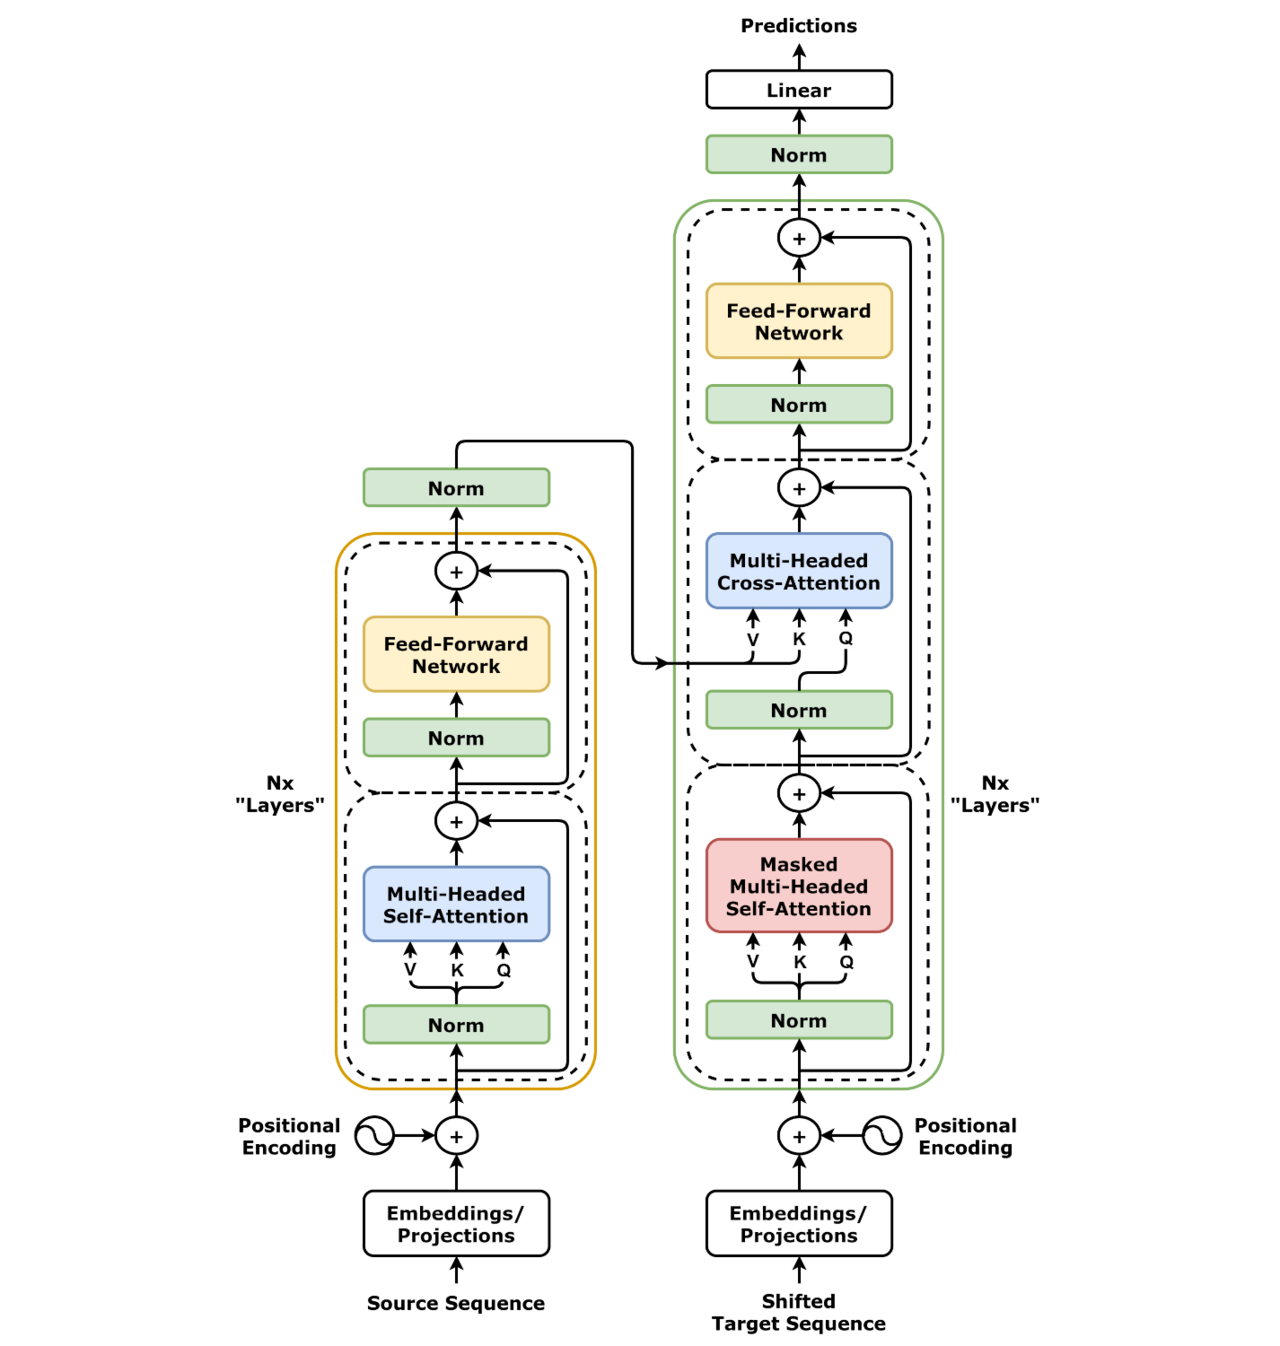
\includegraphics[width=0.65\textwidth]{images/transformer_architecture.png}
  \caption{Transformer Architecture}
  {\emph{Source: Vaswani et al., Attention Is All You Need \cite{vaswani2023attentionneed}}}
  \label{fig:transformer_architecture}
\end{figure}

\subsection{Attention Mechanism}
\label{sub:attention_mechanism}

The attention mechanism is a fundamental component of the transformer architecture
(Figure \ref{fig:transformer_architecture}), enabling the model to focus on
specific parts of the input sequence when generating the output. The attention mechanism
computes a weighted sum of the input tokens, where the weights are learned
during training based on the relevance of each token to the current context.

The self-attention mechanism works in this way:
\begin{enumerate}
  \item create 3 vectors from embeddings ($Q$uery, $K$ey, $V$alue) multiplying
    by 3 matrices learned during the training process;

  \item calculate a score that determines how much focus goes to different parts
    of the input sentence as it encodes a word;

  \item divide the score for more stable gradients and apply softmax;

  \item multiply each value vector by the softmax score to keep the value of the
    word it focuses on, and sink other irrelevant words;

  \item sum the weighted value vectors: this produces the output of the self-attention
    layer at this position.
\end{enumerate}

The self-attention operation computes the relevance of each token in the input
with respect to the query token using the scaled dot-product attention:

\begin{displaymath}
  \mbox{Attention}(Q, K, V) = \mbox{softmax}\left(\frac{QK^{T}}{\sqrt{d_{k}}}\right
  ) V
\end{displaymath}

where $d_{k}$ is the dimensionality of the key vectors, ensuring that the dot
products do not grow too large as input size increases. The softmax function normalizes
the scores into attention weights, which determine how much influence each token
should have on the final representation.

Multi-head attention extends this mechanism by computing multiple sets of
$Q,K,V$ matrices in parallel, allowing the model to capture different aspects of
contextual relationships:

\begin{displaymath}
  \mbox{MultiHead}(Q, K, V) = \mbox{Concat}(\mbox{head}_{1}, \dots, \mbox{head}_{h}
  ) W^{O}
\end{displaymath}

where each attention head independently applies scaled dot-product attention, and
the outputs are concatenated and linearly projected using $W^{O}$ ($W$eight matrix).
This improves the model's ability to encode complex dependencies and contextual meaning.

The attention mechanism allows the model to focus on different parts of the input
sequence based on the current context, enabling it to capture long-range
dependencies and improve performance on tasks like text generation.

\subsection{LLMs' Uncertainty}
\label{sub:llms_uncertainty}

Despite their impressive capabilities, LLMs are inherently probabilistic and can
generate responses that are syntactically correct yet factually inaccurate. Understanding
and quantifying this uncertainty is crucial for evaluating the reliability of generated
text, especially in high-stakes applications such as medical diagnosis, legal advice,
or automated decision-making.

For example, if an LLM generates an answer to a yes/no question with probabilities:
\begin{displaymath}
  P(\mbox{Yes})=0.51,P(\mbox{No})=0.49
\end{displaymath}

then the model is nearly uncertain, and this information should be communicated
rather than presenting ``Yes" as a definitive response.

A key consequence of uncertainty is the phenomenon of \emph{hallucination}, where
the model generates confident but factually incorrect or fabricated information \cite{Ji_2023}.
Hallucinations arise when:
\begin{itemize}
  \item the model lacks knowledge about a specific query but still generates an answer;

  \item the training data contains conflicting or misleading patterns;

  \item the model overgeneralizes from limited training examples.
\end{itemize}

Mitigating hallucinations involves uncertainty-aware generation techniques, the most
common one is \emph{Retrieval-Augmented Generation} (RAG)
\cite{lewis2021retrievalaugmentedgenerationknowledgeintensivenlp}, which enhances
the prompt with additional context from a knowledge base to improve the model's factual
accuracy.

The literature studied different approaches to quantify uncertainty in LLMs, and
this thesis will use one of the most common methods to quantify the probability
of correctness in the generated choice by the agent.

\subsubsection{Expressing Uncertainty}
A study titled `Can LLMs Express Their Uncertainty? An Empirical Evaluation of
Confidence Elicitation in LLMs' \cite{xiong2024llmsexpressuncertaintyempirical} investigates
methods for eliciting confidence from LLMs without accessing their internal parameters
or fine-tuning. The researchers propose a framework comprising three components:
\begin{itemize}
  \item Prompting Strategies: Techniques to elicit verbalized confidence from
    the model;

  \item Sampling Methods: Generating multiple responses to assess variability;

  \item Aggregation Techniques: Computing consistency across responses to
    determine confidence levels.
\end{itemize}

The study evaluates these methods on tasks such as confidence calibration and
failure prediction across various datasets and LLMs, including GPT-4 and LLaMA 2
Chat.

Key findings indicate that LLMs often exhibit overconfidence when verbalizing their
certainty, possibly mirroring human confidence expression patterns. Additionally,
as model capabilities increase, both calibration and failure prediction performance
improve, though they remain suboptimal. They show that implementing strategies like
human-inspired prompts and assessing consistency among multiple responses can mitigate
overconfidence. Notably, while methods requiring internal model access perform better,
the performance gap is narrow.

\subsubsection{Stable Explanations as Confidence Measures}
In the pursuit of reliable uncertainty quantification in Large Language Models, the
paper `Cycles of Thought: Measuring LLM Confidence through Stable Explanations '
\cite{becker2024cyclesthoughtmeasuringllm} introduced a novel framework that assesses
model confidence through the stability of generated explanations.

Their approach posits that the consistency of explanations accompanying an answer
can serve as a proxy for the model's certainty. Instead of assigning a single
probability to an answer, the method generates multiple explanations for the same
question and treats each explanation-answer pair as a distinct classifier. A
posterior distribution is then computed over these classifiers, allowing for a principled
estimation of confidence based on explanation stability. If the model's
explanations remain stable across different reasoning paths, it suggests high confidence
in the answer. Conversely, significant variation in explanations signals uncertainty.
Empirical evaluations across multiple datasets demonstrated that this framework
enhances confidence calibration and failure prediction, outperforming traditional
baselines.

However, there are some potential drawbacks. The method requires generating multiple
explanations, which increases computational cost and latency. Additionally, it
can be sensitive to prompt variations, and may misinterpret repetitive patterns as
high confidence.

\subsubsection{Tokens' log-probability}
\label{ssub:tokens_log_probability} The paper `Robots That Ask For Help: Uncertainty
Alignment for Large Language Model Planners'
\cite{ren2023robotsaskhelpuncertainty} introduces the KnowNo framework, which is
the one we took inspiration from, to quantify the uncertainty of the agent in
this thesis.

The KnowNo framework leverages Conformal Prediction (CP)\footnote{\url{https://en.wikipedia.org/wiki/Conformal_prediction}},
a statistical method that provides formal guarantees on the reliability of
predictions to assess uncertainty.

In the paper, they ask the LLM to generate a set of four actions for a given prompt
(since the \texttt{logit\_bias} parameter in the OpenAI API was limited to five tokens
at that time, more on this in Section \ref{sub:closed_source_models_openai}),
and then they append a ``no-op" action to the set. This will not be the case of
this thesis, since the actions will always be the same, but we will use the same
math behind the uncertainty calculation.

Then, they ask the model for the action to select, adding the bias to the tokens
representing each action. Here they use the log-probabilities of the tokens (referring
to the actions) to compute the uncertainty.

KnowNo computes uncertainty evaluating the ``validity" of each option: CP calculates
a confidence interval based on previous data, and from this, a set of valid actions
is generated (based on their scaled log-probability). This set can include one
or more actions, and the size of this set is indicative of the level of uncertainty:
\begin{itemize}
  \item \textbf{Singleton}: If CP narrows down the options to just one action,
    this indicates low uncertainty, and the robot can proceed confidently with the
    task. The model is highly certain that this action is the most appropriate
    next step.

  \item \textbf{Multiple Options}: When CP leaves multiple possible actions in the
    valid set, this may indicate high uncertainty. In such cases, KnowNo
    triggers the robot to request human assistance. This allows the robot to seek
    clarification when it is unsure, thereby avoiding errors that might arise
    from acting on uncertain predictions.
\end{itemize}

\begin{figure}[h!]
  \centering
  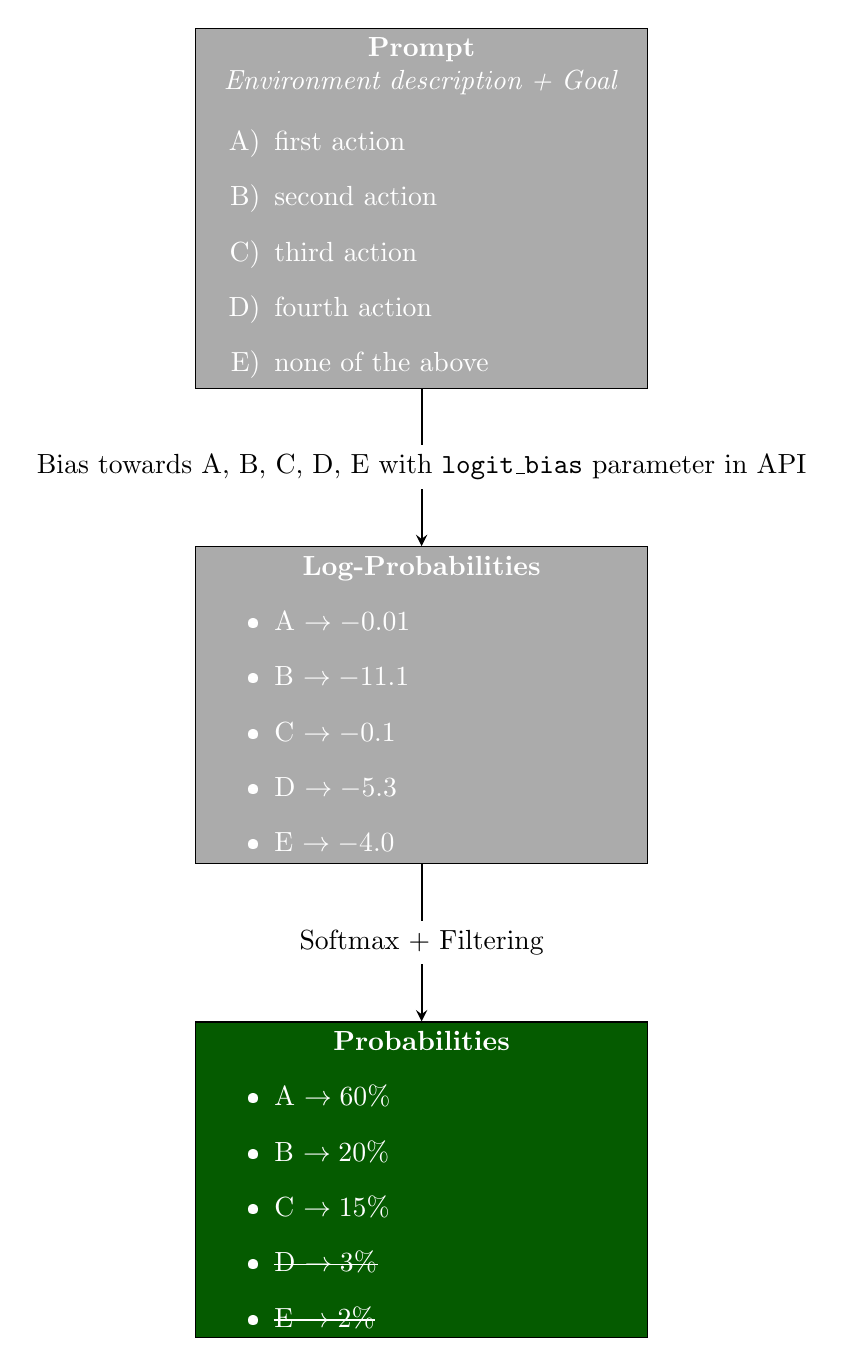
\begin{tikzpicture}
    % Define styles
    \tikzstyle{block}
    = [rectangle, draw, text width=5.5cm, align=center, minimum height=2cm]
    \tikzstyle{arrow}
    = [thick, ->, >=stealth]

    % Nodes
    \node[
      block,
      text centered,
      fill={rgb,255:red,171; green,171; blue,171},
      text=white
    ]
      (prompt)
      { \textbf{Prompt} \\ \emph{Environment description + Goal} \\\begin{itemize}\item[A)] first action

      \item[B)] second action

      \item[C)] third action

      \item[D)] fourth action

      \item[E)] none of the above\end{itemize}};

    \node[
      block,
      below=of prompt,
      text centered,
      yshift=-1cm,
      fill={rgb,255:red,171; green,171; blue,171},
      text=white
    ]
      (logprob)
      { \textbf{Log-Probabilities}\begin{itemize}\item A $\to -0.01$

      \item B $\to -11.1$

      \item C $\to -0.1$

      \item D $\to -5.3$

      \item E $\to -4.0$\end{itemize}};

    \node[
      block,
      below=of logprob,
      text centered,
      yshift=-1cm,
      fill={rgb,255:red,5; green,91; blue,0},
      text=white
    ]
      (prob)
      { \textbf{Probabilities}\begin {itemize} \item A $\to 60\%$ \item B $\to 20\%$ \item C $\to 15\%$ \item \sout {D $\to 3\%$} \item \sout {E $\to 2\%$} \end{itemize}};

    % Arrows
    \draw[arrow]
      (prompt.south) -- (logprob.north)
      node[midway, fill=white, text centered]
        {Bias towards A, B, C, D, E with \texttt{logit\_bias} parameter in API};
    \draw[arrow]
      (logprob.south) -- (prob.north)
      node[midway, fill=white, text centered] {Softmax + Filtering};
  \end{tikzpicture}
  \caption{KnowNo Uncertainty Computation}
  \label{fig:knowno_flow}
\end{figure}

A simplified version of the KnowNo flow can be seen in Figure
\ref{fig:knowno_flow}. Technically speaking, the computation of the uncertainty
can be summarize in 5 steps:
\begin{enumerate}
  \item give each action a single-token label (eg. \texttt{A)}, \texttt{B)}, \texttt{C)},
    \texttt{D)}, \texttt{E)});

  \item use the \texttt{logit\_bias} parameter in the API to force the model to
    only answer using these labels;

  \item get the log-probabilities of the tokens and scale them: this results in
    a ``confidence" value for each token;

  \item filter the resulting set of option with a threshold computed with CP;

  \item either the result will be a singleton (no uncertainty) or a set of options.
\end{enumerate}

They also say that the framework has the advantage of being model-agnostic, as it
can be applied to LLMs out-of-the-box without requiring any fine-tuning, thanks
to the ``caution" that is given if the resulting filtered set of options is not a
singleton.

\section{Agents}
\label{sec:agents}

% \begin{figure}[h!]
%   \label{fig:agent_scheme}
%   \centering
%   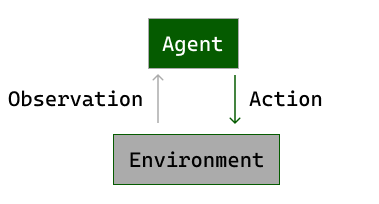
\includegraphics[width=.3333\textwidth]{images/Agent_Scheme.png}
%   \caption{Agent Scheme}
%   { Source: redesign of a scheme in \cite{wooldridge2002multiagent}}
% \end{figure}

As widely explained in the book `An Introduction to Multiagent Systems' \cite{wooldridge2002multiagent},
we can summarize the definition of an agent as an autonomous entity that
perceives its environment through sensors and acts upon it through effectors, making
decisions based on its perceptions and objectives in order to achieve specific goals.

This definition highlights several key aspects of agents:
\begin{itemize}
  \item Autonomy: Agents operate without direct human intervention, controlling their
    own actions.

  \item Perception and Action: They interact with the environment via sensors (perception)
    and actuators (action execution).

  \item Decision-making: Agents select actions based on their internal model, goals,
    and the state of the environment.

  \item Non-determinism and Adaptability: Since environments are generally non-deterministic,
    agents must be prepared for uncertainty and potential failures in action execution.

  \item Preconditions and Constraints: Actions are subject to certain conditions
    that must be met for successful execution.
\end{itemize}

Thus, an agent's fundamental challenge is deciding which actions to perform in
order to best satisfy its objectives, given the constraints and uncertainties of
its environment.

\vspace{1cm} % Add margin on top
\begin{figure}[h!]
  \centering
  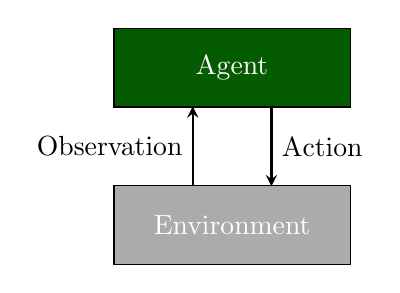
\begin{tikzpicture}[
    node distance=2cm, % Distance between nodes
  ]
    \node[
      rectangle,
      minimum width=3cm,
      minimum height=1cm,
      text centered,
      draw=black,
      fill={rgb,255:red,5; green,91; blue,0},
      text=white
    ] (agent) {Agent};
    \node[
      rectangle,
      minimum width=3cm,
      minimum height=1cm,
      text centered,
      draw=black,
      below of=agent,
      fill={rgb,255:red,171; green,171; blue,171},
      text=white
    ] (env) {Environment};

    % First arrow (Action) slightly shifted right
    \draw[thick, ->, >=stealth]
      (agent.south)
      ++(0.5,0) -- ++(0,-1)
      node[midway, right] {Action};

    % Second arrow (Observation) slightly shifted left
    \draw[thick, ->, >=stealth]
      (env.north)
      ++(-0.5,0) -- ++(0,1)
      node[midway, left] {Observation};
  \end{tikzpicture}
  \caption{Agent Design Scheme}
  {\emph{Source: redesign of a scheme in \cite{wooldridge2002multiagent}}} \label{fig:agent_scheme}
\end{figure}
\vspace{1cm} % Add margin on bottom

As shown in Figure \ref{fig:agent_scheme}, an agent is some entity that perceives
the environment and reacts to it. The setting can be anything from a simple
thermostat to a complex system like a self-driving car. The idea is that the agent
is able to react to a change in the environment and take actions to achieve its goals.

We will analyze in detail the prompts and the choices in Section \ref{sec:prompts},
but to give an some anticipation to align our agent with the definition above, we
can map some of its concept to what this thesis will analyze:
\begin{itemize}
  \item Autonomy: the agent will choose its action based on the prompt built
    using the environment information only;

  \item Perception and Action: what the server sends about the current state of
    the environment can be seen as the perception of the agent, while the action
    it can take will be given in the prompt in a specific way.

  \item Decision-making: the decision-making process will be the generation of
    the text by the LLM, weighted by the uncertainty.

  \item Non-determinism and Adaptability: to emulate the non-determinism of the
    environment, the state received by the server will be used ``raw" in the
    prompt, without any hard processing or parsing.

  \item Preconditions and Constraints: being in a ``limited" map with a fixed number
    of walkable cells, is itself a constraint the agent must consider.
\end{itemize}

\subsection{BDI Architecture}
\label{sub:bdi_architecture}

The Belief-Desire-Intention (BDI) architecture is a widely adopted framework in
artificial intelligence for modeling rational agents. It was formally developed by
Rao and Georgeff in 1995 \cite{bdi-icmas95} and has been implemented in several architectures,
including PRS (1987), dMARS (1998), JAM (1999), Jack (2001), and JADEX (2005). BDI
provides a structured approach to practical reasoning, allowing agents to
function effectively in dynamic and unpredictable environments.

\subsubsection{Core Components of BDI}
BDI agents operate based on three key components:
\begin{itemize}
  \item Belief: Represents the agent's knowledge about the world, including past
    events and observations;

  \item Desire (Goals): Defines the agent's objectives or preferred end states;

  \item Intention: Represents the commitments of an agent toward achieving
    specific goals through selected plans.
\end{itemize}

BDI has been extensively used in fields like robotics, automated planning, and
multi-agent systems.

\section{State of the Art}
\label{sec:state_of_the_art}

A logistic problem is a fundamental challenge in the field of Artificial Intelligence
(AI), since depending on the complexity of the specific problem, it can contain tasks
such as route optimization, supply chain management, and delivery scheduling.
These problems arise in various domains, including transportation, e-commerce, and
manufacturing, where efficient resource allocation and decision-making are
critical. Given the complexity of modern logistics, AI has emerged as a powerful
tool for finding optimal or near-optimal solutions.

Traditional research techniques, such as linear programming and heuristics, have
been widely employed. However, with the increasing availability of data and
computational power, machine learning (ML) and deep learning methods have become
more prevalent. These methods can predict demand, optimize routes dynamically,
and enhance decision-making under uncertainty based on the data. Additionally,
reinforcement learning (RL) has gained attention for its ability to learn
optimal strategies through trial and error, particularly in dynamic and unpredictable
environments.

In the recent years with the explosion of Large Language Models (LLMs), many
researchers started to apply them to different fields, including planning and logistics.

% \begin{quotation}
%   This is a longer blockquote that may span multiple paragraphs. It is indented
%   on both sides.
% \end{quotation}

\subsection{PDDL Based Solutions}
\label{sub:pddl_based_solutions}
\begin{blockquote}
  \textbf{Planning Domain Definition Language} (PDDL) is a human-readable format
  for problems in automated planning that gives a description of the possible
  states of the world, a description of the set of possible actions, a specific
  initial state of the world, and a specific set of desired goals.

  \emph{Source: Wikipedia\footnotemark}
\end{blockquote}
\footnotetext{\url{https://en.wikipedia.org/wiki/Planning_Domain_Definition_Language}}

The fundamental distinction between a PDDL-based solution and any Machine Learning/Deep
Learning approach lies in the very nature of how problems are defined and solved.

In a PDDL-based system, the problem must be explicitly encoded using a formal, structured
language that describes the initial state, the goal state, and the set of available
actions. This formal encoding serves as a blueprint for the planner, which then performs
the computationally intensive task of exploring a vast search space. The planner
systematically generates and evaluates possible action sequences, using algorithms
to determine an optimal path from the initial state to the goal state. This
process is highly deterministic, with each action being considered in the context
of its direct impact on reaching the goal.

While effective in structured, static environments with well-defined parameters,
this approach is inherently time-consuming and computationally demanding. The
planner must traverse a potentially enormous state space, guided by heuristics to
prune less relevant possibilities, but still constrained by the rigid formalism
of PDDL. Because of this, it can struggle with real-time decision-making, particularly
in situations where the environment is dynamic, uncertain, or rapidly changing.

\vspace{10mm}
\begin{codewindow}
  [PDDL Code] \lstset{style=pddlstyle, language=PDDL, caption={Domain file example for a bit toggle problem},
  label={lst:domain_file_toggle_bits}} \begin{lstlisting}
(define (domain bit-toggle)
  (:requirements :strips :negative-preconditions)
  (:predicates
    (bit ?b)                       ; predicate meaning
                                   ; bit ?b is set (true)
  )

  (:action setbit
    :parameters (?b)
    :precondition (not (bit ?b))   ; can only set a bit if
                                   ; it is not already set
    :effect (bit ?b)               ; setting the bit to true
  )

  (:action unsetbit
    :parameters (?b)
    :precondition (bit ?b)         ; can only unset a bit if
                                   ; it is currently set
    :effect (not (bit ?b))         ; setting the bit to false
  )
)

\end{lstlisting}
\end{codewindow}
\vspace{10mm}

\vspace{10mm}
\begin{codewindow}
  [PDDL Code] \lstset{style=pddlstyle, language=PDDL, caption={Problem file example for a bit toggle problem},
  label={lst:problem_file_toggle_bits}} \begin{lstlisting}
(define (problem bit-toggle-full-problem)
  (:domain bit-toggle-full)
  (:objects
     b1 b2 b3
  )
  (:init)                          ; Initially all bits are unset (false)

  (:goal                           ; It can be any combination of T/F
     (and (bit b1) (bit b2) (not(bit b3)))
  )
)
\end{lstlisting}
\end{codewindow}
\vspace{10mm}

With the increasing number of variables (actions or predicates), the number of
arcs and nodes grows exponentially. A little example that makes this problem easy
to visualize is the Domain where we can have N possible bits, that can be turned
to \texttt{true} or \texttt{false} (Domain file in Listing \ref{lst:domain_file_toggle_bits})
and the Problem where everything start at \texttt{false} and we want a specific final
combination (Problem file in Listing \ref{lst:problem_file_toggle_bits}).

\begin{figure}[h!]
  \noindent
  \begin{minipage}{0.33\textwidth}
    \centering
    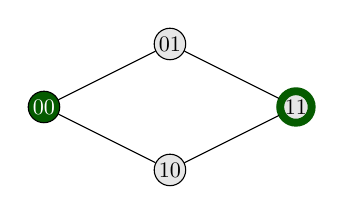
\begin{tikzpicture}[
      scale=0.8,
      transform shape,
      nodes={draw, circle, minimum size=5mm, inner sep=0pt}
    ]
      % First plot
      \node (00) at (0,0) [fill=primary, text=white] {00};
      \node (01) at (2,1) [fill=code-bg] {01};
      \node (10) at (2,-1) [fill=code-bg] {10};
      \node (11)
        at
        (4,0)
        [fill=code-bg, thick, draw=primary, line width=1mm]
        {11};
      \draw (00) -- (01);
      \draw (00) -- (10);
      \draw (01) -- (11);
      \draw (10) -- (11);
    \end{tikzpicture}

    \vspace{1cm} % Space between first and second plot

    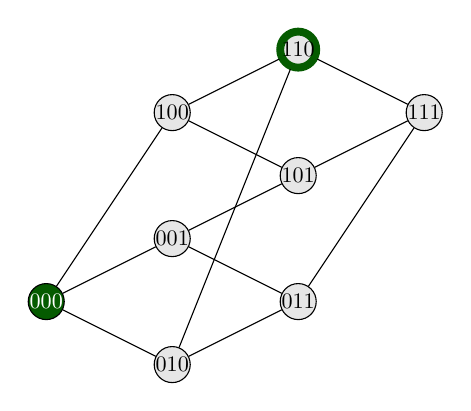
\begin{tikzpicture}[
      scale=0.8,
      transform shape,
      nodes={draw, circle, minimum size=5mm, inner sep=0pt}
    ]
      % Second plot
      \node (000) at (0,0) [fill=primary, text=white] {000};
      \node (001) at (2,1) [fill=code-bg] {001};
      \node (010) at (2,-1) [fill=code-bg] {010};
      \node (011) at (4,0) [fill=code-bg] {011};
      \node (100) at (2,3) [fill=code-bg] {100};
      \node (101) at (4,2) [fill=code-bg] {101};
      \node (110)
        at
        (4,4)
        [fill=code-bg, thick, draw=primary, line width=1mm]
        {110};
      \node (111) at (6,3) [fill=code-bg] {111};
      \draw (000) -- (001);
      \draw (000) -- (010);
      \draw (000) -- (100);
      \draw (001) -- (011);
      \draw (001) -- (101);
      \draw (010) -- (011);
      \draw (010) -- (110);
      \draw (100) -- (101);
      \draw (100) -- (110);
      \draw (011) -- (111);
      \draw (101) -- (111);
      \draw (110) -- (111);
    \end{tikzpicture}
  \end{minipage}
  \hfill
  \begin{minipage}{0.66\textwidth}
    \centering
    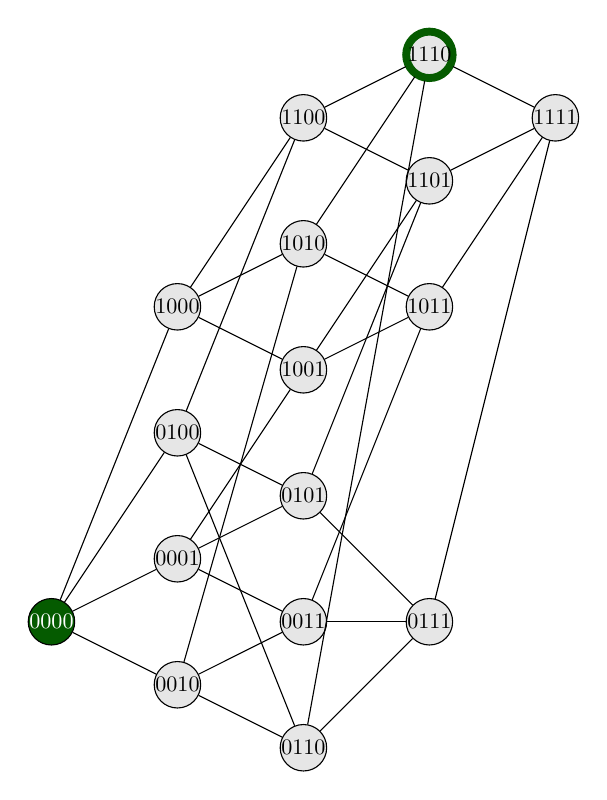
\begin{tikzpicture}[
      scale=0.8,
      transform shape,
      nodes={draw, circle, minimum size=5mm, inner sep=0pt}
    ]
      % Third plot
      \node (0000) at (0,0) [fill=primary, text=white] {0000};
      \node (0001) at (2,1) [fill=code-bg] {0001};
      \node (0010) at (2,-1) [fill=code-bg] {0010};
      \node (0011) at (4,0) [fill=code-bg] {0011};
      \node (0100) at (2,3) [fill=code-bg] {0100};
      \node (0101) at (4,2) [fill=code-bg] {0101};
      \node (0110) at (4,-2) [fill=code-bg] {0110};
      \node (0111) at (6,0) [fill=code-bg] {0111};
      \node (1000) at (2,5) [fill=code-bg] {1000};
      \node (1001) at (4,4) [fill=code-bg] {1001};
      \node (1010) at (4,6) [fill=code-bg] {1010};
      \node (1011) at (6,5) [fill=code-bg] {1011};
      \node (1100) at (4,8) [fill=code-bg] {1100};
      \node (1101) at (6,7) [fill=code-bg] {1101};
      \node (1110)
        at
        (6,9)
        [fill=code-bg, thick, draw=primary, line width=1mm]
        {1110};
      \node (1111) at (8,8) [fill=code-bg] {1111};
      \draw (0000) -- (0001);
      \draw (0000) -- (0010);
      \draw (0000) -- (0100);
      \draw (0000) -- (1000);
      \draw (0001) -- (0011);
      \draw (0001) -- (0101);
      \draw (0001) -- (1001);
      \draw (0010) -- (0011);
      \draw (0010) -- (0110);
      \draw (0010) -- (1010);
      \draw (0011) -- (0111);
      \draw (0011) -- (1011);
      \draw (0100) -- (0101);
      \draw (0100) -- (0110);
      \draw (0100) -- (1100);
      \draw (0101) -- (0111);
      \draw (0101) -- (1101);
      \draw (0110) -- (0111);
      \draw (0110) -- (1110);
      \draw (0111) -- (1111);
      \draw (1000) -- (1001);
      \draw (1000) -- (1010);
      \draw (1000) -- (1100);
      \draw (1001) -- (1011);
      \draw (1001) -- (1101);
      \draw (1010) -- (1011);
      \draw (1010) -- (1110);
      \draw (1011) -- (1111);
      \draw (1100) -- (1101);
      \draw (1100) -- (1110);
      \draw (1101) -- (1111);
      \draw (1110) -- (1111);
    \end{tikzpicture}
  \end{minipage}
  \caption{Graphs for bit-toggle problem with 2, 3, and 4 bits}
  \label{fig:bit_toggle_graphs}
\end{figure}

\begin{figure}[h!]
  \centering
  \subfloat[
  \centering
  label 1]{{ 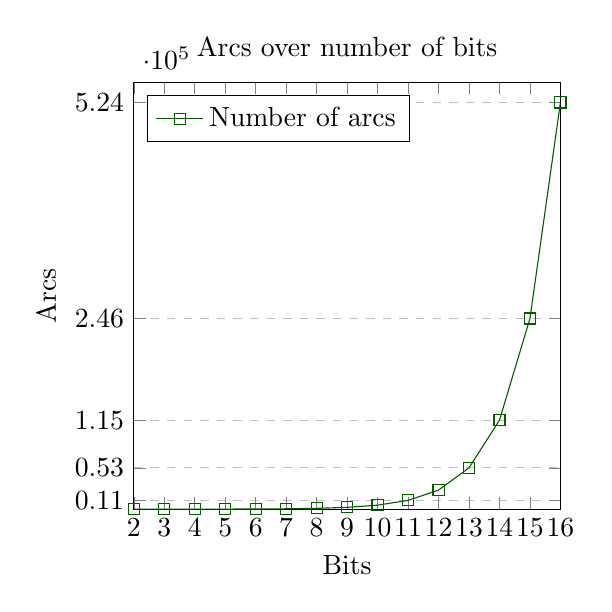
\begin{tikzpicture}\begin{axis}[ title={Arcs over number of bits}, xlabel={Bits}, ylabel={Arcs}, width=7cm, height=7cm, xmin=2, xmax=16, ymin=4, ymax=550000, xtick={2,3,4,5,6,7,8,9,10,11,12,13,14,15,16}, ytick={11264,53248,114688,245760, 524288}, legend pos=north west, ymajorgrids=true, grid style=dashed, ]\addplot[ color=primary, mark=square, ] coordinates { (2,4)(3,12)(4,32)(5,80)(6,192)(7,448)(8,1024)(9,2304)(10,5120)(11,11264)(12,24576)(13,53248)(14,114688)(15,245760)(16,524288) }; \legend{Number of arcs}\end{axis}\end{tikzpicture} }}
  \qquad \subfloat[
  \centering
  label 1]{{ 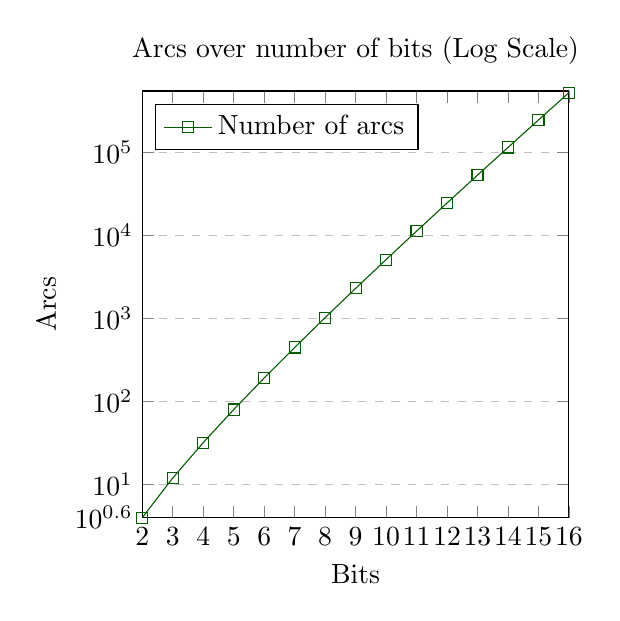
\begin{tikzpicture}\begin{semilogyaxis}[ title={Arcs over number of bits (Log Scale)}, xlabel={Bits}, ylabel={Arcs}, width=7cm, height=7cm, xmin=2, xmax=16, ymin=4, ymax=550000, xtick={2,3,4,5,6,7,8,9,10,11,12,13,14,15,16}, ytick={4,10,100,1000,10000,100000}, legend pos=north west, ymajorgrids=true, grid style=dashed, ] \addplot[ color=primary, mark=square, ] coordinates { (2,4)(3,12)(4,32)(5,80)(6,192)(7,448)(8,1024)(9,2304)(10,5120)(11,11264)(12,24576)(13,53248)(14,114688)(15,245760)(16,524288) }; \legend{Number of arcs}\end{semilogyaxis}\end{tikzpicture} }}
  \caption{Arcs per Bit}
  \label{fig:arcs_per_bit}
\end{figure}

As we can see in the plot Figure \ref{fig:arcs_per_bit}, the number of arcs (example
of graphs for 2, 3 and 4 bits in Figure \ref{fig:bit_toggle_graphs}) grows exponentially
with the number of bits, as well as the number of states obviously. This shows how
even a simple problem with a simple solution can become time-intensive and not suitable
for real-time applications.

\vspace{10mm}
\begin{codewindow}
  [PDDL Code] \lstset{style=pddlstyle, language=PDDL, caption={Plan for the bit toggle problem (\texttt{110}), solved by LAMA-first planner},
  label={lst:plan_toggle_bits}} \begin{lstlisting}
          ; Found Plan (output)
(setbit b2)
(setbit b1)
\end{lstlisting}
\end{codewindow}
\vspace{10mm}

However, a PDDL approach is more explainable, since all the information is
provided by the user and the output result is a sequence of actions (example at Listing
\ref{lst:plan_toggle_bits}). This makes it easier to understand and debug the solution,
as each step is explicitly defined. Of course, there might be different paths to
reach the goal, and the planner might choose one based on heuristics or optimization
criteria. This transparency in the decision-making process is one of the key
advantages of using PDDL for planning problems.

\paragraph{Literature}
An example of a problem related to the one presented in this thesis, solved
using PDDL, can be found in the paper `An AI Planning Approach to Emergency
Material Scheduling Using Numerical PDDL' by Yang et al. \cite{Yang2022}.

In their work, they utilize PDDL 2.1 that allows to model the scheduling problem,
incorporating factors such energy consumption constraints. Their approach employs
the Metric-FF planner to generate optimized scheduling plans that minimize total
scheduling time and transportation energy usage. However, while this demonstrates
the applicability of AI planning to emergency logistics, their model simplifies
the real-world scenario by assuming predefined transport routes, limited vehicle
types, and abstract representations of congestion effects. This highlights a broader
limitation of PDDL in capturing the full complexity of dynamic and uncertain environments
often encountered in emergency response situations.

\subsection{Reinforcement Learning Solutions}
\begin{blockquote}
  \textbf{Reinforcement Learning} is a branch of machine learning focused on
  making decisions to maximize cumulative rewards in a given situation. Unlike supervised
  learning, which relies on a training dataset with predefined answers, RL involves
  learning through experience. In RL, an agent learns to achieve a goal in an uncertain,
  potentially complex environment by performing actions and receiving feedback
  through rewards or penalties.

  \emph{Source: GeegksforGeeks \footnotemark}
\end{blockquote}
\footnotetext{\url{https://www.geeksforgeeks.org/what-is-reinforcement-learning/}}

Reinforcement Learning is a learning setting, where the learner is an Agent that
can perform a set of actions depending on its state in a set of states and the environment.

It works by defining:
\begin{itemize}
  \item \textbf{Environment}: the world in which the agent operates

  \item \textbf{Agent}: the decision-maker that interacts with the environment

  \item \textbf{Actions}: the possible moves the agent can make

  \item \textbf{Rewards}: the feedback the agent receives for its actions

  \item \textbf{Policy}: the strategy the agent uses to select Actions
\end{itemize}

In performing action \texttt{a} in state \texttt{s}, the learner receive an
immediate reward \texttt{r(s,a)}. In some states, some actions could be not possible
or valid.

The task is to learn a policy (a full specification of what action to take at
each state) allowing the agent to choose for each state the action maximizing the
overall reward, including future moves.

To deal with this delayed reward problem, the agent has to trade-off exploitation
and exploration:
\begin{itemize}
  \item \textbf{Exploitation}: the agent chooses the action that it knows will give
    some reward

  \item \textbf{Exploration}: the agent tries alternative actions that could end
    in bigger rewards
\end{itemize}

When considering a logistics problem, reinforcement learning naturally comes to
mind. This is because defining a reward function is relatively straightforward:
it could be measured in terms of packages delivered per minute, per step, or a
similar metric. Additionally, the entire process can be simulated in a virtual
environment, allowing multiple parallel simulations to accelerate the agent's learning
process. As illustrated in Figure \ref{fig:rl_scheme}, the structure of the Reinforcement
Learning framework closely resembles the agent-based model depicted in Figure \ref{fig:agent_scheme}.
In both cases, the agent interacts with its environment, receives feedback in
the form of rewards, and continuously refines its policy to optimize future performance.

\begin{figure}[h!]
  \centering
  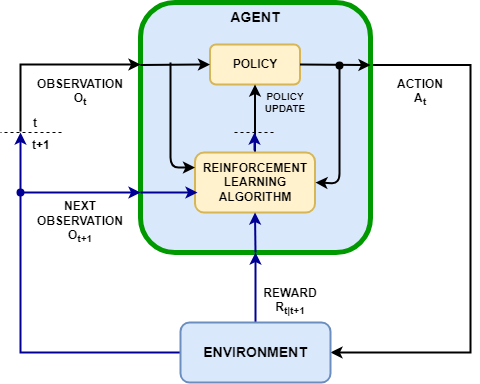
\includegraphics[width=.6\textwidth]{images/rl_scheme.png}
  \caption{RL Agent Scheme}
  {\emph{Source: Mathworks}\footnotemark} \label{fig:rl_scheme}
\end{figure}
\footnotetext{\url{https://it.mathworks.com/help/reinforcement-learning/ug/create-agents-for-reinforcement-learning.html}}

However, RL has its own set of challenges. The most common one is the
convergence to a local minimum in the reward function. This means that the agent
might become stuck in suboptimal strategy that is not the best one. Moreover, RL
is not explainable, meaning that we can't understand why the agent took a
specific action in a specific situation.

Another issue with RL is the cost of training. Since the agent learns through trial
and error, it needs to perform a large number of actions to explore the
environment and learn the best strategy. This can be computationally expensive and
time-consuming, especially for complex problems with many variables and states. Moreover,
once the agent is trained, its adaptability to new environments or situations is
limited, as it is optimized for a specific reward function and environment
configuration.

\paragraph{Literature}
An example of a problem similar to the one presented in this thesis, solved
using Reinforcement Learning, can be found in the paper `DeliverAI: a distributed
path-sharing network based solution for the last mile food delivery problem' by
Ashman et al. \cite{mehra2024deliveraireinforcementlearningbased}.

They aimed at solving the last-mile delivery problem by developing a distributed
path-sharing network based on Reinforcement Learning. Their approach uses a
multi-agent system to optimize delivery routes and schedules, considering factors
such as traffic congestion, delivery time windows, and vehicle capacity.

However, their model simplifies the real-world scenario by assuming fixed
delivery locations and known traffic patterns, which may not accurately reflect the
dynamic and uncertain nature of real-world logistics environments. Moreover, their
approach requires extensive training and tuning to achieve optimal performance.

\subsection{Planning with LLM}
\label{sub:planning_in_llm}

LLMs are trained on vast amounts of textual data and have demonstrated
remarkable performance across a wide range of language tasks, from translation and
summarization to reasoning and problem-solving. This success has naturally led
researchers to explore whether these models can be repurposed for more complex, multi-step
decision-making problems that require planning.

The key idea is that the same abilities that allow LLMs to understand and generate
language can be harnessed to decompose a planning task into intermediate steps,
reason about the consequences of actions, and even generate entire action sequences
with minimal or no task-specific training.

\subsubsection{Chain-of-Thought Reasoning}

One of the most influential ideas for using LLMs in planning is Chain-Of-Thought
(CoT) prompting. Instead of asking the model to jump directly from a problem statement
to a final answer, CoT prompting encourages the model to ``think aloud" by generating
intermediate reasoning steps. This decomposition can help in planning problems
where the solution involves multiple, logically connected steps.

This was first discovered by Wei et al.
\cite{wei2023chainofthoughtpromptingelicitsreasoning}, who demonstrated that prompting
the LLM to 'answer step by step' led to improved performance on mathematical problems
compared to requesting only the final answer. They also showed that this step-by-step
approach could be applied to other fields, ultimately giving rise to Chain-of-Thought
reasoning models.

\paragraph{``Reasoning" Models}
Reasoning-focused LLMs are trained to generate multiple Chain-of-Thought steps, exploring
different solution paths before selecting the most optimal one, often using
Reinforcement Learning
\cite{deepseekai2025deepseekr1incentivizingreasoningcapability} techniques such
as RLHF (Reinforcement Learning from Human Feedback) or self-consistency methods
during the training.

This approach enhances both accuracy and explainability, as the model articulates
its reasoning process while still operating as a generative AI system. Expanding
on this concept, reasoning models can integrate external tools, memory, and API calls,
forming what is commonly referred to as an LLM Agent, capable of autonomous decision-making
and real-world interaction.

Most recent and famous reasoning models released to the public have been developed
by many companies, both big and small, such as:
\begin{itemize}
  \item \textbf{OpenAI}: o1\footnote{\url{https://openai.com/o1/}}, o1-mini\footnote{\url{https://openai.com/index/openai-o1-mini-advancing-cost-efficient-reasoning/}}
    and o3-mini\footnote{\url{https://openai.com/index/openai-o3-mini/}} are reasoning
    models designed to enhance logical problem-solving capabilities. o1 is
    specialized in complex problems across various domains, offering robust reasoning
    skills. Building upon this foundation, o3-mini provides a more cost-effective
    and faster alternative;

  \item \textbf{DeepSeek}: DeepSeek-R1\footnote{\url{https://github.com/deepseek-ai/DeepSeek-R1}},
    is a notable AI model from a startup\footnote{\url{https://www.deepseek.com/}}.
    Released in early 2025, DeepSeek-R1 is recognized for its powerful reasoning
    and coding skills, achieved at a fraction of the development cost compared to
    other leading models. Its open-source nature and efficiency have made it a
    significant player in the AI landscape.
\end{itemize}

\subsubsection{Zero-Shot and Few-Shot Planning}
In zero-shot planning, LLMs generate action sequences by utilizing their
extensive pretraining on text and code, effectively inferring plausible step-by-step
solutions to given tasks. Few-shot planning further enhances this by providing
LLMs with a small set of demonstrations, enabling them to generalize patterns and
improve their action sequencing capabilities.

However, while LLMs can produce reasonable plans, their direct applicability to embodied
environments remains challenging. Huang et al. \cite{huang2022languagemodelszeroshotplanners}
highlight the limitations of naive LLM planning, noting that LLMs struggle with
real-world constraints, action feasibility, and long-horizon dependencies. Their
work demonstrates that these shortcomings can be mitigated by leveraging the world
knowledge embedded within LLMs and applying structured guidance, such as
constraints on action generation and feedback-based refinements.

Similarly, Silver et al. \cite{silver2022pddl} extend this inquiry to classical
AI planning domains by evaluating few-shot prompting of LLMs on problems
expressed in the Planning Domain Definition Language (PDDL). Their findings reveal
mixed results: while LLMs can generate syntactically correct PDDL plans in
certain domains, they often fail due to a lack of explicit access to transition models
and logical constraints inherent to planning problems. Nonetheless, their study also
introduces a hybrid approach where LLMs are used to initialize heuristic-based search
planners, demonstrating that even imperfect LLM-generated plans can improve the
efficiency of traditional AI planning methods.

These findings collectively suggest that while LLMs alone are not yet fully
capable of robust autonomous planning, their ability to extract and apply commonsense
knowledge makes them valuable tools for augmenting structured planning frameworks.
By integrating LLM-generated outputs with classical search-based methods, researchers
have shown improvements in planning efficiency and problem-solving robustness,
highlighting a promising direction for future research at the intersection of
language models and automated planning.

\paragraph{Literature}
In the paper `Exploring and Benchmarking Planning Capabilities of Large Language
Models' by Bohnet et al.
\cite{bohnet2024exploringbenchmarkingplanningcapabilities}, the authors systematically
analyze the planning capabilities of LLMs through a novel benchmarking suite that
includes both classical planning tasks (expressed in PDDL) and natural language-based
planning problems. Their work highlights the limitations of LLMs in planning, particularly
their tendency to generate suboptimal or incorrect plans despite their strong language
understanding capabilities. To address these shortcomings, they explore various methods
to improve LLM-based planning (including many-shot in-context learning, fine-tuning
with optimal plans, and the use of chain-of-thought reasoning techniques such as
Monte Carlo Tree Search (MCTS) and Tree-of-Thought (ToT)). The results indicate
that, while LLMs struggle with planning in zero-shot and few-shot settings,
their performance significantly improves when provided with structured
demonstrations and reasoning strategies. Moreover, fine-tuning on high-quality
plan data leads to near-perfect accuracy in some cases, even with relatively small
models. However, challenges remain in out-of-distribution generalization, where
models fail to generalize effectively to novel scenarios without additional
training. Their analysis also identifies key failure modes in LLM planning, such
as constraint violations, failure to reach goal states, and incorrect action
sequences, emphasizing the need for better training data curation and reasoning frameworks.

\paragraph{Literature}
In `Generalized Planning in PDDL Domains with Pretrained Large Language Models'
by Silver et al. \cite{silver2023generalizedplanningpddldomains}, the authors
investigate whether LLMs, specifically GPT-4, can serve as generalized planners,
not just solving a single planning task, but synthesizing programs that generate
plans for an entire domain. They introduce a pipeline where GPT-4 is prompted to
summarize the domain, propose a general strategy, and then implement it in Python.
Additionally, they incorporate automated debugging, where GPT-4 iteratively
refines its generated programs based on validation feedback. Their evaluation on
seven PDDL domains demonstrates that GPT-4 can often generate efficient domain-specific
planning programs that generalize well from only a few training examples. The
study also finds that automated debugging significantly improves performance, while
the effectiveness of Chain-of-Thought summarization is domain-dependent. Notably,
GPT-4 outperforms previous generalized planning approaches in some cases,
particularly when leveraging semantic cues from domain descriptions. However,
limitations remain, especially in handling domains requiring deeper structural reasoning
or non-trivial search processes.
  \chapter{Experiment Setting}
\label{cha:experiment_setting}
  \chapter{Agent Development}
\label{cha:agent_development}

In this chapter we present the iterative development of the agent. We describe the
successive phases of its evolution, from the initial prototype to the final
implementation. During this process, several challenges and unexpected issues
emerged. For each phase, we detail the encountered problems and the approaches
adopted to overcome them, explaining the reasoning behind the design choices.
The majority of the choices taken in the crafting of the various prompt will be
discussed in Chapter \ref{cha:data_collection}, while reporting here all the discarded
ones.

\section{Development information}
\label{sec:development_information}

The go-to programming language for AI development is Python. However, we chose
to use JavaScript for this project for several reasons. First, both the server
and the example agents were already implemented in JavaScript; so a JavaScript interface
to communicate with the server was already available. This allowed us to focus
only on the agent's logic, without having to worry about the server's implementation.
Second, thanks to the availability of the project of the Autonomous Software Agents
course, our initial plan was to use an existing JavaScript-based benchmark from
the course. Although we ultimately decided against using this benchmark, as
explained later, JavaScript remained our language of choice.

Additionally, since there is no more a dedicated JavaScript library for the
Azure OpenAI API, instead of manually recreating the necessary API calls we opted
for a more efficient approach by setting up a lightweight Python server to act as
a middleman. This solution, discussed in Section \ref{par:azureapi}, allowed us
to integrate Azure's services seamlessly while maintaining JavaScript for the
core development.

\section{First Approach}
\label{sec:first_approach}

In this initial phase of the development and testing process, a trial-and-error
methodology was adopted to iteratively refine the system's behavior and try to
optimize performance. Unfortunately, this led to moving away from the definition
of the problem and, in combination with the poor performance of the agent, it
was decided to start over with a new approach. Nonetheless, this first attempt
was crucial in understanding the challenges and limitations of the problem, so it
is important to describe it.

\vspace{1mm}
\begin{codewindow}
  [Text] \lstset{style=pythonstyle, caption={Scheme of a prompt used in the first approach, full in Appendix \ref{lst:apx:first_agent_prompt}},
  label={lst:first_agent_prompt}} \begin{lstlisting}
[ROLE]

[MAP]

[LEGEND]

[ACTIONS]

[PARCELS ALREADY PICKED]

[RULES]

[QUESTION]
\end{lstlisting}
\end{codewindow}
\vspace{1mm}

The approach began by parsing crucial information from the server, which served as
the foundation for understanding how the LLM would interact with it. The main
point of discuss in the parsing topic was the map, that was represented as a multi-line
string like the one in Listing \ref{lst:parced_map}. The first prompt sent to
the LLM was crafted by concatenating the map with all the other information
needed to describe the state of the environment, as shown in Listing \ref{lst:first_agent_prompt}.

\vspace{1mm}
\begin{codewindow}
  [Text] \lstset{style=pythonstyle, caption={Parsed Map Result with partial legend},
  label={lst:parced_map}} \begin{lstlisting}
    1 1 1 1 1
    1 1 P 1 1
    1 1 1 1 1
    2 A 1 1 1
    1 1 1 1 1

    LEGEND:
    1: Walkable cell
    2: Delivery point
    A: Agent
    P: Parcel
\end{lstlisting}
\end{codewindow}
\vspace{1mm}

This implementation started as a full raw approach, letting the LLM also decide the
goal to pursue. As various challenges and inefficiencies were identified during
extensive testing, we progressively implemented a total of seven ``helping"
parameters.

\subsection{Helping Parameters}
These parameters were introduced with the objective of addressing specific
issues observed during experimentation, and each of them played a significant role
in shaping the overall functionality of the agent:
\begin{itemize}
  \item \texttt{ANTI\_LOOP}: This parameter was introduced to eliminate a common
    inefficiency in agent movement, wherein the agent would repeatedly traverse
    the same path in a circular loop, failing to make meaningful progress toward
    its goal. By setting this parameter to \texttt{true}, if the last four
    action were \texttt{["U", "R", "D", "L"]} (either clockwise or
    counterclockwise) the agent was forced to take an action that prevented the loop
    for happening. This optimization helped the agent make more intelligent
    movement decisions, thereby removing the possibility of being stuck in repetitive
    cycles;

  \item \texttt{HELP\_THE\_BOT}: The primary purpose of this parameter was to assist
    the agent in handling parcels more effectively. When activated by setting it
    to \texttt{true}, the agent was programmed to automatically take a parcel if
    the parcel was located directly below its current position. Additionally, if
    the agent was positioned at a delivery point, this parameter ensured that the
    agent would immediately proceed with shipping the parcel without requiring additional
    decision-making steps. This was implemented to reduce the number of calls to
    the LLM, since, even in this version of the agent, it was able to always pick
    up a parcel and deliver it (if in the correct tile);

  \item \texttt{SELECT\_ONLY\_ACTION}: This parameter was designed to simplify the
    agent's decision-making process in cases where the list of available actions
    contained only a single option. When set to \texttt{true}, the agent would
    automatically select and execute the sole available action without
    hesitation or delay. This was made by a big filtering phase that returned the
    legal actions:
    \begin{itemize}
      \item remove the opposite of the last action;

      \item remove all the action that was not possible (like going left while
        in the first column or going up while in the first row);

      \item remove the delivery action if the agent wasn't carrying a parcel and
        in a delivery point;

      \item remove the pick action if the agent was in a cell with no parcel.
    \end{itemize}
    This, in combination with the \texttt{HELP\_THE\_BOT} parameter, reduced the
    number of unnecessary calls to the LLM, thereby enhancing the agent's
    efficiency, but also giving the agent too little decision power;

  \item \texttt{USE\_HISTORY}: This parameter is the only one that was kept for all
    the future iterations (more on this in Section \ref{sec:stateful}). The role
    of this parameter was to decide whether each call to the LLM should contain
    only the current state of the environment of the entire message history. If set
    to \texttt{true}, the LLM would have access to the full conversation history,
    allowing it to make more informed decisions based on past interactions and
    events. This feature was particularly useful and powerful, but also with a
    big downside related to the LLM context length, that will be discussed in Chapter
    \ref{cha:conclusions};

  \item \texttt{REDUCED\_MAP}: This parameter was introduced to optimize the space
    the map occupied in the prompt by limiting the environment described as a slice
    of the full map and then scaling all the coordinates (of the agent and the
    parcels) treating the reduced map as the total map. The reduction in size
    was determined based on the maximum value between \texttt{PARCELS\_OBSERVATION\_DISTANCE}
    and \texttt{AGENTS\_OBSERVATION\_DISTANCE} (from Server Configuration File,
    see Section \ref{sub:server_configuration_event_handling}), ensuring that
    the agent only received the most relevant spatial data necessary for making
    informed decisions. Essentially, this optimization allowed the attention of
    the LLM to not be too sparse, but bringing some extra problems, for example
    by removing any delivery zone from the map since it was too far away while
    the current goal was to deliver a parcel;

  \item \texttt{HELP\_FIND\_DELIVERY}: This parameter was specifically designed to
    assist the agent in locating delivery points more effectively. By setting it
    to \texttt{true}, the system ensured that the closest delivery point (using Manhattan
    Distance) was always included in the agent's prompt (not as coordinates but as
    directions, eg. "right and up"), even if that particular delivery point was not
    within the agent's immediate field of view. In fact, this parameter was implemented
    to remedy the problem described in the \texttt{REDUCED\_MAP} point. This feature
    provided the agent with valuable directional guidance, allowing it to make
    better routing decisions and reducing the risk of wandering aimlessly in
    search of a delivery location (or worse, by looping again and again), but
    also reduced our ability to track the LLM ability in finding the delivery
    point by itself (more on this in Section \ref{sec:prompts});

  \item \texttt{HELP\_SIMULATE\_NEXT\_ACTIONS}: The goal of this parameter was to
    enhance the agent's decision-making process by simulating and displaying the
    expected outcomes of each possible action. When activated by setting it to
    \texttt{true}, the prompt provided to the LLM included a detailed breakdown
    of how each available action would alter the surrounding environment, by computing
    for each action the resulting map and attaching all of them to the final prompt.
    In theory, this additional information could help the agent anticipate and select
    the most favorable course of action. However, experimental results indicated
    that enabling this feature led to suboptimal performance, resulting in poor
    decision-making and inefficiencies, probably due to the size of the prompt that
    was too big for the LLM to handle.
\end{itemize}

This design resulted in an implementation that was bringing the project in the wrong
direction, because the whole ``no framework on top" idea was breaking down even if
this didn't have anything to do with planning in a strict sense. Without those
helps, the agent was not able to perform well in any environment, and the
decision was made to start over with a new approach.

Overall, while this initial approach did not yield the desired performance, it
was an essential step for the next iterations of the agent's development.

The code for this first implementation can be found in the \texttt{archive/raw\_llm\_agent.js}
file inside the project repository \cite{projectrepo}.

\subsection{Takeaways}
Through this initial approach, we gained valuable insights into the challenges
of designing an effective agent. The key lessons learned from this phase can be summarized
as follows.

\paragraph{Why this approach has been discarded?}
Several key issues made this method not suitable for the project's objectives:
\begin{itemize}
  \item Unclear prompt style: the way information was structured in the prompt
    was not optimal. This became particularly evident in the uncertainty computation,
    where the agent frequently exhibited high uncertainty in its actions;

  \item Over-reliance on helping parameter: providing excessive hints and
    structured input to the agent hindered its ability to explore the
    environment effectively. While guidance could be helpful, too much
    assistance made the results too distant from what the LLM could achieve by
    itself.
\end{itemize}

\paragraph{Key Takeaways from this phase}
\begin{itemize}
  \item Performance: when extensive guidance was provided, the results were still
    acceptable but inferior to those obtained using PDDL-based solutions.
    Initially, we considered implementing a PDDL version of the agent to serve as
    a benchmark. However, as discussed in Section \ref{sub:pddl_based_solutions},
    this comparison would have been unfair due to fundamental differences in
    approach and assumptions;

  \item Unintended biases in LLM behavior: Although not directly related to the
    core functionality of the agent, an interesting observation emerged regarding
    how the LLM interpreted the presence of other agents. The server allowed the
    spawning of ``enemy" agents capable of blocking paths. While this feature
    was not used in the main experiments, we discovered that simply including information
    about these agents in the prompt led the LLM to assume that agents near parcels
    were actively trying to steal them. In reality, these agents were merely obstacles
    with no intent to compete for parcels. This behavior highlights inherent
    biases in the LLM's training data, where similar context might have been associated
    with adversarial interactions.
\end{itemize}

\section{Second Approach}
\label{sec:second_approach}

In our exploration of different strategies for designing an LLM-driven agent,
this second approach was the weakest one. The fundamental idea was to adopt a "full
raw" approach, where the model received all available unprocessed data from the
server without any pre-processing or filtering. The hypothesis was that by exposing
the LLM to as much raw information as possible, it might be able to infer
meaningful patterns and determine the best course of action on its own, giving us
the ability to evaluate the LLM's planning capabilities without any external structure.
\vspace{1mm}
\begin{codewindow}
  [Text] \lstset{style=pythonstyle, caption={Scheme of a prompt used in the second approach, full in Appendix \ref{lst:apx:second_agent_prompt}},
  label={lst:second_agent_prompt}} \begin{lstlisting}
[ROLE]

Raw `onMap' response: [JSON]

Raw `onYou' response: [JSON]

Raw `onParcelsSensing' response: [JSON]

[ACTIONS]

[QUESTION]
\end{lstlisting}
\end{codewindow}
\vspace{1mm}

To achieve this, the agent's prompt was constructed as a simple collection of "name
of the call - JSON result" pairs. Unlike other approaches that structured data into
a more human-readable or semantically meaningful format, this method provided
the LLM with a direct dump of server responses. The only additional elements in the
prompt were the list of available actions and a loosely defined query requesting
the next step (necessary to compute the uncertainty).

At first glance, this approach seemed promising in that it completely avoided
manual interpretation of server responses, reducing the need for custom logic or
intermediate representations. If successful, it could have allowed for a highly adaptable
agent that functioned independently of predefined schemas or rigid data structures.

However, in practice, this approach performed poorly. While it occasionally
worked in very small maps, it became unreliable and inefficient as soon as the environment
grew even slightly more complex. The agent frequently took suboptimal paths, exhibited
excessive backtracking, and often failed to reach its goal efficiently.

Additionally, for the agent to work correctly in such small maps, the parameter
\texttt{USE\_HISTORY} from the first implementation was set to \texttt{true}, allowing
the LLM to leverage the `action-result' history.

The lack of structured guidance made it difficult for the model to consistently produce
useful responses, ultimately leading us to discard this approach in favor of
more refined strategies.

\subsection{Takeaways}

Even if this approach was the weakest one and has been discarded very soon, it
provided us with valuable insights into the limitations of the LLM in processing
raw data. The key lessons learned from this phase can be summarized as follows.

\paragraph{Why this approach has been discarded?}
\begin{itemize}
  \item Arbitrary Naming of API Calls: The names of server calls were not
    standardized and could change depending on the server's development. For instance,
    a call named "onMap" might return a list of map tiles, but there was no inherent
    guarantee of this behavior. Moreover, without explicit context, even
    we—humans—found it difficult to interpret certain responses;

  \item Lack of Context and Poorly Structured Input: The raw JSON data lacked
    structured context, making it challenging for the LLM to infer the correct course
    of action. Additionally, the query format itself was suboptimal. For example,
    if the prompt simply asked, "Go there, give me the next step to go there,"
    the model might struggle to determine that the immediate goal was not just
    reaching (x, y) but selecting the best intermediate step that moved the agent
    closer to that final destination.
\end{itemize}

\paragraph{Key Takeaways from this phase}
\begin{itemize}
  \item LLM Inference Capabilities: Surprisingly, the LLM was still able to extract
    some meaningful information from the unstructured data. While the results
    were inconsistent, there were instances where the model successfully inferred
    useful actions despite the messy prompt;

  \item Significant Impact of Prompt Engineering: Small modifications to the
    prompt led to drastic changes in the agent's behavior. This highlighted the critical
    role of prompt engineering in optimizing LLM performance, a topic we will
    explore in detail in Section \ref{sec:prompt_creation_choices}.
\end{itemize}

\section{Final Agent}
\label{sec:final_agent}

This represents the final iteration of our approach, incorporating substantial improvements
in both prompt generation and the overall structure of the agent's implementation.

Initially, prompts were dynamically constructed at runtime using a series of if/else
conditions, which made them difficult to manage, debug, and scale. That approach
lacked flexibility, as any modification required changes to the core logic of the
agent, increasing complexity and reducing maintainability.

\subsection{Prompt Management System}
In the revised approach, we transitioned to a structured prompt management system
where predefined templates are stored in a dedicated folder (\texttt{prompts} folder
in the GitHub repository \cite{projectrepo}). These templates use variable placeholders
that are replaced dynamically via regex-based substitutions. This change
provided multiple advantages: it improved readability, ensured consistency
across different prompts, and made modifications significantly easier. Instead
of altering the logic of the agent itself, changes could now be made directly at
the prompt level, allowing for rapid experimentation and iteration. Additionally,
this structured approach facilitated more systematic testing, as different versions
of the prompts could be evaluated with minimal effort. Overall, this refinement not
only enhanced the reliability of the agent but also contributed to a more efficient
development workflow.

\subsection{Agent Refactoring}
Beyond improving prompt handling, a major structural refactoring was undertaken
to optimize the agent's implementation. The original codebase was relatively monolithic,
with large, complex functions handling multiple aspects of decision-making. This
made debugging and extending functionality cumbersome. In the final version, the
implementation was restructured into a more modular design, with a greater number
of smaller, well-defined functions handling specific tasks. This decomposition significantly
reduced code redundancy, improved readability, and made the agent easier to modify.
One of the key benefits of this modular approach was its impact on the data
acquisition process. Since the agent's core logic was now more flexible,
adapting it for different data collection tasks required minimal effort. Simple function
modifications or prompt adjustments were often sufficient to tailor the agent's behavior
to new requirements. This ability to rapidly reconfigure the agent streamlined
experimentation and allowed us to gather diverse datasets efficiently, ultimately
improving the quality and scope of our evaluations.

\subsection{RAG Experiments}
We also explored the potential of Retrieval-Augmented Generation (RAG) as a way to
enhance the agent's decision-making process. The initial idea was to categorize
the parcels \emph{a posteriori} based on predefined classes and provide the LLM with
priority information for each category (example in Listing
\ref{lst:parcel_categorization}). This would have allowed the model to make more
informed decisions by leveraging structured context about the importance of
different types of parcels. However, while this approach showed promise, it was ultimately
considered too far from the core objectives of this thesis and was therefore not
pursued further.

\vspace{1mm}
\begin{codewindow}
  [JavaScript Code] \lstset{style=jsstyle, language=JavaScript, caption={Discarded implementation of an example of \emph{a posteriori} parcel categorization},
  label={lst:parcel_categorization}} \begin{lstlisting}
if (PARCEL_CATEGORIZATION) {
  for (let parcel of rawOnParcelsSensing) {
    const parcelIdNumber = parseInt(parcel.id.substring(1));
    parcel.food = parcelIdNumber % 2 === 0 ? "banana" : "pineapple";
  }
}
\end{lstlisting}
\end{codewindow}
\vspace{1mm}

Another experimental RAG-based approach involved providing the agent with direct
information about past actions, such as: ``The last time you were in position\texttt{(x,
y)}, you attempted to move up, but the path was blocked". While this could be a
useful strategy for a ``blind" agent (one without direct state awareness) its application
in our case would have led to a problematic behavior. The agent would work by
just performing random actions, gathering information about the blocked/suboptimal
paths and then relying entirely on the RAG-generated feedback to navigate. This
effectively bypassed the agent's core decision-making process, turning it into a
reactive system rather than a proactive one. Given our focus on autonomous
decision-making, this approach was deemed unsuitable.

Nonetheless, these experiments highlighted the potential of RAG for different
types of autonomous agents and may be worth exploring in future research.

\subsection{Stateless and Stateful Agents}
\label{sec:stateful_and_stateless_agents_chapAD}

The final agent played a crucial role in generating the heatmaps discussed in Section
\ref{sec:uncertainty_visualization}, primarily leveraging GPT-4o-mini. Task categorization
into \texttt{pickup} and \texttt{delivery} was handled by computing the number of
parcels currently in possession of the agent, rather than inferred dynamically
from the environment state. While an automated approach could have been explored,
manually assigning these tasks ensured clarity and allowed for more controlled
testing conditions.

Both stateless and stateful configurations of the agent were developed and
tested. The stateless version made decisions based solely on the current state,
while the stateful version incorporated historical context to refine its choices
over time thanks to the \texttt{action-result} feedback in the conversation history.

\subsection{Uncertainty Handling}
\label{sub:uncertainty_handling} To handle uncertainty in decision-making, we
experimented with three different approaches:
\begin{itemize}
  \item \textbf{Raw probability selection}: The agent directly selected the action
    with the highest probability, without any additional modifications. This approach
    was straightforward, but led to suboptimal (or totally wrong) paths when the
    highest-probability action was incorrect;

  \item \textbf{Weighted selection}: Instead of always choosing the most probable
    action, the agent sampled actions based on their probabilities. This method was
    particularly effective in the stateful configuration: if an incorrect action
    initially had the highest probability, randomness allowed the agent to eventually
    correct itself over multiple iterations on the same spot;

  \item \textbf{Stopping mechanism}: This approach follows literally the process
    explained in the paper `Robots That Ask For Help: Uncertainty Alignment for Large
    Language Model Planners' (explained in Section \ref{ssub:tokens_log_probability}):
    by filtering the actions after the computation of the scaled log-probability
    of each action, if the resulting set of possible actions was not a singleton
    the agent would stop waiting for the user input. This method was implemented
    for completeness in the development, but not tested automatically since it
    would have required human intervention.
\end{itemize}
Among these methods, weighted selection proved to be the most effective for data
acquisition and testing, as it leveraged randomness to improve path accuracy.
This experiment demonstrated that even when an LLM-based agent lacks perfect
reasoning abilities, incorporating controlled stochasticity can help guide it toward
better long-term performance.

\subsection{Takeaways}

We can summarize the biggest improvements in the final agent as ``prompt
management'' and ``agent refactoring''. The key lessons learned from this phase can
be summarized as follows.\\The change in the prompt management provided multiple
advantages:
\begin{itemize}
  \item Improved readability: The separation of logic from text made prompts
    easier to understand and modify;

  \item Consistency and maintainability: Storing prompts as templates reduced
    duplication and made debugging simpler;

  \item Faster experimentation: Changes could be made at the prompt level
    without modifying the agent's core logic;

  \item Better testing and evaluation: Different prompt versions could be
    systematically compared with minimal effort.
\end{itemize}
The refactoring of the agent structure also brought several advantages:
\begin{itemize}
  \item More modular design: Smaller, well-defined functions improved readability
    and maintainability;

  \item Reduced code redundancy: Reusable components simplified implementation
    and debugging;

  \item Greater flexibility: The agent could be easily adapted for new tasks, making
    data acquisition faster and more efficient.
\end{itemize}

\section{Extra: Closest Cell to the Goal}
\label{sec:closest_cell_to_the_goal}

As part of the iterative process of refining our agent, we also tried to systematically
isolate and address specific challenges by progressively reducing the complexity
of the final problem. This incremental approach not only helped us pinpoint
potential weaknesses in the agent's decision-making process but also provided
deeper insights into the LLM's underlying behaviors and limitations.

To achieve this, we conducted a series of controlled experiments, including:
\begin{itemize}
  \item \textbf{Testing on smaller, simplified maps}: By reducing environmental complexity,
    we could more easily observe the agent's decision-making patterns and
    identify whether failures were due to reasoning errors or external factors;

  \item \textbf{Using custom, ``disposable" prompts}: We introduced minor variations
    in prompt structures to assess how sensitive the LLM was to different formulations
    of the problem. This helped us determine whether misinterpretations were
    caused by the model itself or by the way the information was presented;

  \item \textbf{Decomposing the final goal into smaller, manageable sub-goals}: Breaking
    down the problem into intermediate objectives allowed us to test whether the
    agent could handle incremental progress rather than needing to solve the entire
    task at once. This approach is further detailed in the following paragraphs.
\end{itemize}

One key issue we wanted to investigate was why the agent often failed to select
the optimal action leading toward the goal. Was the model inherently incapable of
making the correct choice, or was the issue rooted in the way the prompt was
structured? To better understand this, we designed an experiment that introduced
a two-step decision-making process (visible in Figure \ref{fig:extra}):
\begin{enumerate}
  \item \textbf{Identifying the best neighboring tile}: Before making a move,
    the agent was first asked to determine the most optimal adjacent tile to
    step toward, effectively transforming the problem into a local optimization task;

  \item \textbf{Selecting the best action to reach that tile}: Once the target tile
    was identified, the agent was then tasked with choosing the appropriate
    action to move in that direction.
\end{enumerate}

\vspace{7mm}
\begin{figure}[h!]
  \centering
  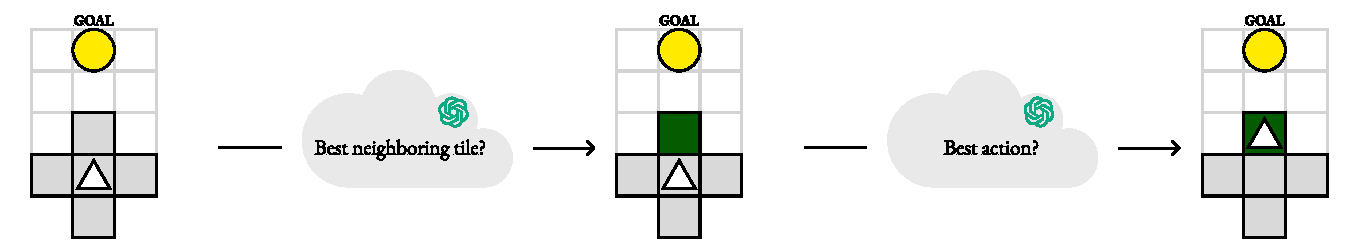
\includegraphics[width=\textwidth]{images/agent_development/extra.pdf}
  \caption{Two-steps decision making example}
  \label{fig:extra}
\end{figure}
\vspace{7mm}

This method effectively reframed the problem from a complex, global pathfinding
challenge into a series of simpler, localized decisions. We hypothesized that
this decomposition would improve performance by reducing the cognitive load on
the LLM and allowing it to focus on smaller, well-defined tasks.

However, despite these modifications, the results did not align with our expectations.
The primary issue was that if the agent misidentified the best neighboring tile
by choosing a position that actually increased the distance to the goal, then even
a perfectly chosen direction would still lead to suboptimal behavior.

Another significant factor was the role of uncertainty computation in the LLM response.
When relying on the raw output of the LLM (`Raw probability selection' in Section
\ref{sub:uncertainty_handling}), results were often inconsistent or outright incorrect.
To address this, we experimented also with the uncertainty-weighted random action
selection approach (`Weighted selection' in Section
\ref{sub:uncertainty_handling}), where decisions were influenced by the model's
confidence levels. Unfortunately, this introduced additional challenges, as interpreting
the results became even more complex.

Ultimately, this experiment underscored the limitations of LLM-based decision-making
in logistics scenarios where local optimizations must align with global
objectives. The agent's inability to consistently select the correct neighboring
tile demonstrated how small errors at the decision-making level could compound,
leading to inefficient or even counterproductive actions.

However, as we will explore in Chapter \ref{cha:results_discussion}, newer LLM
models exhibit notable improvements in our task, suggesting that continued advancements
in the technology may help overcome these challenges and enhance overall performance
in complex logistics tasks.
  \chapter{Data Collection}
\label{cha:data_collection}

In this chapter, we provide a comprehensive account of the data collection process
that underpins our experiments. We detail the key steps involved in designing, implementing,
and refining our methodology, with a particular focus on the construction and optimization
of the prompts used to interact with the Large Language Model.

We begin by presenting the core prompts utilized in our study, describing their
specific applications within each experimental setup. Following this, we outline
the rationale behind our prompt design decisions, grounding our choices in relevant
literature and highlighting key findings from previous research that informed our
approach.

Finally, we introduce the structure of our experimental evaluations, including the
generation of specialized heatmaps designed to illustrate the agent's uncertainty
in action selection. These visualizations provide valuable insights into the
model's decision-making process, highlighting both its generative strengths and areas
for further refinement.

\section{Prompts}
\label{sec:prompts}

This section provides a general overview of the prompts used in our experiments,
while the following one (Section \ref{sec:prompt_creation_choices}) will detail the
specific choices behind each specific part of them.

Our prompts were designed to be both concise and comprehensive, ensuring they
effectively guided the model in generating appropriate next-step actions. The core
idea was to elicit responses that incrementally moved the agent toward its objective,
either picking up or delivering a parcel, while minimizing ambiguity in the instructions.

The two primary prompts used in our study are:
\begin{itemize}
  \item Pickup prompt: guiding the agent to retrieve a parcel from a specified
    location;

  \item Delivery prompt: prompting the agent to transport the parcel to its
    designated drop-off point.
\end{itemize}

Each prompt was carefully structured to provide relevant contextual information while
avoiding unnecessary complexity that could dilute the model's focus.

\subsection{Pickup prompt}
\label{sub:pickup_prompt}

The Pickup prompt (Listing \ref{lst:pickup_prompt}) was used to evaluate the
model's ability to generate actions in the \emph{pickup} scenario. In this setup,
the agent was tasked with picking up a parcel from a specific location on the map.
The prompt provided the agent with the map information, including the map dimensions,
the location of the parcel, and the agent's current position.

The model was then asked to determine the optimal next action that would bring the
agent one step closer to the parcel.

\begin{codewindow}
  [Text] \lstset{style=promptstyle, language=prompt, caption={Pickup prompt used in the experiments},
  label={lst:pickup_prompt}} \begin{lstlisting}
You are a delivery agent in a web-based delivery game where the map is a matrix
I am going to give you the raw information I receive from the server and the possible actions.
Map width: {width}
Map height: {height}
Tiles are arranged as {height} rows in {width} columns:
{tiles}
The parcel you need to take is in the spot ({parcelX}, {parcelY}).
You are on the spot ({agentX}, {agentY}).
The actions you can do ONLY if the next tile is available are:
U) move up
D) move down
L) move left
R) move right
T) take the parcel that is in your tile
S) ship a parcel (you must be in a delivery tile)

Your final goal is to go to a tile with the parcel and (T)ake it, I need the best action that will get you there.
Don't explain the reasoning and don't add any comment, just provide the action's letter.
What is your next action?
\end{lstlisting}
\end{codewindow}

\subsection{Deliver prompt}
\label{sub:deliver_prompt}

The Delivery Prompt (Listing \ref{lst:deliver_prompt}) was structured to evaluate
the model's ability to navigate toward a designated drop-off location. Unlike
the Pickup Prompt, where the parcel's position was explicitly provided, the
delivery prompt required the LLM to infer the delivery destination from the map
description. The model was then asked to determine the best next action to move toward
the inferred delivery location.

\begin{codewindow}
  [Text] \lstset{style=promptstyle, language=prompt, caption={Deliver prompt used in the experiments},
  label={lst:deliver_prompt}} \begin{lstlisting}
You are a delivery agent in a web-based delivery game where the map is a matrix
I am going to give you the raw information I receive from the server and the possible actions.
Map width: {width}
Map height: {height}
Tiles are arranged as {height} rows in {width} columns:
{tiles}
You are on the spot ({agentX}, {agentY}).
The actions you can do are:
U) move up
D) move down
L) move left
R) move right
T) take the parcel that is in your tile
S) ship a parcel (you must be in a delivery tile)

You have a parcel to ship, your final goal is to go to the delivery zone (delivery = true) and (S)hip the parcel, I need the best action that will get you there.
Don't explain the reasoning and don't add any comment, just provide the action's letter.
What is your next action?
\end{lstlisting}
\end{codewindow}

\section{Prompt Creation Choices}
\label{sec:prompt_creation_choices}

This section outlines the key considerations that guided the construction of our
prompts (commonly referred to as \textbf{Prompt Engineering}). We describe the reasoning
behind specific design choices, following the sequence in which they appear in
the prompt. For clarity, we use the Pickup Prompt (Listing \ref{lst:pickup_prompt})
as a reference.

\subsection{Role Prompting}
Assigning specific roles or personas to Large Language Models within prompts, known
as ``role prompting," has been shown to enhance their performance on various tasks.
This technique involves instructing the model to assume a particular identity, such
as a ``math professor" or ``geographer," to guide its responses more effectively.
The concept of role prompting has been explored in several studies.

For instance, the paper `Better Zero-Shot Reasoning with Role-Play Prompting' by
Kong et al. \cite{kong2024betterzeroshotreasoningroleplay} demonstrated that strategically
designed role-play prompts can significantly improve LLMs' reasoning abilities
across diverse benchmarks.

Similarly, `Role-Play Zero-Shot Prompting with Large Language Models for Open-Domain
Human-Machine Conversation' by Njifenjou et al.
\cite{njifenjou2024roleplayzeroshotpromptinglarge} investigated the use of role-play
prompts to enhance conversational agents' performance without additional fine-tuning.

In our experiments, we employed role prompting to encourage the model to adopt
the persona of a \emph{delivery agent}, thereby focusing its attention on the
task at hand. By framing the prompts in this manner, we aimed to guide the model's
responses towards generating coherent and contextually relevant actions.

\subsection{Map Encoding to Reduce Attention Sparsity}

One of our primary concerns was that the map included in the prompt might take up
too much space, which could lead to an excessively sparse distribution of
attention. This could result in the model not properly focusing on crucial aspects
of the input. At the same time, we wanted to maintain a minimal and flexible approach
to map handling. Our goal was to ensure that the system would continue
functioning even if the format of the map-providing function were to change
unexpectedly. As discussed in Section \ref{sub:our_task}, this design decision
was made to simulate an unpredictable and rapidly changing environment.

To address this concern, we first aimed to understand how the model processed map-related
information. Ideally, we would have examined the models' attention scores
directly, but unfortunately, OpenAI's API does not provide access to these
scores. As a result, we had to rely on a qualitative analysis instead. To achieve
this, we leveraged BERT, another Transformer-based architecture, to visualize
attention patterns in our original prompt. The results revealed that a significant
portion of the models's attention was focused on tokens related to JSON syntax rather
than the meaningful content of the prompt itself. This suggested that structural
elements, rather than semantic information, were drawing a disproportionate
amount of attention.

Based on this observation, we attempted to reduce the presence of JSON syntax within
the prompt while preserving the essential information. We then repeated the same
attention analysis using this modified version. The results showed a shift in the
distribution of attention, even if the two prompts contained virtually the same
information. Specifically, when we examined the tokens receiving the highest
attention — excluding punctuation, as well as the special starting and ending tokens
— we found that in the original prompt, only 23 out of the top 50 tokens were
meaningful words. In contrast, in the revised prompt, this number increased to 31
out of 50, indicating a more focused attention on relevant content.

For this test, we used an older version of the ``Pickup prompt", which is explained
in detail in Section \ref{sec:second_approach}, with a small $2 \times 5$ map. As
demonstrated in Table \ref{tab:prompt_comparison}, the revised version of the
prompt not only contained more words in the top 50 tokens, but also explicitly included
the term \textbf{pickup}, which was the goal of the task. Notably, this term was
entirely absent from the top attention-receiving tokens in the initial prompt.

\begin{table}[ht]
  \centering
  \begin{tabular}{|c|c|}
    \hline
    \textbf{Old Prompt} & \textbf{New Prompt} \\
    \hline
    game                & game                \\
    reasoning           & parcel              \\
    parcel              & reasoning           \\
    parcel              & i                   \\
    score               & actions             \\
    response            & you                 \\
    parcel              & if                  \\
    tile                & parcel              \\
    i                   & moves               \\
    if                  & height              \\
    you                 & width               \\
    response            & score               \\
    loop                & ship                \\
    comment             & tile                \\
    information         & loop                \\
    actions             & information         \\
    and                 & choosing            \\
    ship                & you                 \\
    and                 & \textbf{pickup}     \\
    server              & and                 \\
    you                 & you                 \\
    choosing            & parcel              \\
    using               & and                 \\
                        & server              \\
                        & information         \\
                        & and                 \\
                        & ship                \\
                        & explain             \\
                        & using               \\
                        & reward              \\
                        & name                \\
    \hline
  \end{tabular}
  \caption{Comparison of Old and New Prompts}
  \label{tab:prompt_comparison}
\end{table}

To further analyze the impact of this change, we collected attention scores from
both the old and new prompt versions. We then removed the tokens corresponding
to the map representation in both prompts and plotted the difference between the
attention in the remaining common 264 tokens. The resulting visualization is presented
in Figure \ref{fig:difference} as the difference between \emph{old prompt
attention} and \emph{new prompt attention}. Interpreting this figure is not
entirely straightforward, and we acknowledge that it is unclear to what extent this
analysis can serve as a direct proxy for a GPT-based model. However, one noticeable
trend is that the diagonal elements exhibit a lower value (indicated by the
presence of purple and dark blue regions), indicating that the \emph{new prompt}
received more attention than the \emph{old prompt}. Meanwhile, most of the
remaining areas show a delta close to zero (represented in aqua blue), suggesting
that the changes we introduced led to a redistribution of attention without introducing
excessive noise or unintended biases. While this number does not have a direct
interpretative meaning, for completeness, we note that the total sum of the
difference matrix is about $- 15.34476$, indicating more attention in the new version
of the prompt.

\begin{figure}[ht!]
  \centering
  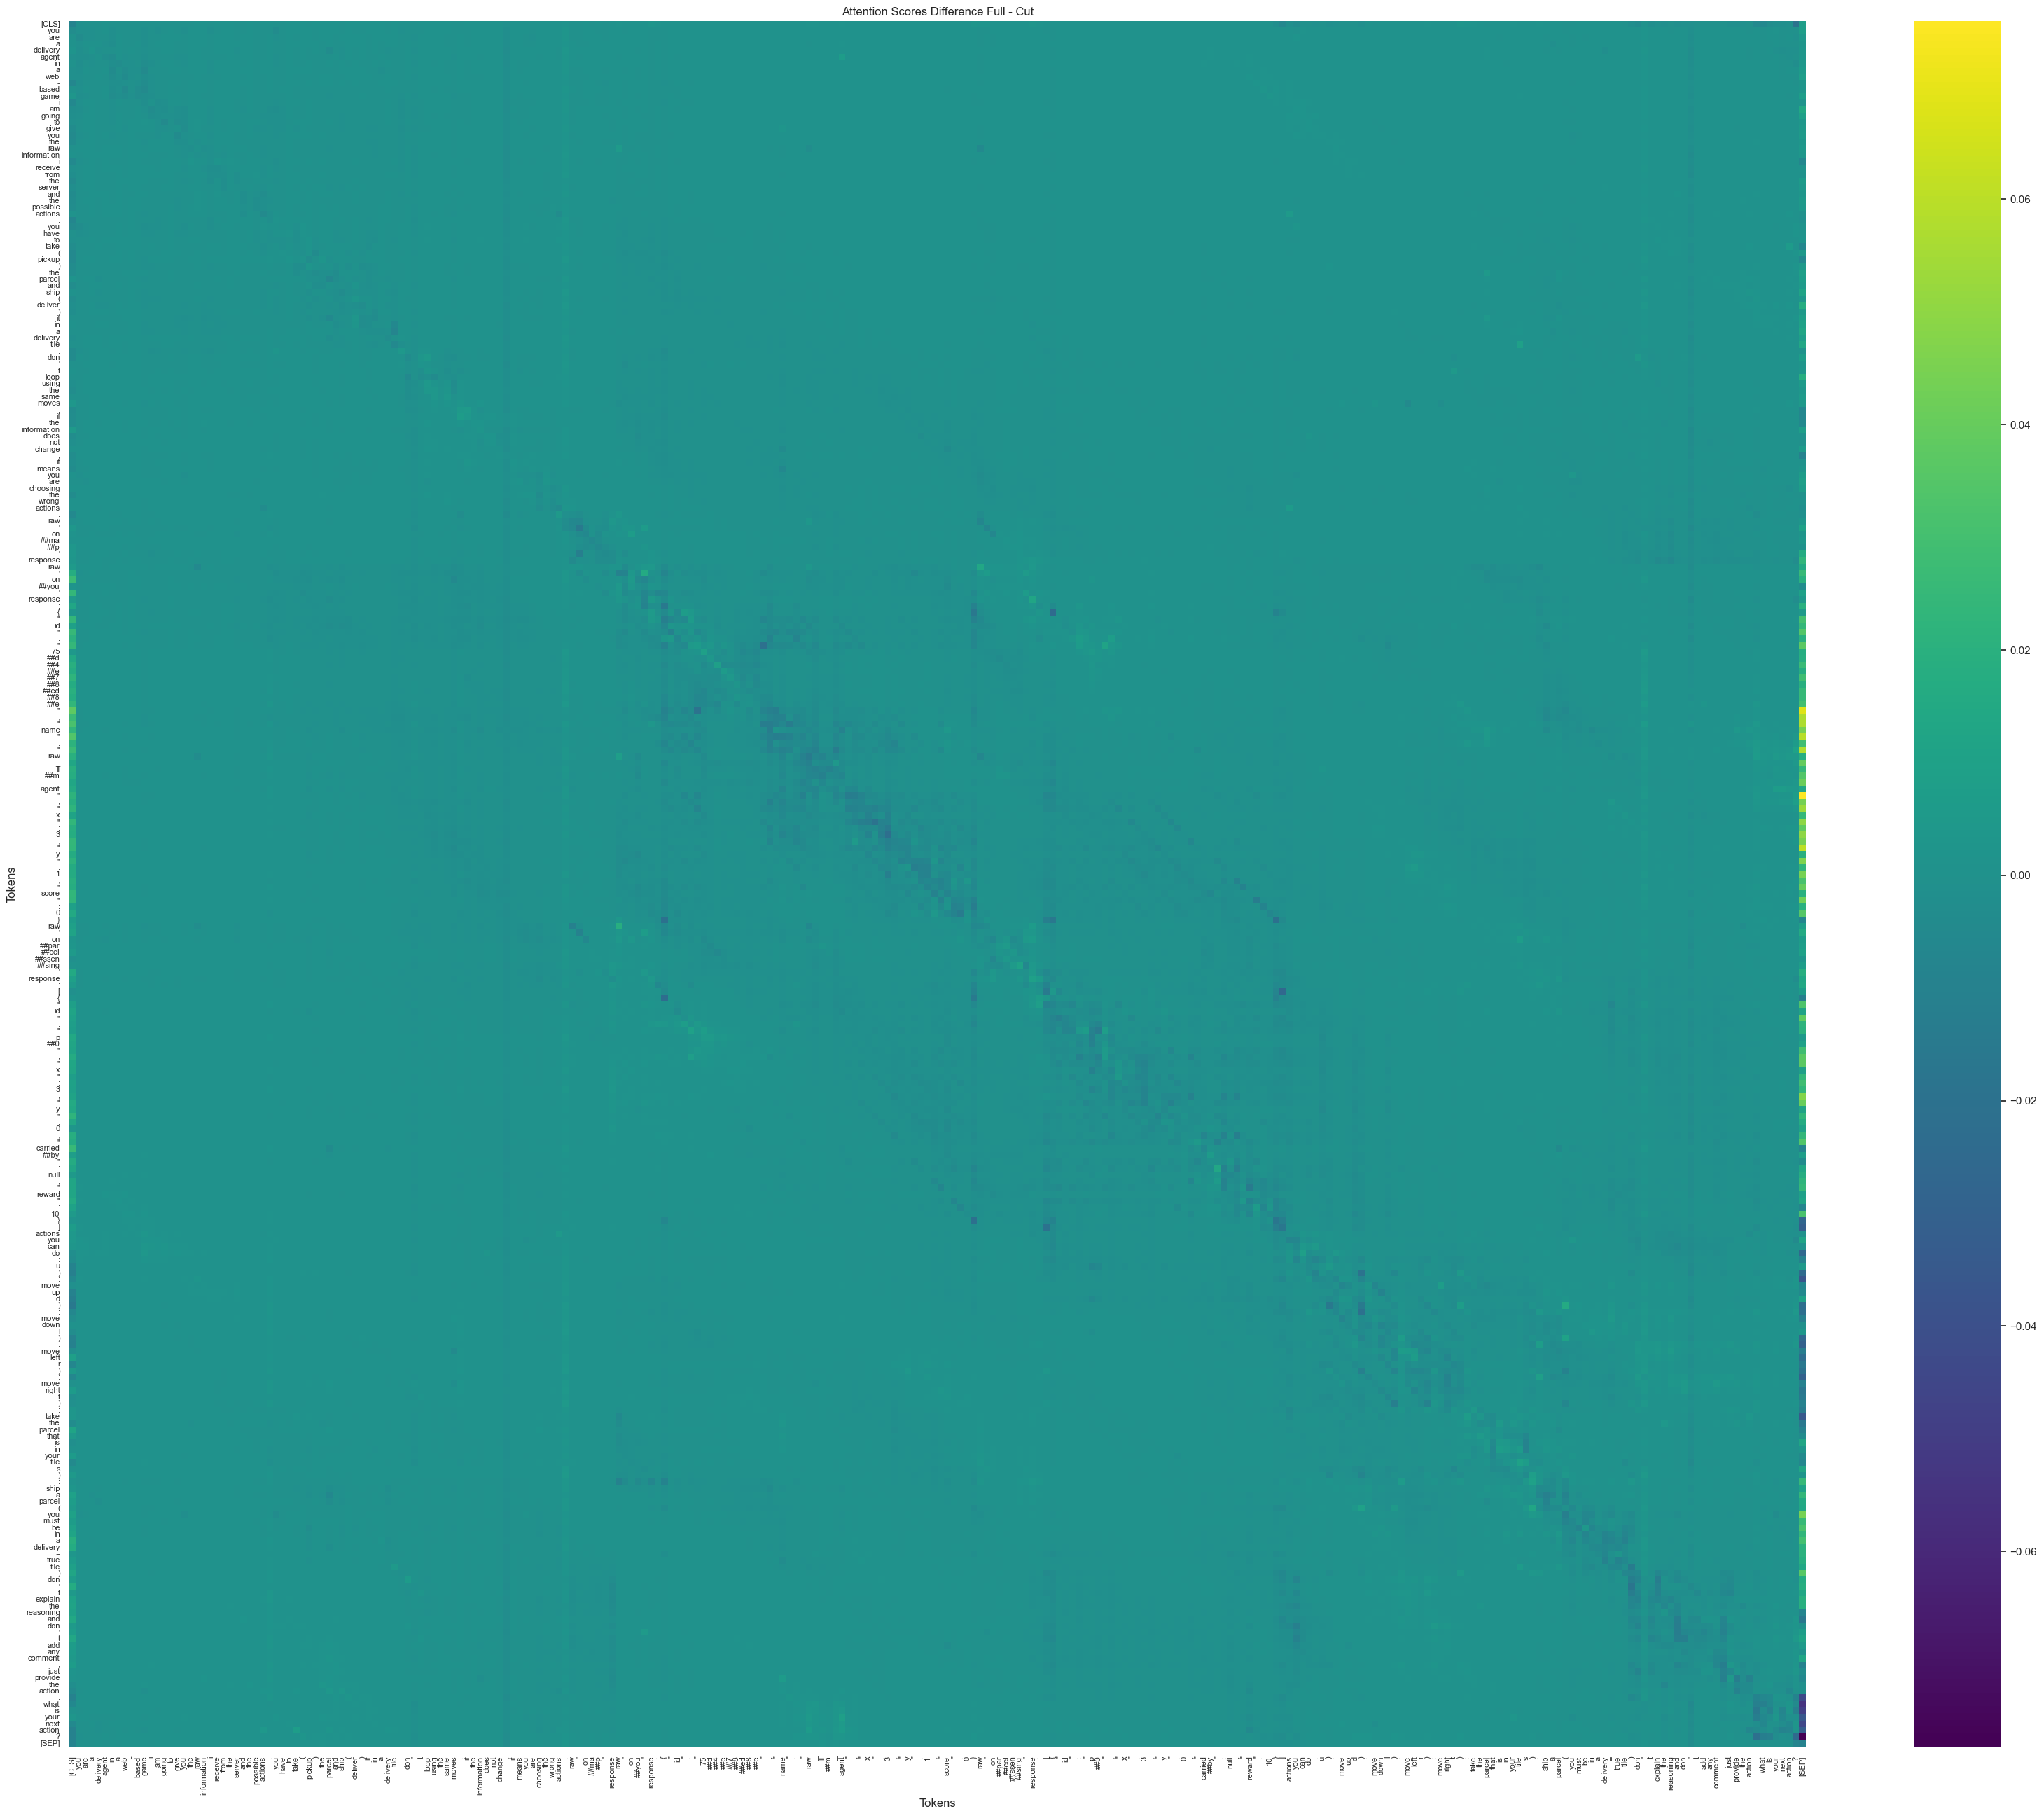
\includegraphics[width=0.8\textwidth]{images/data_collection/difference.png}
  \caption{Attention Difference between Old and New Prompts 264 common tokens. Full
  resolution available in the repository \cite{projectrepo}.}
  \label{fig:difference}
\end{figure}

\subsubsection{Emerging behavior: encoded question decoded answer}

Another strategy we explored to reduce the space occupied by the map in the prompt
was to encode it. Our goal was to compress the map representation while ensuring
that the model could still understand the relevant information.

A relevant study on this topic is presented in the paper `LLMs Can Understand Encrypted
Prompt: Towards Privacy-Computing Friendly Transformers' by Xuanqi Liu and Zhuotao
Liu\cite{liu2023llmsunderstandencryptedprompt}. The authors of this paper aimed to
preserve user privacy by encrypting prompts before sending them to a language model.
Their findings demonstrated that the model was able to comprehend and respond
appropriately to encrypted prompts. This suggested that LLMs possess an inherent
ability to process encoded text meaningfully.

Inspired by these results, we conducted an experiment to determine whether a
similar encoding approach could be used to reduce the space occupied by the map
while preserving its usability within the prompt. Specifically, we investigated
whether the model could still interpret a compressed version of the map if it
were encoded.

\vspace{5mm}
\begin{figure}[ht!]
  \centering
  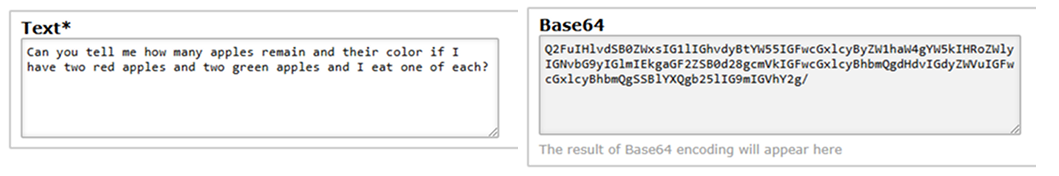
\includegraphics[width=0.98\textwidth]{images/data_collection/texttob64.png}
  \caption{Base64 encoding of a sample text}
  {\emph{Source: base64.guru}\footnotemark} \label{fig:texttob64}
\end{figure}
\footnotetext{\url{https://base64.guru/converter/encode/text}}
\vspace{5mm}

To validate this, we first examined the model's ability to process encoded
prompts by testing a simple case. As shown in Figure \ref{fig:b64gpt}, the model
successfully understood the meaning of the question ``Can you tell me how many
apples remain and their color if I have two red apples and two green apples and
I eat one of each?" even when the entire prompt was encoded in BASE64 (see Figure
\ref{fig:texttob64}). Notably, the model did not generate a decoding function
before answering. Instead, it directly processed the encoded prompt and returned
a response in plain English, demonstrating its ability to work with BASE64-encoded
text.

\begin{figure}[ht!]
  \centering
  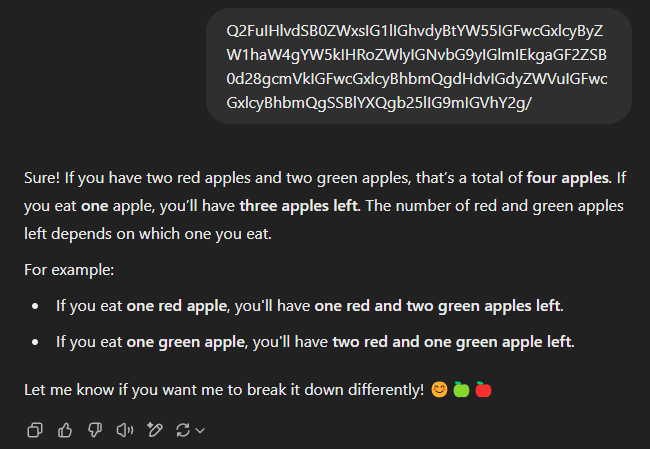
\includegraphics[width=0.66\textwidth]{images/data_collection/b64gpt.png}
  \caption{GPT-4o-mini response to a BASE64-encoded question}
  {\emph{Source: GPT-4o-mini via OpenAI web interface}} \label{fig:b64gpt}
\end{figure}

Encouraged by these results, we attempted to apply a similar encoding strategy to
the map representation while also aiming to reduce the number of characters in the
prompt. Our hypothesis was that reducing the character count would also reduce
the number of tokens, thereby improving attention efficiency.

To test this, we implemented a two-step encoding process in Python, as outlined in
Listing \ref{lst:double_enc}:
\begin{enumerate}
  \item First, we compressed the map using the \texttt{zlib} library and its Deflate
    algorithm \footnote{\url{https://en.wikipedia.org/wiki/Deflate}} to minimize
    its size;

  \item Next, we encoded the compressed output in BASE64 \footnote{\url{https://en.wikipedia.org/wiki/Base64}}
    using the \texttt{base64} library;

  \item Finally, we inserted this doubly encoded map into the prompt.
\end{enumerate}

\vspace{5mm}
\begin{codewindow}
  [Python Code] \lstset{style=pythonstyle, language=Python, caption={Example of double encoding algorithm},
  label={lst:double_enc}} \begin{lstlisting}
[...]

input_string = MAP
compressed_data = zlib.compress(input_string.encode('utf-8'))
compressed_base64 = base64.b64encode(compressed_data).decode('utf-8')

[...]
\end{lstlisting}
\end{codewindow}
\vspace{5mm}

While this method did succeed in reducing the number of characters by
$\sim 65\%$, the results were not as expected in terms of model comprehension.
Unlike the case of simple BASE64 encoding, the LLM was no longer able to interpret
the prompt correctly. Instead, its responses typically fell into one of two categories:
\begin{itemize}
  \item The model would explicitly state that it recognized the input as an encrypted
    message and generate something similar to ``It seems you've provided a compressed
    string or encoded data. Could you clarify how you'd like to use or process
    this? If it's encoded text, I can try decoding it for you.";

  \item Alternatively, if instructed with the encryption method used on the text,
    the model would generate a Python function to decode the input before attempting
    to process it. Such a function would have been executed ``under the hood" to
    decrypt the message before processing.
\end{itemize}

Furthermore, although our approach successfully reduced the total number of
characters in the prompt, it did not achieve our ultimate objective.

We then tried only using the BASE64 encoding, but the number of character
actually increased rather than decreased as well as the number of tokens that
increased even more in percentage. This is because tokenization in LLMs is based
on common character sequences rather than individual characters. Encoding the
map disrupted these common patterns, leading to a tokenization process that resulted
in a higher overall token count. Consequently, the intended effect of reducing attention
sparsity was not achieved, as illustrated in Figure \ref{fig:lesscharmoretokens}.

\vspace{5mm}
\begin{figure}[ht!]
  \centering
  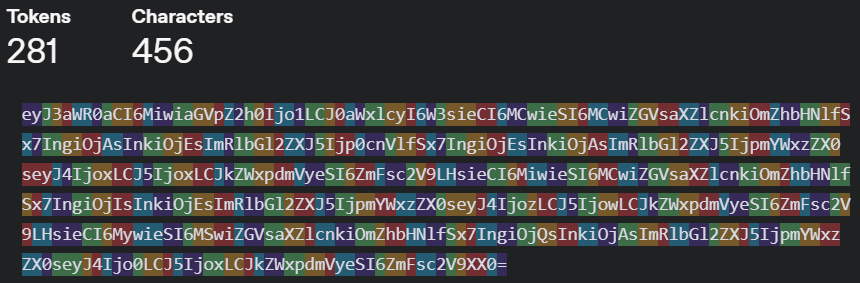
\includegraphics[width=0.66\textwidth]{
    images/data_collection/lesscharmoretokens.png
  }
  \caption{Tokenization of a BASE64-encoded text}
  {\emph{Source: GPT-4o tokenizer via OpenAI web interface}} \label{fig:lesscharmoretokens}
\end{figure}
\vspace{5mm}

In summary, while encoding techniques like BASE64 alone might be useful for
preserving meaning in certain contexts, our specific approach of compressing and
encoding the map did not lead to the desired efficiency gains. Instead, it introduced
additional computational overhead for the model, ultimately making this approach
ineffective for our purposes.

\subsection{Emerging behavior: math capabilities}

We also investigated the impact of including action-related information, such as
explicitly stating ``Going up increases your $X$ position by $1$" for every movement
action. It initially seemed like a promising way to guide the model's reasoning.
However, this conflicted with our overarching goal of keeping the system
adaptable rather than grounding it in a fixed environmental structure. Despite this,
we proceeded with the experiment to assess its impact.

Interestingly, we observed that the model's performance in navigation tasks was unexpectedly
strong, even to the point of raising concerns about potential shortcuts. To further
investigate, we conducted a follow-up test in which we entirely removed the map
from the prompt. As result, the model still produced correct answers by
seemingly ignoring any extraneous details and reducing the problem to simple
arithmetic. It recognized that if the starting position was \texttt{(4,2)} and
the goal was at \texttt{(0,0)}, the necessary movement was simply decreasing
\texttt{X} by 4 and \texttt{Y} by 2. This behavior demonstrated that the model
could abstract away the spatial representation and ``cheating'' by operating
purely on mathematical reasoning.

This finding aligns with existing research on the emergent mathematical
reasoning capabilities of large language models. For example, Wei et al. highlight
how LLMs exhibit ``emergent abilities", capabilities that do not appear in smaller
models but spontaneously manifest as model scale increases \cite{wei2022emergentabilitieslargelanguage}.
Among these abilities, arithmetic and mathematical reasoning are particularly notable,
suggesting that LLMs can generalize numerical patterns without explicit training
for such tasks. Our experiment provides anecdotal evidence supporting this:
rather than relying on the environmental constraints provided in the prompt, the
model instinctively leveraged its inherent mathematical capabilities to deduce the
necessary movements. Ultimately, given this behavior, we abandoned the idea of
including the results of the actions in the prompt.

\subsection{Question Structure}
\label{sub:question_structure}

A summarized example of a prompt used in the paper \emph{Robots That Ask For
Help: Uncertainty Alignment for Large Language Model Planners}
\cite{ren2023robotsaskhelpuncertainty} can be seen in Listing
\ref{lst:knowno_prompt}. This prompt has been taken directly from the example available
in their interactive demo\footnote{\url{https://tmp.com}}, which is accessible online.
The prompt follows a structured approach that allows the language model to
process information about the environment, understand the task, and select the
best action from a predefined set of choices.

Since we applied the same uncertainty analysis to the model's responses, we opted
to maintain a similar structure for our prompts.

\vspace{5mm}
\begin{codewindow}
  [Text] \lstset{style=promptstyle, language=Prompt, caption={Prompt from `Robots that ask for Help' paper},
  label={lst:knowno_prompt}} \begin{lstlisting}
You are a robot operating in an office kitchen. You are in front of a counter with two closed drawers, a top one and a bottom one. There is also a landfill bin, a recycling bin, and a compost bin.

On the counter, there is an energy bar, a banana, and a microwave.
Put the snack next to the microwave.

A) pick up the energy bar and put it next to the microwave
B) pick up the banana and put it next to the energy bar
C) pick up the banana and put it next to the microwave
D) pick up the energy bar and put it next to the banana

Which option is correct? Answer with a single letter.
\end{lstlisting}
\end{codewindow}
\vspace{5mm}

\subsubsection{Structure of the Paper's Prompt}

The structure of this prompt follows a well-defined pattern that guides the LLM's
reasoning process. It consists of the following key elements:

\begin{itemize}
  \item \textbf{Role and Environment Description}: The prompt starts by establishing
    the role of the model (a robot) and providing an overview of its working environment
    (an office kitchen);

  \item \textbf{Task Specification}: The next section provides a direct and unambiguous
    description of the task to be performed—in this case, placing a snack next
    to the microwave;

  \item \textbf{Action Choices}: A predefined list of actions (A, B, C, D, E) is
    presented, each corresponding to a possible decision. This format constrains
    the response space to just five choices;

  \item \textbf{Question and Response Constraint}: The prompt ends with a clear question
    that explicitly instructs the model to select an answer in a specific format
    (a single letter). This restriction allows for more structured uncertainty
    analysis as explained in Section \ref{ssub:tokens_log_probability}.
\end{itemize}

\subsubsection{Comparison with Our Approach}

Similarly, our prompt design follows the same structured approach: given our
task, our prompt structure aligns closely with the example above but incorporates
additional environmental details specific to our use case.

Our prompt structure consists of the following elements:

\begin{itemize}
  \item \textbf{Role and General Environment Description}: The prompt begins by defining
    the model's role (a delivery agent) and its operating context (a web-based
    delivery game);

  \item \textbf{Detailed Environment Specification}: Unlike the office kitchen scenario,
    our logistics task involves a structured map-based environment. Therefore,
    we explicitly include details such as:
    \begin{itemize}
      \item Map dimensions;

      \item Tile types and obstacles;

      \item Parcel location;

      \item Agent's current position.
    \end{itemize}

  \item \textbf{List of Possible Actions}: Instead of using letter-based choices
    (A, B, C, D, E), our prompt presents a set of movement and interaction
    commands:
    \begin{itemize}
      \item \textbf{U, D, L, R}: Move Up, Down, Left, Right;

      \item \textbf{T/S}: Pick up or deliver a parcel.
    \end{itemize}

  \item \textbf{Goal Definition and Question}: The prompt explicitly states the agent's
    goal, such as reaching a specific destination or delivering a parcel to an
    inferred goal tile. Additionally, the question is phrased to ensure a
    concise and structured response:
    \begin{quote}
      ``Your final goal is to [...] take the parcel. Just provide the action's
      letter. What is your next action?''
    \end{quote}
    This ensures that the model's response remains within the expected format,
    to evaluate the uncertainty in the same way as in the original paper.
\end{itemize}

A brief note: The letter ``T" for ``Take" was chosen instead of ``P" for ``Pickup"
because, in the initial version of the prompt (as discussed in Section \ref{sec:first_approach}),
$P$ was used to represent the parcel on the map. Similarly, ``S" for "Ship" was
selected, even though the server and other components refer to it as ``Deliver,"
as the letter $D$ was already assigned to the Down movement action.

\subsubsection{Multichoice Benchmarking}

Constraining the model's response to a predefined set of choices simplifies the
evaluation process. Moreover, multi-choice question answering is a widely
adopted method for benchmarking language models, as demonstrated in datasets such
as the Massive Multitask Language Understanding (MMLU) benchmark\footnote{\url{https://en.wikipedia.org/wiki/MMLU}}.
By enforcing a structured question format, we can systematically assess the
model's performance across different experimental conditions.

\subsection{Goal positioning}
\label{sub:goal_positioning}

As highlighted in the article `The Needle In a Haystack Test: Evaluating the Performance
of LLM RAG Systems'\cite{needleRAG}, LLMs exhibit a tendency to prioritize
information positioned at the beginning or end of a prompt, often overlooking details
embedded in the middle. To analyze this phenomenon, the researchers conducted an
experiment by inserting a unique "needle" token at different positions within a prompt
and measuring whether the model could successfully retrieve it in its response.
Their goal was to determine the optimal placement of information retrieved from
a retrieval-augmented generation system to maximize recall. Their findings revealed
that LLMs are most likely to recall information from the beginning and, to a
lesser extent, from the end, while details placed in the middle are more
frequently neglected.

This positional bias has significant implications for prompt engineering, especially
in structured queries. In our thesis, we follow a similar principle by positioning
the specific request at the end of the prompt. Understanding the model's
attention distribution allows us to optimize prompt design, ensuring that key details
receive the necessary emphasis to improve response accuracy and relevance.

Moreover, by placing the primary question at the end of the prompt, as well as all
the information that changes from a request to another, we can leverage OpenAI's
prompt caching capability of the API.

\subsubsection{Leveraging Prompt Caching}
\label{ssub:leveraging_prompt_caching} As can be seen in Listing
\ref{lst:deliver_prompt} and Listing \ref{lst:pickup_prompt}, the ``changing part"
of the prompt (mainly the position of the agent, but in case of a filtering of
the actions, also any updated list of possible actions), was placed at the end,
while the main static components, including the role and map, were positioned at
the top. This structure was the result of a literature analysis while it also takes
advantage of OpenAI's prompt caching API\footnote{\url{https://platform.openai.com/docs/guides/prompt-caching}}.

According to OpenAI's documentation, for any prompt exceeding 1000 tokens, only
the modified portion is recomputed, while the cached static portion remains unchanged.
This significantly improves efficiency by reducing computational overhead, resulting
in faster response times and lower operational costs.

The benefits of this approach are especially pronounced in the stateful version of
the agent, where the LLM receives the entire conversation history with each
request. In this case, caching allows the model to handle long, continuous interactions
without constantly reprocessing the entire history from scratch, making the
system much more scalable and responsive.

By structuring prompts in this manner, we ensure that also queries for a stateless
agent in a bigger environment or with more actions available (necessary to reach
the 1000 tokens count) can benefit from caching, leading to optimized
performance in a scenario that requires frequent API calls.

\section{Uncertainty Visualization}
\label{sec:uncertainty_visualization}

\begin{blockquote}
  A \textbf{heat map} (or heatmap) is a 2-dimensional data visualization
  technique that represents the magnitude of individual values within a dataset
  as a color. The variation in color may be by hue or intensity.

  [...]\\There are two main type of heat maps: spatial, and grid.
  \begin{itemize}
    \item A spatial heat map displays the magnitude of a spatial phenomena as color,
      usually cast over a map. In the image labeled "Spatial Heat Map Example,"
      temperature is displayed by color range across a map of the world. Color ranges
      from blue (cold) to red (hot).

    \item A grid heat map displays magnitude as color in a two-dimensional matrix,
      with each dimension representing a category of trait and the color
      representing the magnitude of some measurement on the combined traits from
      each of the two categories. For example, one dimension might represent
      year, and the other dimension might represent month, and the value
      measured might be temperature.
  \end{itemize}
  \emph{Source: Wikipedia\footnotemark}
\end{blockquote}
\footnotetext{\url{https://en.wikipedia.org/wiki/Heat_map}}

As stated in the definition above, heatmaps are a powerful tool for visualizing data,
allowing for a compact and intuitive representation of large datasets. In our case,
we employ heatmaps to capture and convey the uncertainty in the agent's decision-making
process at each position within the matrix. Specifically, the heatmaps encode
the probabilities assigned by the KnowNo framework to the various possible
actions.

The primary goal of these heatmaps is to provide a clear and structured means of
analyzing how the agent distributes probabilities over its available actions. By
mapping these probabilities onto a visual representation, we gain insights into
which areas of the matrix exhibit high certainty (where one action dominates)
and which regions display greater uncertainty (where multiple actions hold comparable
probabilities). These heatmaps serve as a diagnostic tool for evaluating the agent's
behavior, identifying patterns, and pinpointing potential areas for improvement in
future iterations.

More specifically, we utilize this visualization for two key aspects of our
analysis:

\begin{itemize}
  \item \textbf{Heatmaps}: To represent the probability distribution over the filtered
    list of actions. This means that after discarding actions with probabilities
    below the predefined threshold (as detailed in Section \ref{ssub:tokens_log_probability}),
    the heatmap displays the remaining probability assigned to the remaining actions
    (with the total percentage scaled back to 100\%);

  \item \textbf{Correctness Heatmaps}: To represent the overall probability assigned
    to the correct actions in each cell of the matrix. This allows us to measure
    how well the model aligns with the expected optimal behavior, providing a way
    to assess the agent's effectiveness in selecting appropriate actions.
\end{itemize}

These heatmaps are central to our data collection and analysis pipeline. By
systematically constructing and analyzing them, we can track how the agent's decision-making
evolves over time and across different configurations of the problem space. We
can also identify systematic behaviors, biases, or areas where the model
struggles, that we will analyze in Chapter \ref{cha:results_discussion}.

The final analysis will rely heavily on these heatmaps to provide a comprehensive
understanding of the agent's performance and behavior.

\subsection{Heatmaps}
\label{sub:heatmaps}

Heatmaps provide a visual representation of the probability distribution of
actions taken within each cell of the environment. By encoding probability values
as color intensities, these heatmaps offer an intuitive way to interpret the
model's decision-making process across the entire grid. Each cell in the heatmap
corresponds to a specific position in the environment, with colors indicating
the not-discarded actions in that location.

To generate these heatmaps, a specialized stateless agent systematically scans the
map, cell by cell, from the top-left to the bottom-right. At each position, it records
the probabilities assigned to each possible action. The collected data is then
stored in a JSON format, as shown below:

\begin{verbatim}
[
  {
    "x":0,"y":0,
    "values":[
      ["R",true,0.9869068698680659],
      ["D",false,0.004691684231979342],
      ["U",false,0.002214120084731493],
      ["S",false,0.0021401869314925225],
      ["L",false,0.002023569441865407],
      ["T",false,0.002023569441865407]
      ]
  },
  ...
]
\end{verbatim}

In this format, each entry represents a specific cell identified by its coordinates
$(x,y)$. The \texttt{values} field contains a list of possible actions, each
represented by:
\begin{itemize}
  \item The action itself (e.g., ``R" for Right, ``D" for Down, etc.);

  \item A boolean value indicating whether the action was retained after filtering;

  \item The probability assigned to that action by the framework.
\end{itemize}
Once this data is collected, a Python script processes it to generate the final
heatmap, which visually encodes the probability distribution for each action.

An example of such a heatmap is shown in Figure \ref{fig:heatmap_example}. Only
the probability of the retained actions is displayed.

\begin{figure}[ht!]
  \centering
  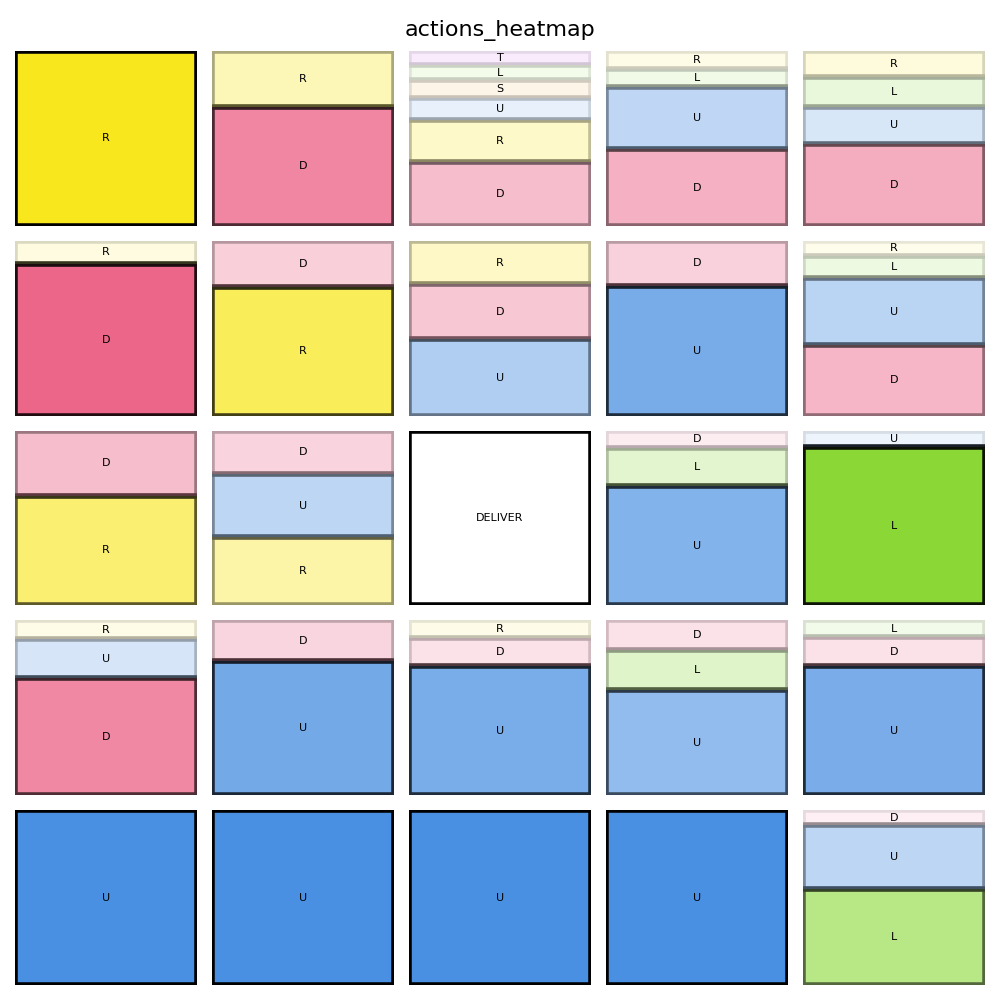
\includegraphics[width=0.8\textwidth]{
    images/data_collection/heatmap_example.png
  }
  \caption{Example of a heatmap generated for a $5 \times 5$ map}
  \label{fig:heatmap_example}
\end{figure}

To enhance interpretability, each action is represented using a distinct color:
\begin{itemize}
  \item Green: Left (L)

  \item Yellow: Right (R)

  \item Red: Down (D)

  \item Blue: Up (U)

  \item Purple: Take (T) (picking up a parcel)

  \item Orange: Ship (S) (delivering a parcel)
\end{itemize}
Additionally, the transparency (alpha value) of each color is adjusted based on
the probability of that action, allowing more probable actions to appear more prominently.

A total of 36 test cases have been conducted, and the resulting heatmaps are
stored in the repository under the following directory structure: \begin{verbatim}
../data_and_results/heatmap/heatmaps/MODEL/MAP/GOAL/GOAL_POSITION/
\end{verbatim}
where the last folder contains four files:
\begin{itemize}
  \item \texttt{actions\_heatmap.png}: the rendered heatmap referring to that specific
    test;

  \item \texttt{correctness\_heatmap.png}: the heatmap representing the probability
    of the correct actions that will be discussed in Section \ref{sub:correctness_heatmaps};

  \item \texttt{heatmap.json}: the raw data collected for the heatmap;

  \item \texttt{topX\_values.json}: statistics regarding the \texttt{correctness\_heatmap.png}
    that will be used in the final analysis in Chapter
    \ref{cha:results_discussion}.
\end{itemize}

This organizational structure guarantees that, for each map size, both pickup and
delivery goals are thoroughly tested to cover a wide range of scenarios.
Additionally, in certain cases, we have included other specific goals or prompts
to examine particular behaviors or edge cases of the agent. By incorporating these
varied test configurations, we ensure a comprehensive evaluation of the agent's
performance, which will provide valuable insights for analyzing the results in more
depth.

The location of the goals are varied across different test cases; the rationale
behind choosing ``which tile should be the goal'' will be discussed in Chapter
\ref{cha:results_discussion}.

\subsubsection{Example}

To better understand how to interpret these heatmaps, let us analyze a specific
case. Figure \ref{fig:heatmap_example} presents a heatmap generated for a $5 \times
5$ grid, where the agent's objective is to deliver a parcel at the center of the
map.

Consider the cell at coordinates $(2,1)$, which is positioned directly to the left
of the goal. This location is particularly interesting because, being adjacent to
the delivery point, the agent should ideally display a strong preference for
moving Right (R) to complete the task efficiently. The KnowNo framework produced
the following probability distribution for this cell:

\begin{verbatim}
  ...
  {
    "x": 2,
    "y": 1,
    "values": [
      ["R", true, 0.34148147866149986],
      ["U", true, 0.3185527747471083],
      ["D", true, 0.2173149034701972],
      ["T", false, 0.04243503226711094],
      ["L", false, 0.040951236117811166],
      ["S", false, 0.03926457473627248]
    ]
  },
  ...
\end{verbatim}

From this data, we can extract several key observations:
\begin{itemize}
  \item Dominant Actions: The three highest-probability actions at this cell are
    Right (R) with 34.14\%, Up (U) with 31.85\%, and Down (D) with 21.73\%. This
    indicates that while the model slightly favors moving Right, it still considers
    moving Up or Down as viable options;

  \item Discarded Actions: Actions such as Left (L) (4.10\%), Take (T) (4.24\%),
    and Ship (S) (3.93\%) were assigned very low probabilities and subsequently filtered
    out by the KnowNo framework, meaning they were not considered in the final
    action selection process. This suggests that the model appropriately recognizes
    that moving left or attempting to interact with the parcel at this position is
    not optimal;

  \item Probability Normalization: After discarding the low-probability actions,
    the remaining three probabilities were rescaled to sum to 100\%. This renormalization
    ensures that the final action selection is based solely on the most relevant
    choices.
\end{itemize}

This example illustrates how the heatmap helps us diagnose the model’s decision-making
tendencies. Ideally, in this scenario, the probability of moving Right (R)
should be significantly higher, given that it is the only direct path to the goal.
However, the model also considers alternative movements, highlighting potential
limitations in its capabilities.

This example already highlights some potential limitations of the system, particularly
in terms of decision ambiguity when the agent is very near to the goal, which
will be further examined in Chapter \ref{cha:results_discussion}.

\subsection{Correctness Heatmaps}
\label{sub:correctness_heatmaps}

After constructing the action-probability heatmaps, we generate an additional
set of heatmaps that focus on correctness. These correctness heatmaps aim to evaluate
how well the model aligns with the expected optimal behavior by quantifying the probability
assigned to the correct actions at each position in the map.

To construct these correctness heatmaps, we start determining the set of correct
actions for each cell using a Python script similar to the one in Listing
\ref{lst:correctness_script}. This script systematically analyzes the spatial relationship
between each tile and the designated goal position, identifying which movements
(e.g., U, D, L, R) would bring the agent closer to the goal. The resulting list
of correct actions serves as the reference against which we measure the model's
decision-making accuracy.

\vspace{5mm}
\begin{codewindow}
  [Python Code] \lstset{style=pythonstyle, language=Python, caption={If statements to compute the correct actions for every cell},
  label={lst:correctness_script}} \begin{lstlisting}
for tile in tiles:
    delta_y = goal_y - tile['y']
    delta_x = goal_x - tile['x']
    correct_moves = []
    if delta_x > 0:
        correct_moves.append('D')
    if delta_x < 0:
        correct_moves.append('U')
    if delta_y > 0:
        correct_moves.append('R')
    if delta_y < 0:
        correct_moves.append('L')

    percentage = 0
    for value in tile['values']:
        if value[0] in correct_moves:   # value[0] is the letter
            percentage += value[2]      # value[2] is the probability

    total_percentage = sum([value[2] for value in tile['values']])
    percentage = percentage / total_percentage
\end{lstlisting}
\end{codewindow}
\vspace{5mm}

The correctness heatmap visually represents the proportion of probability assigned
to correct actions in each cell. This allows us to assess the model's
effectiveness in adhering to expected behavior and helps highlight areas where
the agent struggles to make optimal choices.

Figure \ref{fig:correctness_example} illustrates an example correctness heatmap
corresponding to the action probability heatmap shown earlier in Figure
\ref{fig:heatmap_example}.

\begin{figure}[ht!]
  \centering
  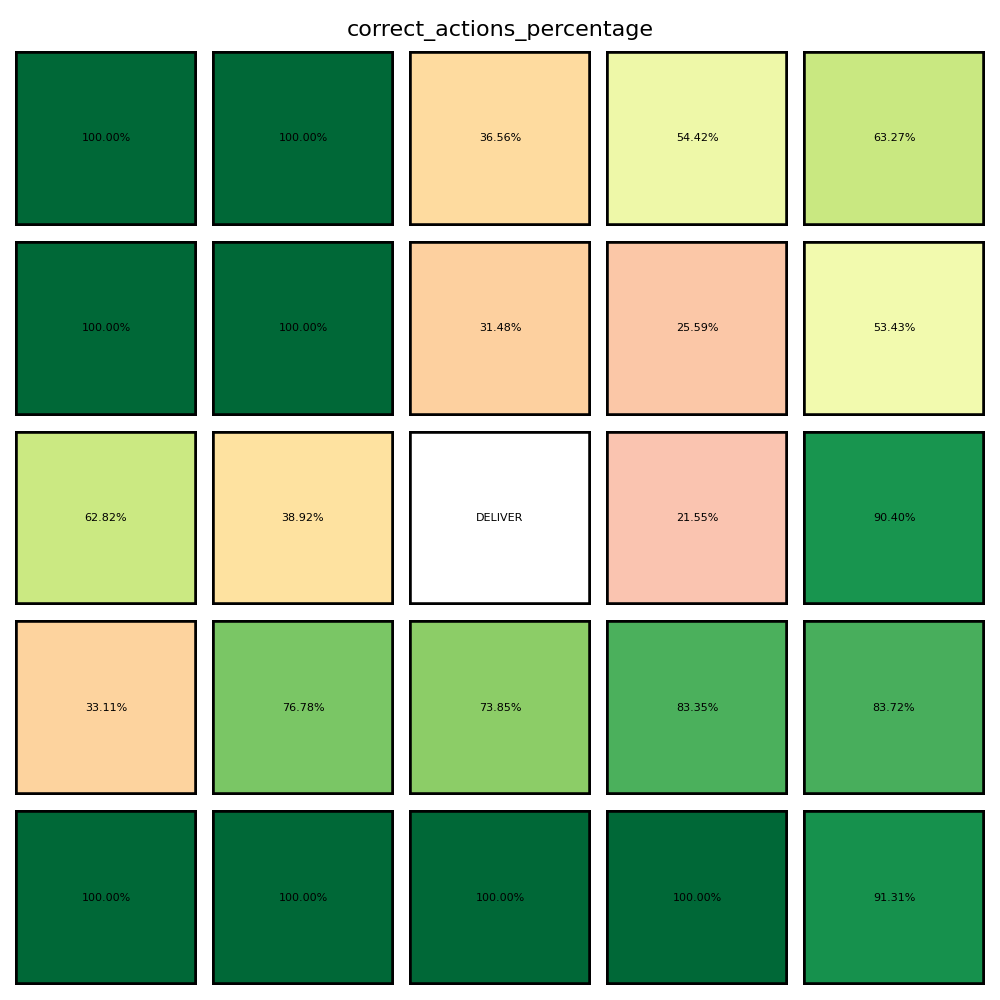
\includegraphics[width=0.8\textwidth]{
    images/data_collection/correctness_example.png
  }
  \caption{Example of a correctness heatmap generated for a $5 \times 5$ map}
  \label{fig:correctness_example}
\end{figure}

\subsubsection{Example}

To better understand the significance of the correctness heatmap, let's revisit the
previously analyzed cell at coordinates $(2,1)$, which is located directly to
the left of the goal position in a $5 \times 5$ grid.

To compute the correctness probability for this cell, we get the probability of the
correct action (Right) and normalize it against the total probability assigned to
retained actions.

\vspace{5mm}
\begin{codewindow}
  [Text] \lstset{style=promptstyle, language=Prompt, caption={Scaling of the probability after filtering},
  label={lst:percentage_compute}} \begin{lstlisting}
total_percentage = 0.34148 + 0.31855 + 0.21731 (= 0.87734)
percentage = 0.34148 / total_percentage (= 0.38922)
\end{lstlisting}
\end{codewindow}
\vspace{5mm}

Thus, if the agent selects an action randomly while weighting choices according to
their assigned probabilities (as described in Section
\ref{sub:uncertainty_handling}), in this case it would have a 38.92\% chance of choosing
the correct action, as shown in Listing \ref{lst:percentage_compute}.

This metric provides valuable insight into the model's decision-making
tendencies: while the model recognizes the correct action, it also considers
alternative actions with relatively high probability, indicating uncertainty in its
decision-making process.

By examining correctness heatmaps across different test cases, we can identify
patterns and inconsistencies in the model's behavior. These heatmaps help us pinpoint
areas where the model exhibits high confidence in correct actions and areas where
it is more uncertain or prone to errors.

Some key insights that can be derived from correctness heatmaps include:
\begin{itemize}
  \item High-confidence regions: Cells where the model assigns a near-total
    probability to correct actions indicate strong alignment with expected
    behavior;

  \item Uncertain regions: Areas with distributed probability mass among
    multiple actions suggest indecision, which could stem from ambiguous training
    data or suboptimal model reasoning;

  \item Error-prone zones: Cells where incorrect actions receive a significant
    portion of the probability mass highlight potential weaknesses in the model's
    decision-making.
\end{itemize}
These correctness heatmaps provide a structured way to assess the agent's
decision-making process, offering insights into how well it aligns with expected
behavior. By analyzing these visualizations, we can identify areas where the model
exhibits high confidence in correct actions and regions where it shows uncertainty
or inconsistencies. This analysis will be further explored in Chapter
\ref{cha:results_discussion}, where we examine the broader implications of these
findings.
  \chapter{Results Discussion}
\label{cha:results_discussion}

In this chapter, we analyze the results of our experiments, focusing on how the
agent performs in different maps and goals configuration to evaluate the agent's
ability to navigate the map and successfully complete its tasks. We examine how the
placement of goal tiles affects decision-making, assess whether the model
struggles with retrieving relevant information, and compare the performance in the
same slice of different maps.

Our primary objective is to evaluate the agent's ability to navigate the map and
successfully complete pickup and delivery tasks.

In tasks where the agent's goal is to pick up a parcel, the target tile
corresponds to the one containing the parcel. Conversely, in delivery tasks, the
goal tile is the specific location where the agent must deliver the parcel.

The placement of goal tiles within the game map was carefully designed to ensure
consistency and meaningful evaluation across both pickup and delivery tasks.
Specifically, we aimed to use the same goal tiles for both objectives, allowing
for direct comparisons between the two. In the pickup scenario, the goal is
always explicitly stated at the end of the prompt, making it immediately available
to the LLM. However, in the delivery scenario, the agent must retrieve the
delivery location from the provided map description, requiring it to process and
extract the relevant information effectively.

To evaluate how well the model handles goal retrieval, we selected three
distinct goal positions: the top-right, center, and bottom-right cells of the map.
These placements ensure that the goal appears in different parts of the map
description inside the prompt, allowing us to assess whether the ``needle in a haystack"
problem, as discussed in related literature, affects the model's ability to
locate and act on relevant information during the delivery task.

In the final section, we will discuss the different LLMs used in the agent's decision-making
process. As a general observation, GPT-3.5 performed worse compared to the more advanced
GPT-4o variants. Among the newer models, GPT-4o and GPT-4o-mini demonstrated similar
performance, with both outperforming GPT-3.5. Due to budget constraints, the
majority of our analysis was conducted using GPT-4o-mini, as it provides a cost-effective
yet high-quality alternative. However, our qualitative findings can be reasonably
extended to GPT-4o as well, given their comparable performance, and to all models
with similar performance and/or architecture. Each LLM call had an average input
size of approximately 250 tokens, with only a single token as output. The cost
per call was approximately \$0.000038 USD.

\section{Map Orientation}

In this section, we analyze the impact of map orientation on the agent's decision-making
process. Since the prompt did not explicitly reference any specific orientation,
the model had to infer it based solely on the provided map description and its training
data. By examining the model's outputs, we can determine its perceived orientation
of the map and assess whether any biases emerge.

To investigate this, we analyzed the data using two different origin conventions.
The raw data was structured with the $(0,0)$ coordinate in the top-left corner,
but we also transformed the map to simulate a bottom-left origin by adjusting
all coordinates accordingly. We then ran the agent in both configurations—one using
the original top-left origin and another using the simulated bottom-left origin—to
compare how the agent's actions varied under different map orientations.

As illustrated in Figure \ref{fig:orientation}, the heatmaps of the agent's
actions appear nearly identical, except for a 90-degree rotation. The small
differences between the two cases can be attributed to the way the data was
structured in the prompt, which may have influenced the model's text generation.

\begin{figure}[h]
  \centering
  \begin{minipage}[b]{0.45\textwidth}
    \centering
    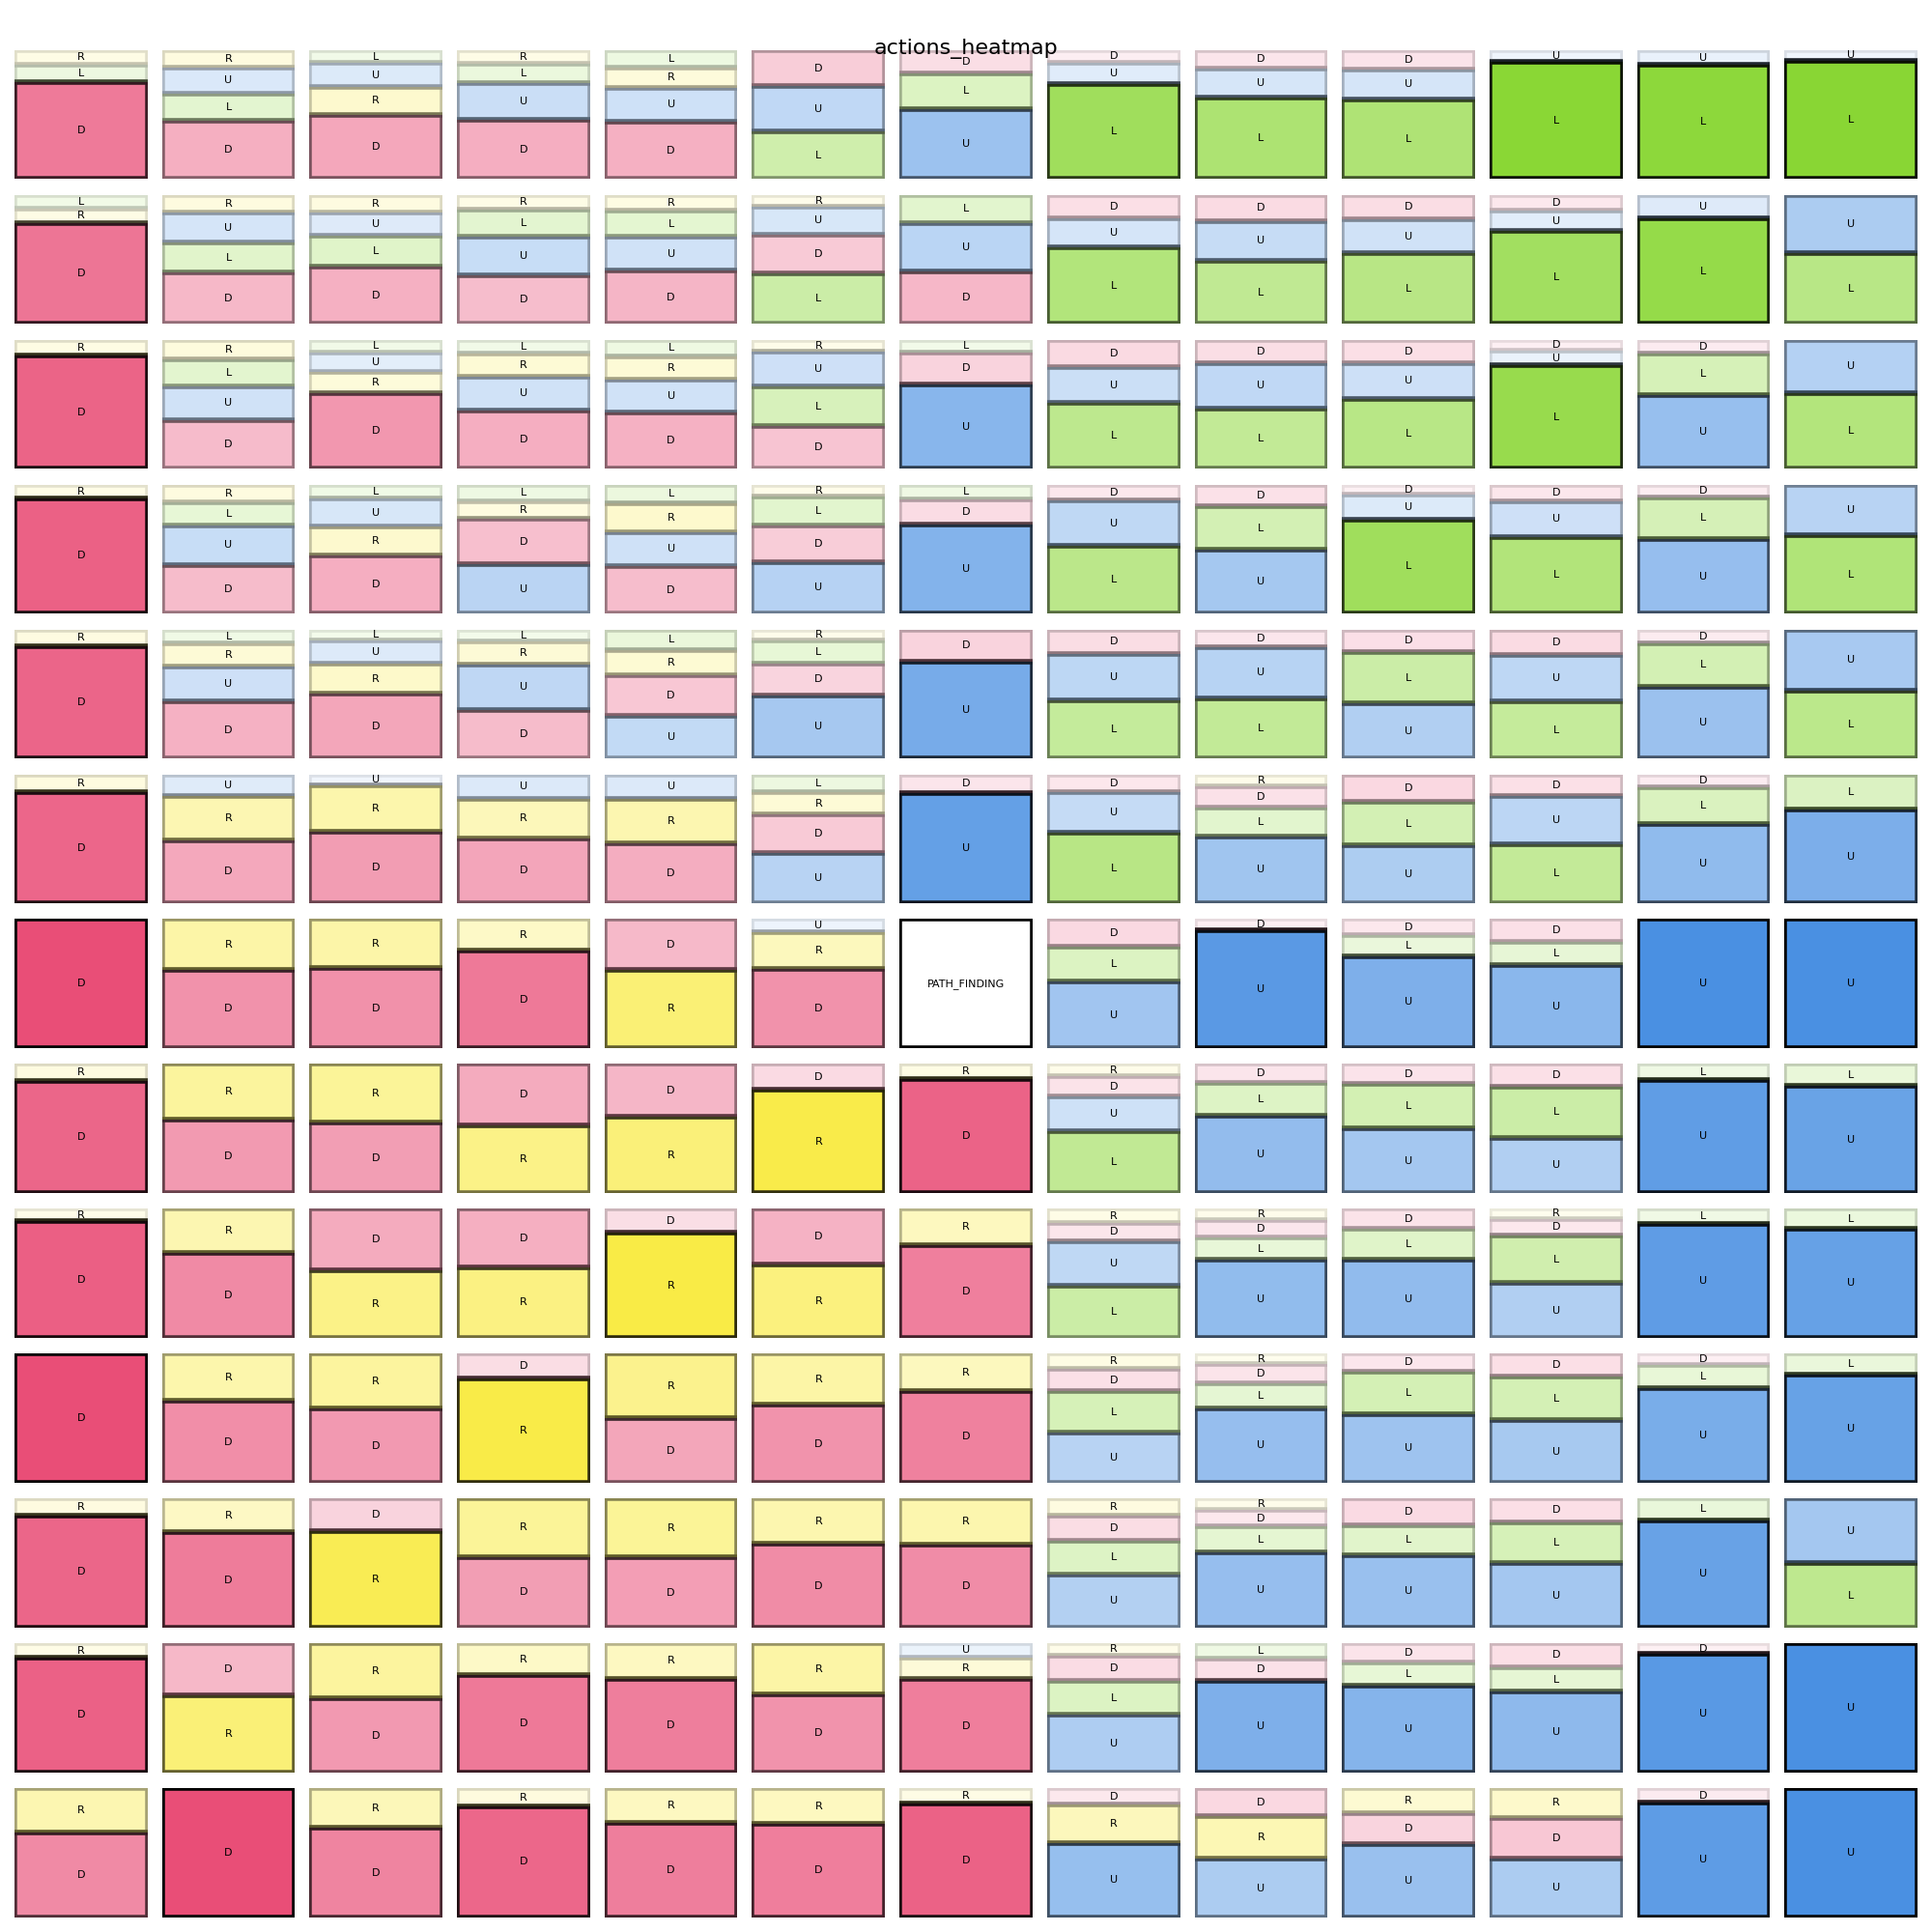
\includegraphics[width=\textwidth]{
      images/results_discussion/actions_heatmapBL.png
    }
    \caption{Bottom Left Orientation}
    \label{fig:heatmapBL}
  \end{minipage}
  \hfill
  \begin{minipage}[b]{0.45\textwidth}
    \centering
    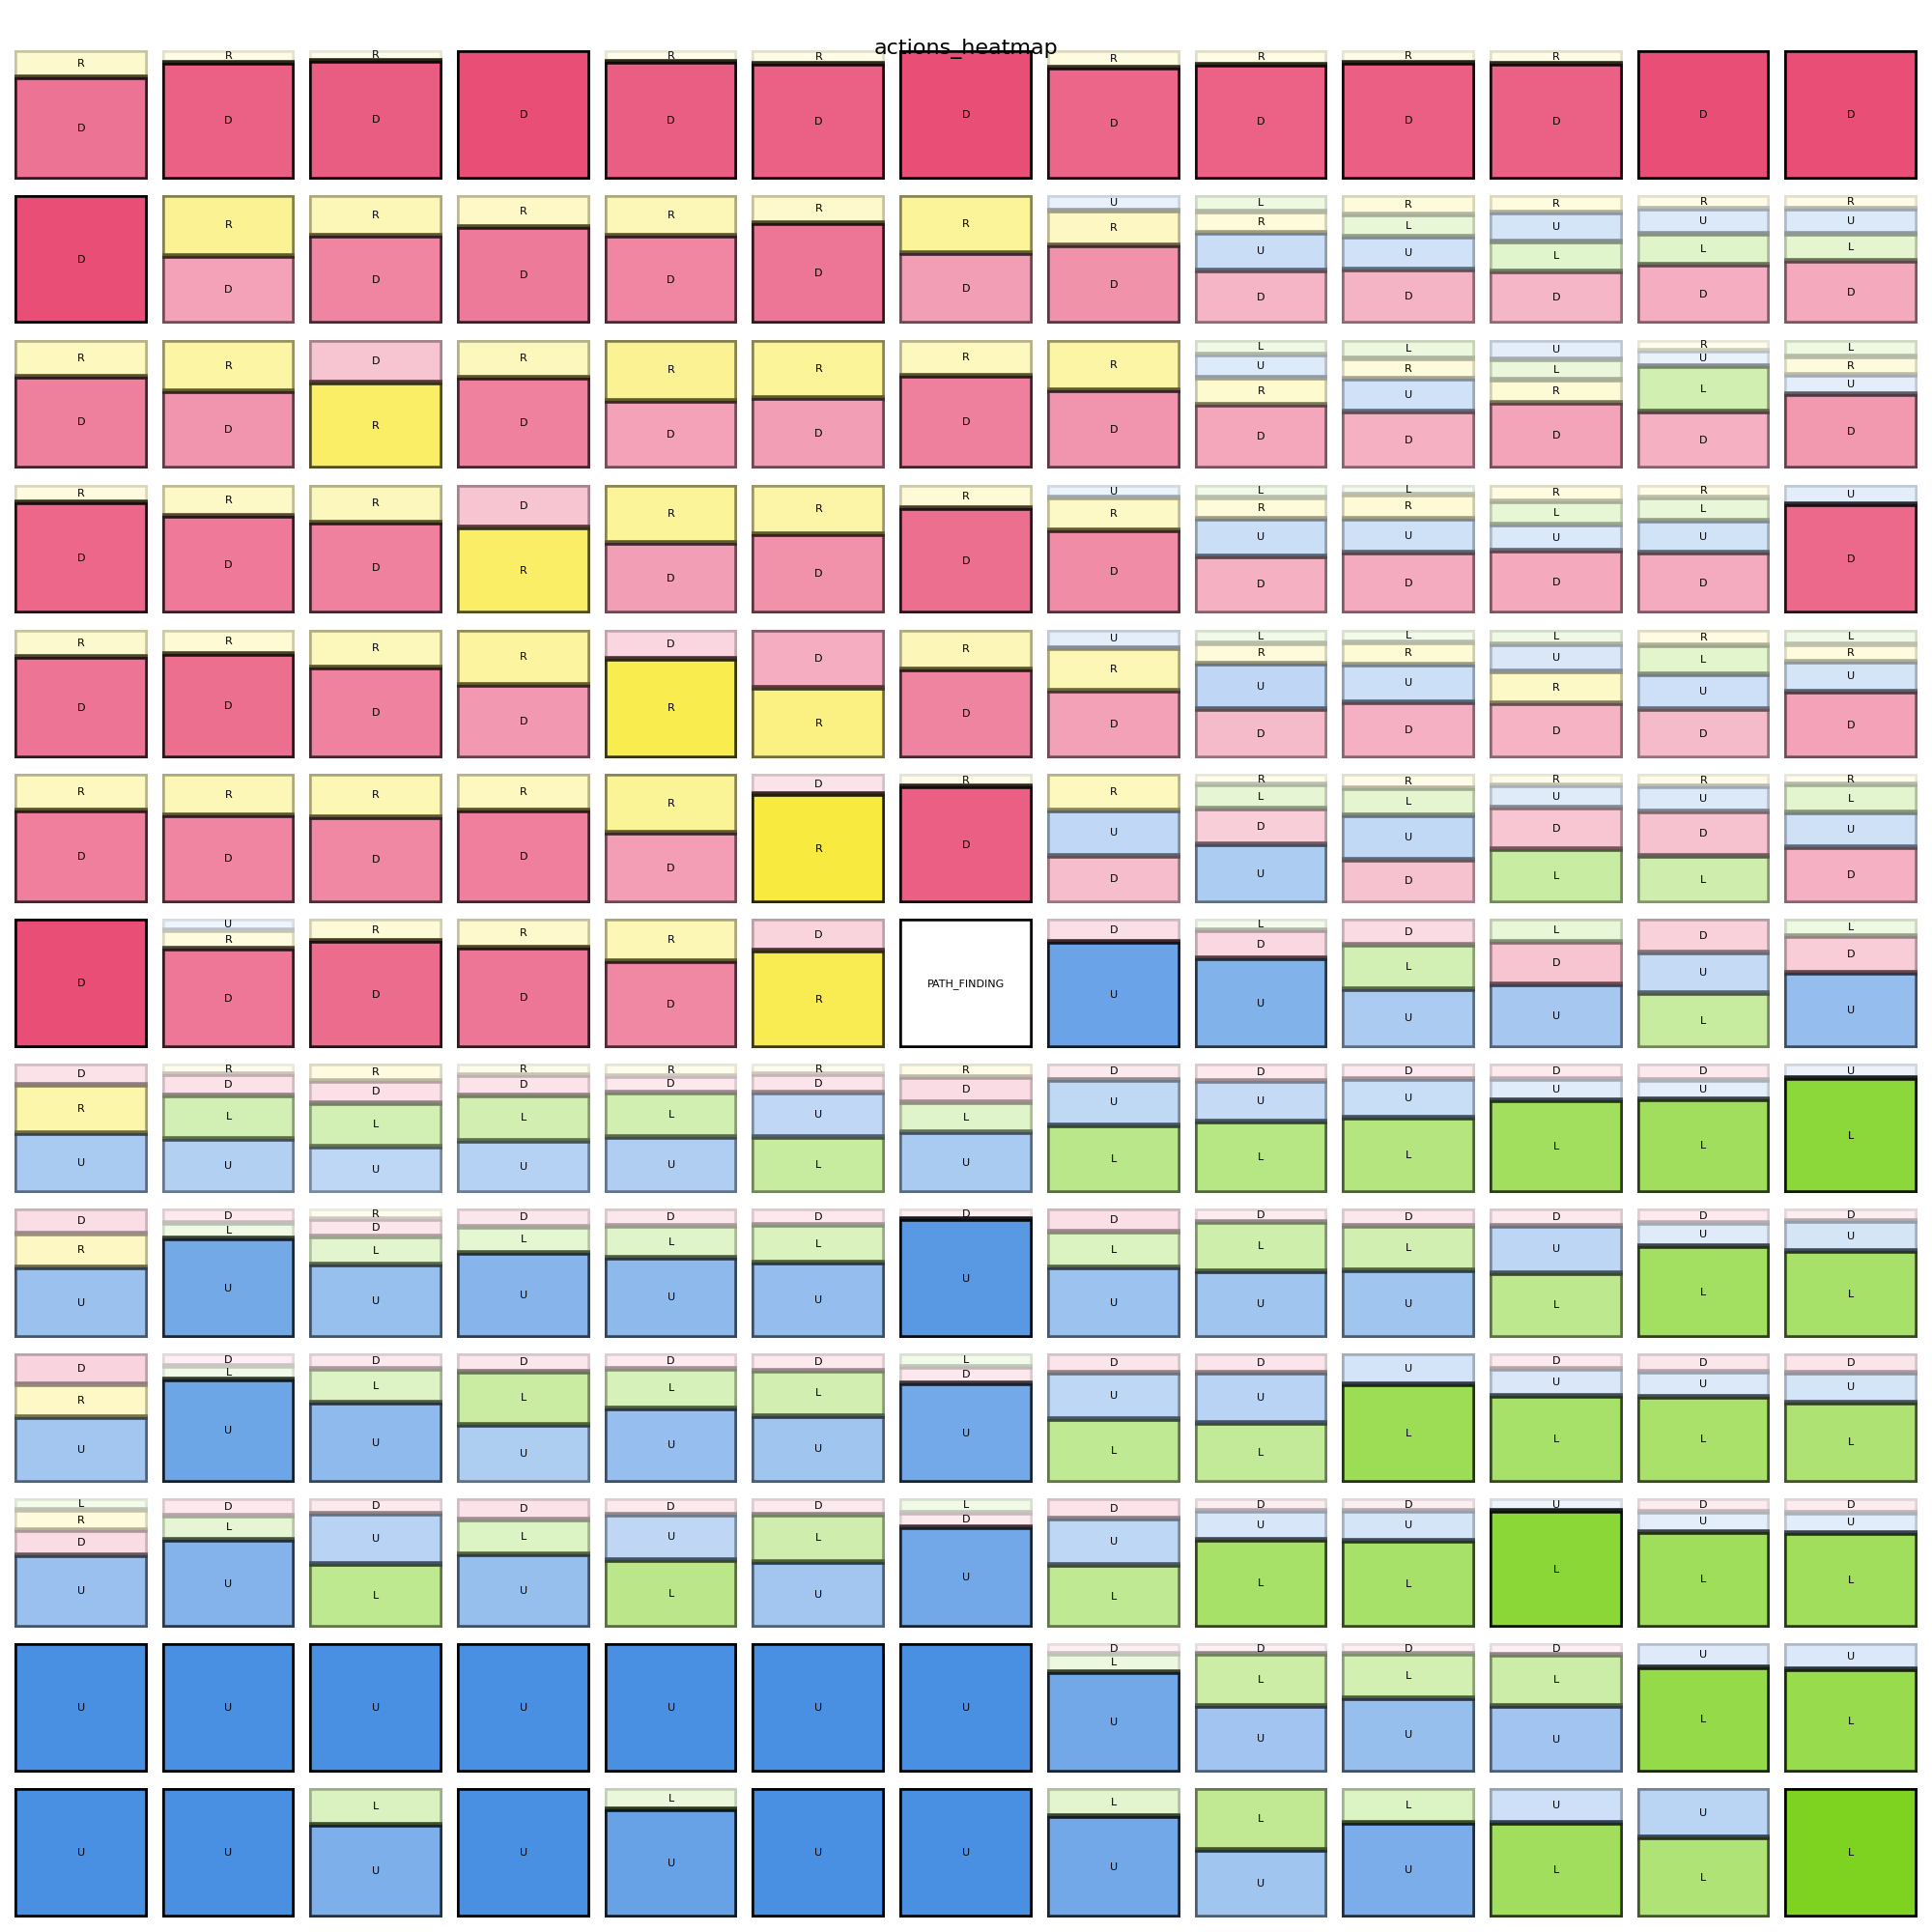
\includegraphics[width=\textwidth]{
      images/results_discussion/actions_heatmapTL.png
    }
    \caption{Top Left Orientation}
    \label{fig:heatmapTL}
  \end{minipage}
  \caption{Heatmaps showing actions with different map orientations}
  \label{fig:orientation}
\end{figure}

To further analyze the effect of orientation, we examined the correctness heatmaps
for both configurations, as shown in Figure \ref{fig:orientation_correctness}. The
results reveal a clear bias toward the top-left origin orientation, which we
refer to as the "programming origin," in contrast to the "Cartesian origin" commonly
used in mathematical contexts.

This bias may stem from the way the map was presented to the model. In our
specific implementation, the map was formatted as a list of tiles extracted from
a minimally edited JSON file. Given that JSON and other common data structures
in computer science often follow a top-left origin convention, it is likely that
the LLM was implicitly influenced by its prior knowledge from programming-related
contexts.

\vspace{5mm}
\begin{figure}[h]
  \centering
  \begin{minipage}[b]{0.45\textwidth}
    \centering
    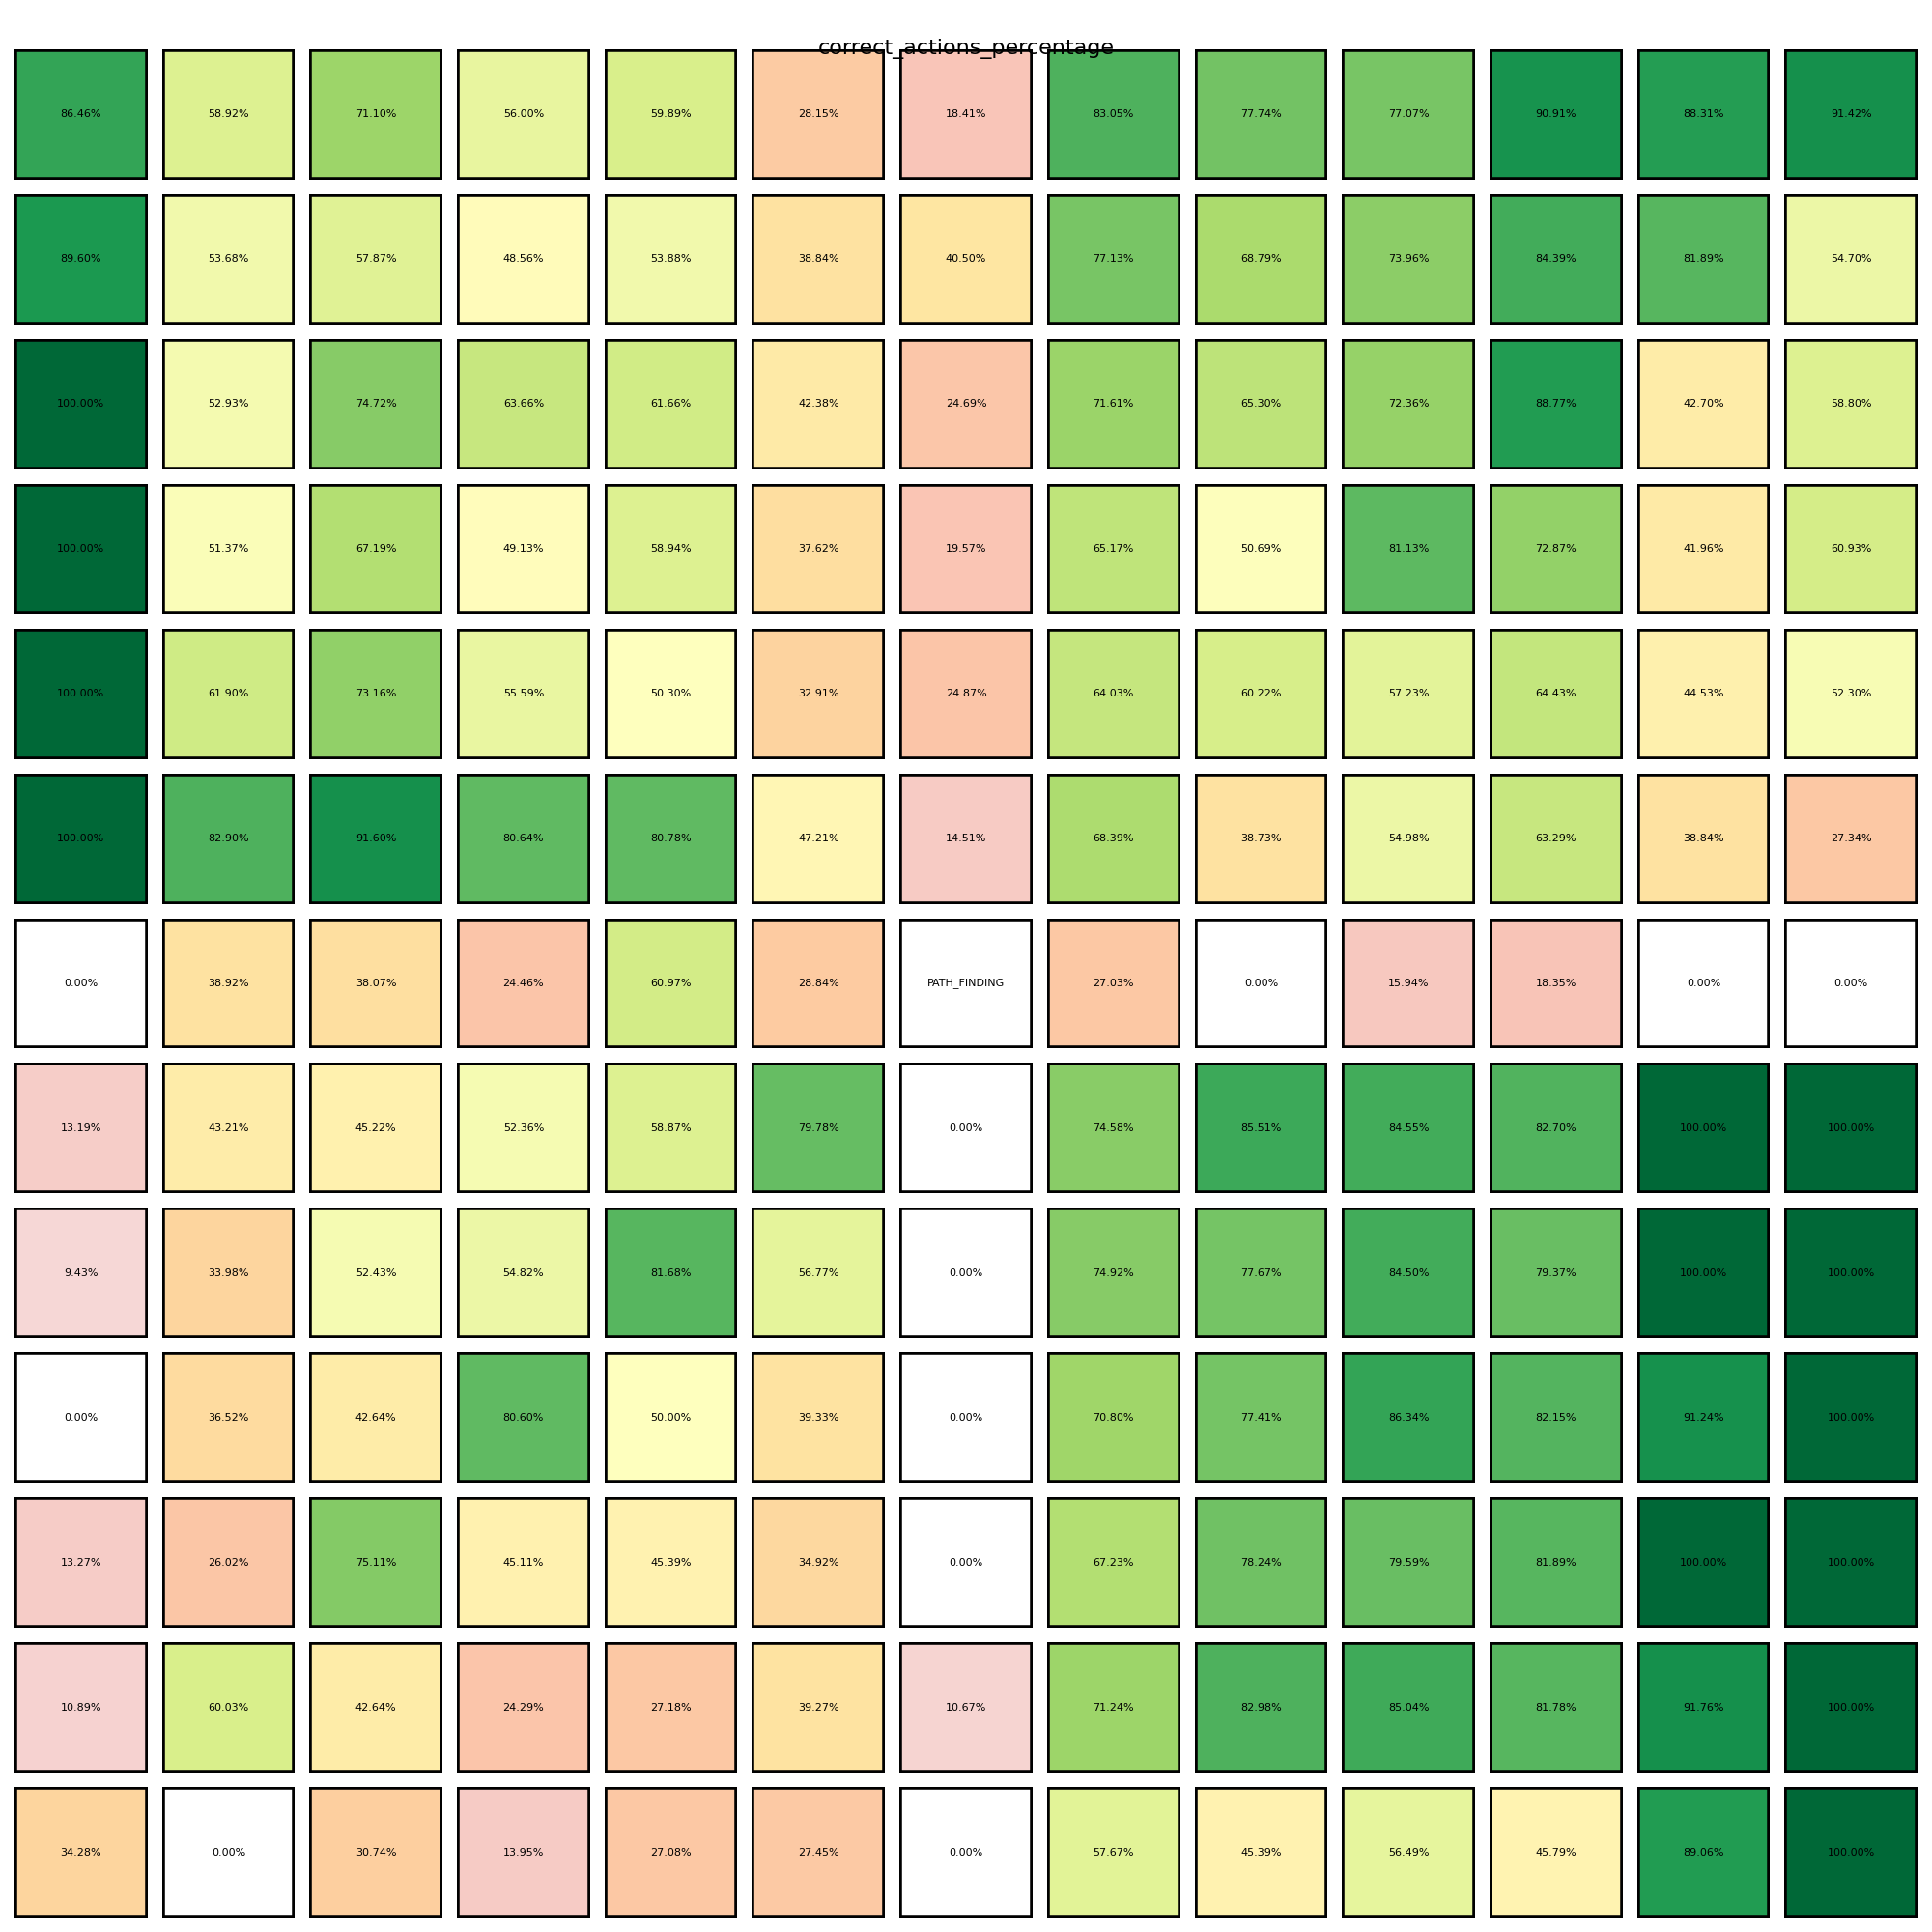
\includegraphics[width=\textwidth]{
      images/results_discussion/correctness_hm_BL.png
    }
    \caption{Bottom Left Orientation}
    \label{fig:heatmapBL}
  \end{minipage}
  \hfill
  \begin{minipage}[b]{0.45\textwidth}
    \centering
    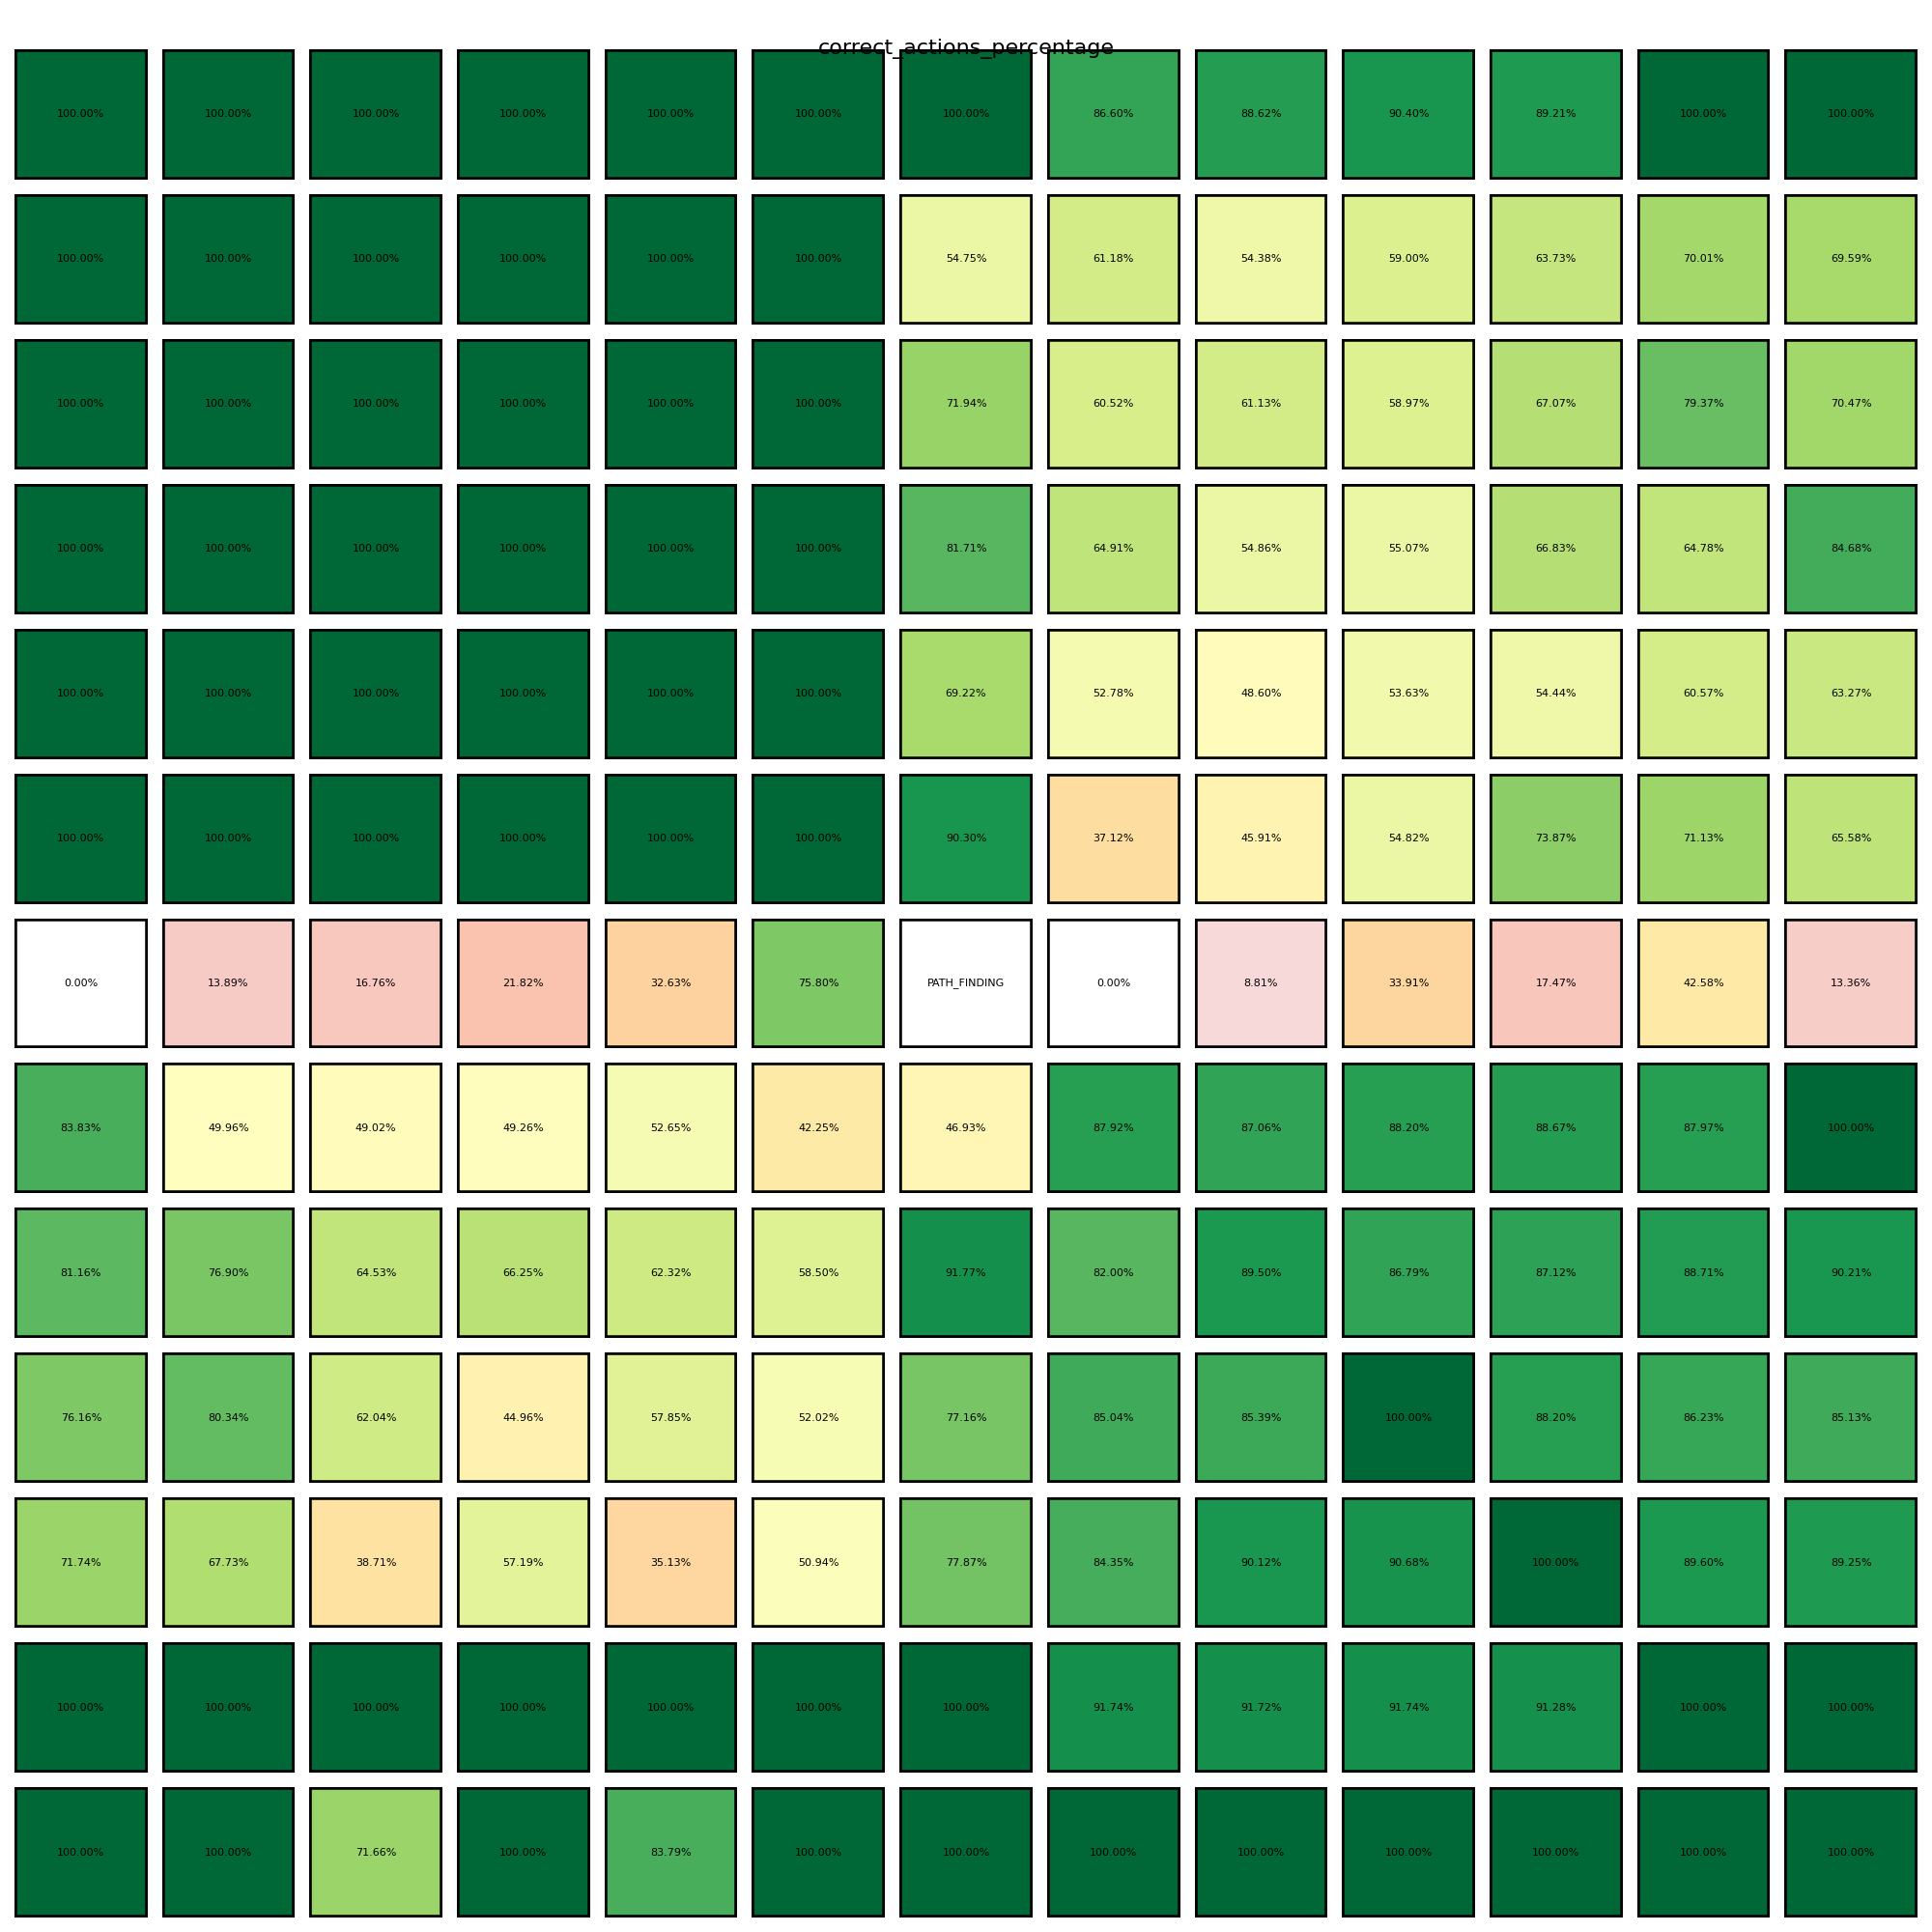
\includegraphics[width=\textwidth]{
      images/results_discussion/correctness_hm_TL.png
    }
    \caption{Top Left Orientation}
    \label{fig:heatmapTL}
  \end{minipage}
  \caption{Heatmaps showing correctness with different map orientations}
  \label{fig:orientation_correctness}
\end{figure}
\vspace{5mm}

\subsection{Comparison of Orientations}

When comparing the two orientations, we found that in the top-left origin
version, 154 tiles had one of the correct actions as the most probable choice.
In contrast, in the bottom-left origin version, only 104 tiles had a correct
action as the highest-probability choice. The comparison between the two orientations
reveals a clear preference for the top-left origin. The model performed
significantly better when using this orientation, as shown by the following accuracy
metrics:
\begin{itemize}
  \item \textbf{Top-left origin}: 92\% of the tiles had the correct action as
    the most probable one;

  \item \textbf{Bottom-left origin}: 62\% of the tiles had the correct action as
    the most probable one;

  \item \textbf{Top 3 actions comparison}: 99\% vs. 93\% of the tiles contained
    the correct action within the top three choices.
\end{itemize}

These results strongly suggest that the model is inherently biased toward the top-left
origin orientation. This finding highlights the potential influence of data
structure representations on LLM-based decision-making and suggests that models
trained on structured data formats may develop spatial preferences that impact
their performance in spatial reasoning tasks.

\section{Stateless}
\label{sec:stateless}

As previously discussed in Section \ref{sec:stateful_and_stateless_agents_chapAD},
a stateless agent operates without any memory of past actions or previous states
of the environment. In this context, every decision is made independently, relying
solely on the information provided within a single prompt.

Technically, each call to the Large Language Model (LLM) contains only the
current state of the environment, without any reference to past states or prior actions.
For every decision, a new conversation instance is initiated, making the agent
unable to build an internal representation of the map or track past movements.

One of the major challenges faced by a stateless agent is the need to infer its
position and the map layout solely based on the current prompt. This limitation leads
to several difficulties, such as:
\begin{itemize}
  \item \textbf{Inability to Track Progress:} Since the agent does not retain
    memory, it cannot recognize previously visited locations, often resulting in
    repetitive movements or getting stuck in loops.

  \item \textbf{Increased Uncertainty:} The LLM must deduce the correct course
    of action based only on the available snapshot of the environment, leading to
    occasional misinterpretations.

  \item \textbf{Higher Error Rates:} Compared to a stateful approach, where an agent
    can accumulate knowledge over time, the stateless method is more prone to
    making incorrect decisions, especially in larger maps.
\end{itemize}

Despite these challenges, implementing a stateless agent serves as an important step
toward understanding the inherent uncertainty in LLM-based decision-making. The
results obtained from this approach provide a useful baseline for evaluating the
potential benefits of incorporating statefulness.

The stateless agent follows predefined prompt templates, as described in Sections
\ref{sub:pickup_prompt} and \ref{sub:deliver_prompt}. These prompts encapsulate
all the necessary information about the current state and available actions
within a single request.

To evaluate the performance of the stateless agent, we analyze heatmaps generated
from experiments on different map sizes. The following sections present the
results for various scenarios.

\subsection{Pickup Goal at the Center}
\label{sub:pickup_goal_at_the_center}

Figures \ref{fig:stateless_pickup_heatmaps} and \ref{fig:stateless_pickup_correctness}
illustrate the heatmaps for maps of sizes 5x5, 7x7, and 13x13, with the pickup
goal placed at the center.

\vspace{5mm}
\begin{figure}[h]
  \centering
  \begin{minipage}[b]{0.32\textwidth}
    \centering
    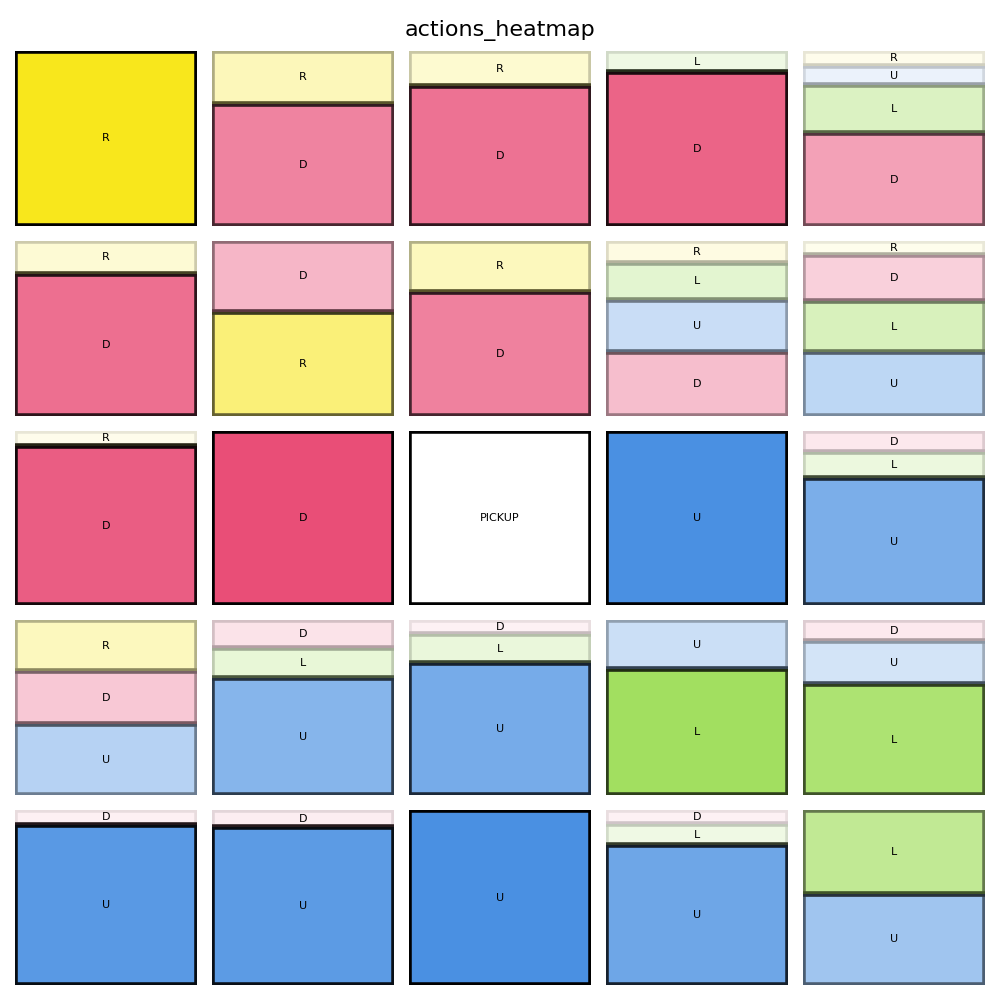
\includegraphics[width=\textwidth]{
      images/results_discussion/stateless/hm_5x5_pickup.png
    }
    \caption{5x5}
    \label{fig:hm_5x5_pickup}
  \end{minipage}
  \hfill
  \begin{minipage}[b]{0.32\textwidth}
    \centering
    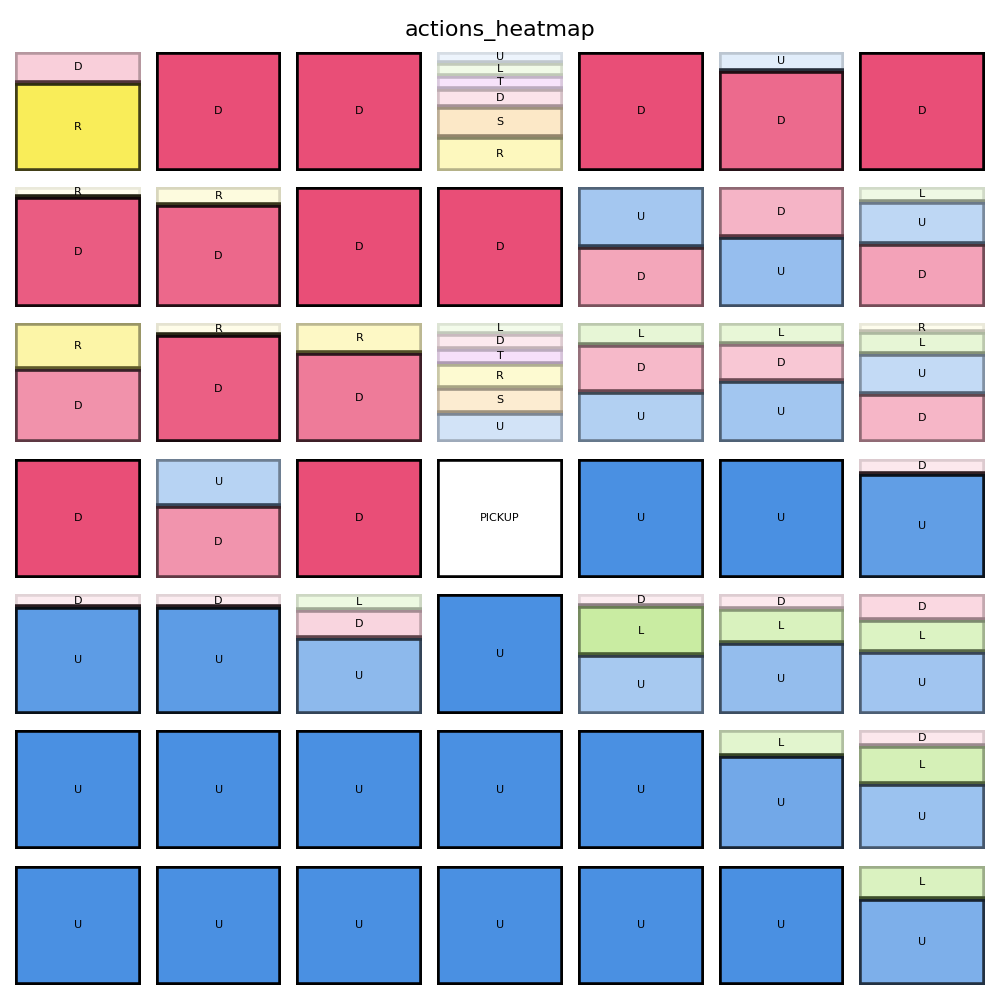
\includegraphics[width=\textwidth]{
      images/results_discussion/stateless/hm_7x7_pickup.png
    }
    \caption{7x7}
    \label{fig:hm_7x7_pickup}
  \end{minipage}
  \hfill
  \begin{minipage}[b]{0.32\textwidth}
    \centering
    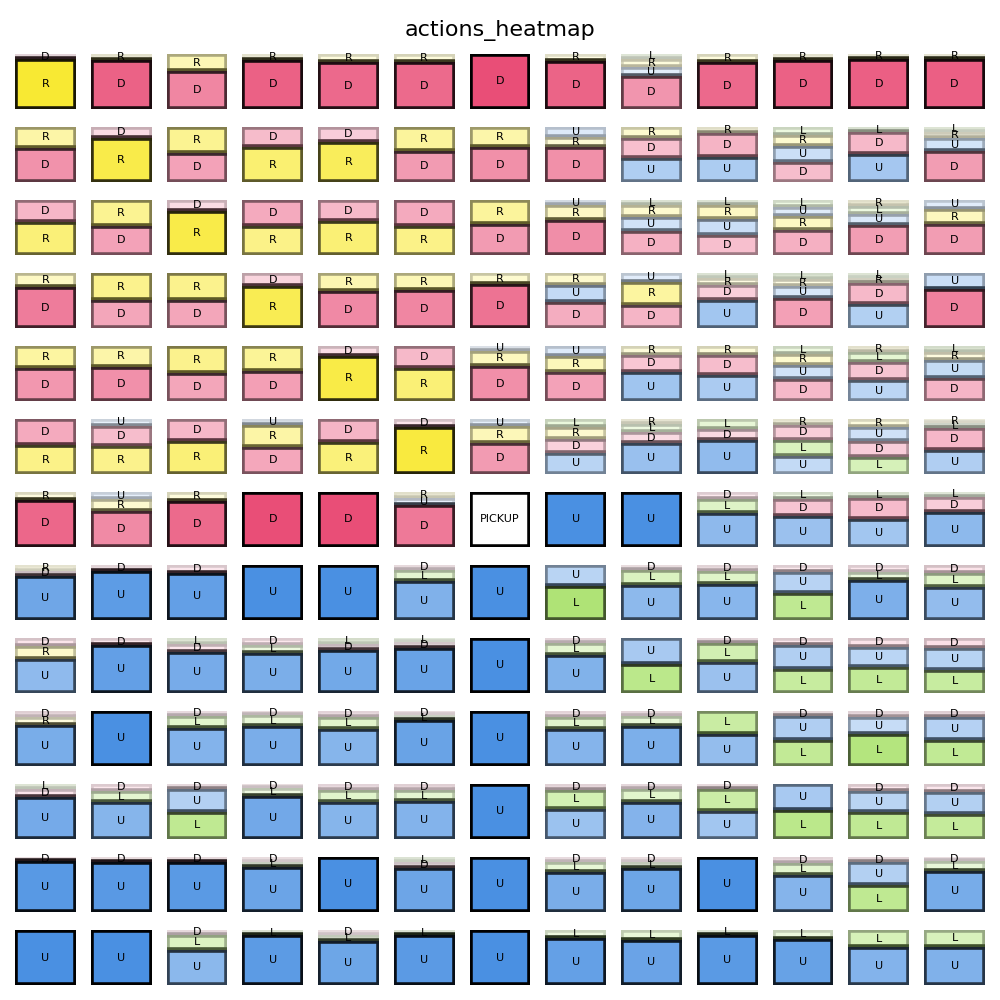
\includegraphics[width=\textwidth]{
      images/results_discussion/stateless/hm_13x13_pickup.png
    }
    \caption{13x13}
    \label{fig:hm_13x13_pickup}
  \end{minipage}
  \caption{Heatmaps for stateless agent with pickup goal in the center of
  different map sizes}
  \label{fig:stateless_pickup_heatmaps}
\end{figure}
\vspace{5mm}

From the heatmaps, we can observe a consistent pattern across different map
sizes. The top-left quadrant tends to show red and yellow as prominent colors and
the bottom-left quadrant is predominantly blue. The top-right quadrant exhibits
significant uncertainty with many actions in most of the cells, while the bottom-right
quadrant generally is green and blue (colors representing every actions, as explained
in Section \ref{sub:heatmaps}).

To further examine the correctness of the agent's decisions, we analyze the correctness
heatmaps shown in Figure \ref{fig:stateless_pickup_correctness}.

\vspace{5mm}
\begin{figure}[h]
  \centering
  \begin{minipage}[b]{0.32\textwidth}
    \centering
    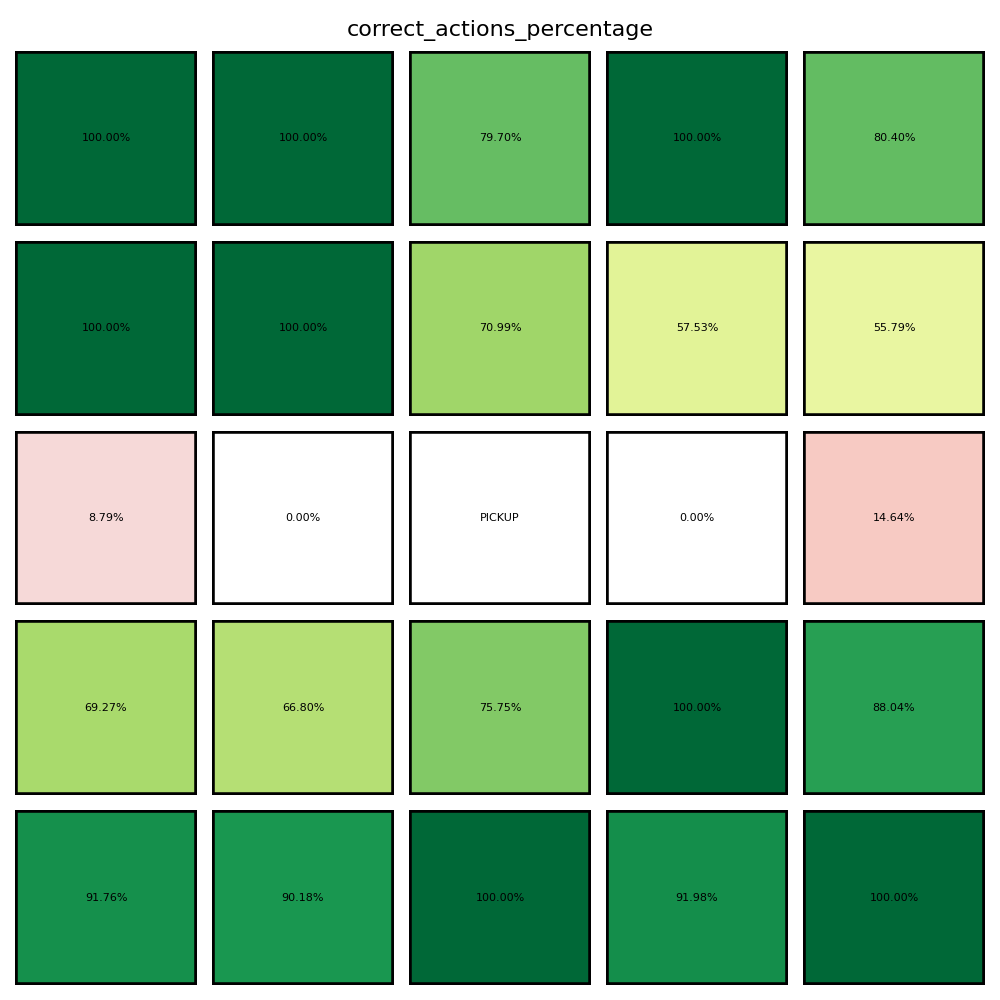
\includegraphics[width=\textwidth]{
      images/results_discussion/stateless/chm_5x5_pickup.png
    }
    \caption{5x5}
    \label{fig:chm_5x5_pickup}
  \end{minipage}
  \hfill
  \begin{minipage}[b]{0.32\textwidth}
    \centering
    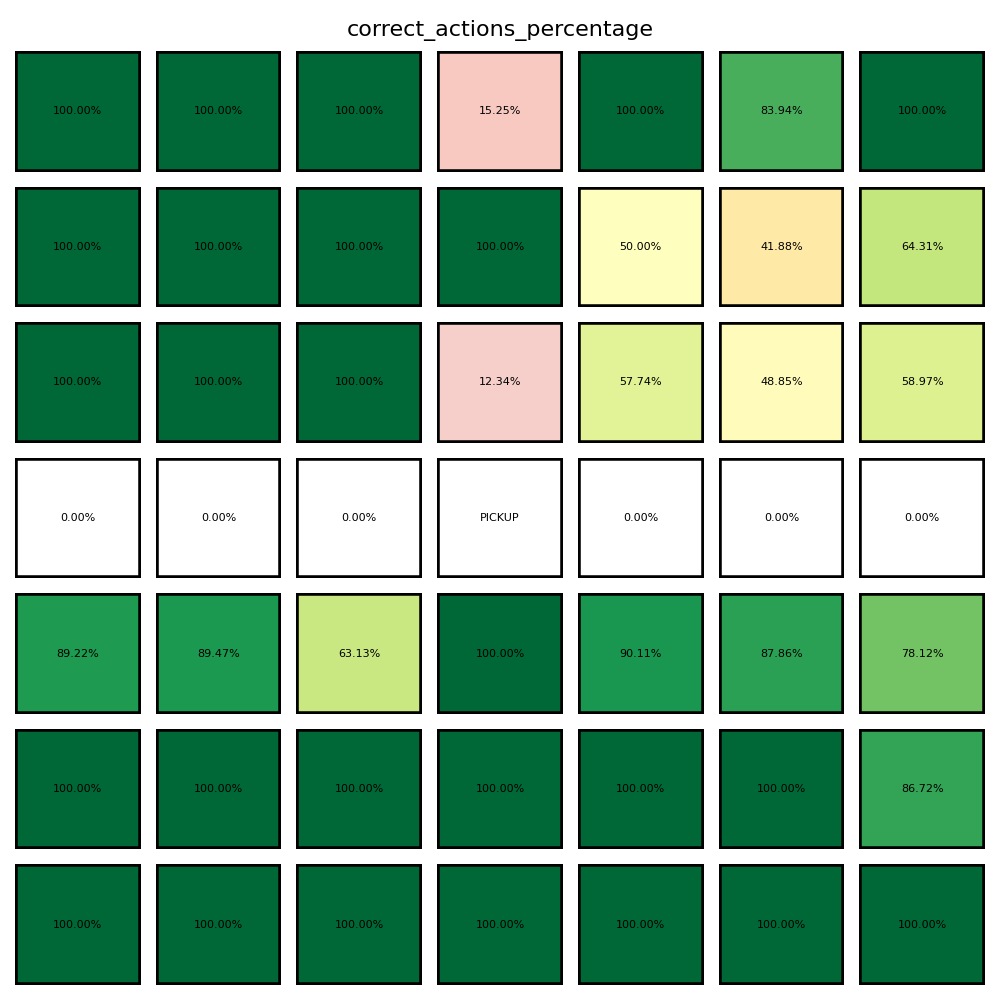
\includegraphics[width=\textwidth]{
      images/results_discussion/stateless/chm_7x7_pickup.png
    }
    \caption{7x7}
    \label{fig:chm_7x7_pickup}
  \end{minipage}
  \hfill
  \begin{minipage}[b]{0.32\textwidth}
    \centering
    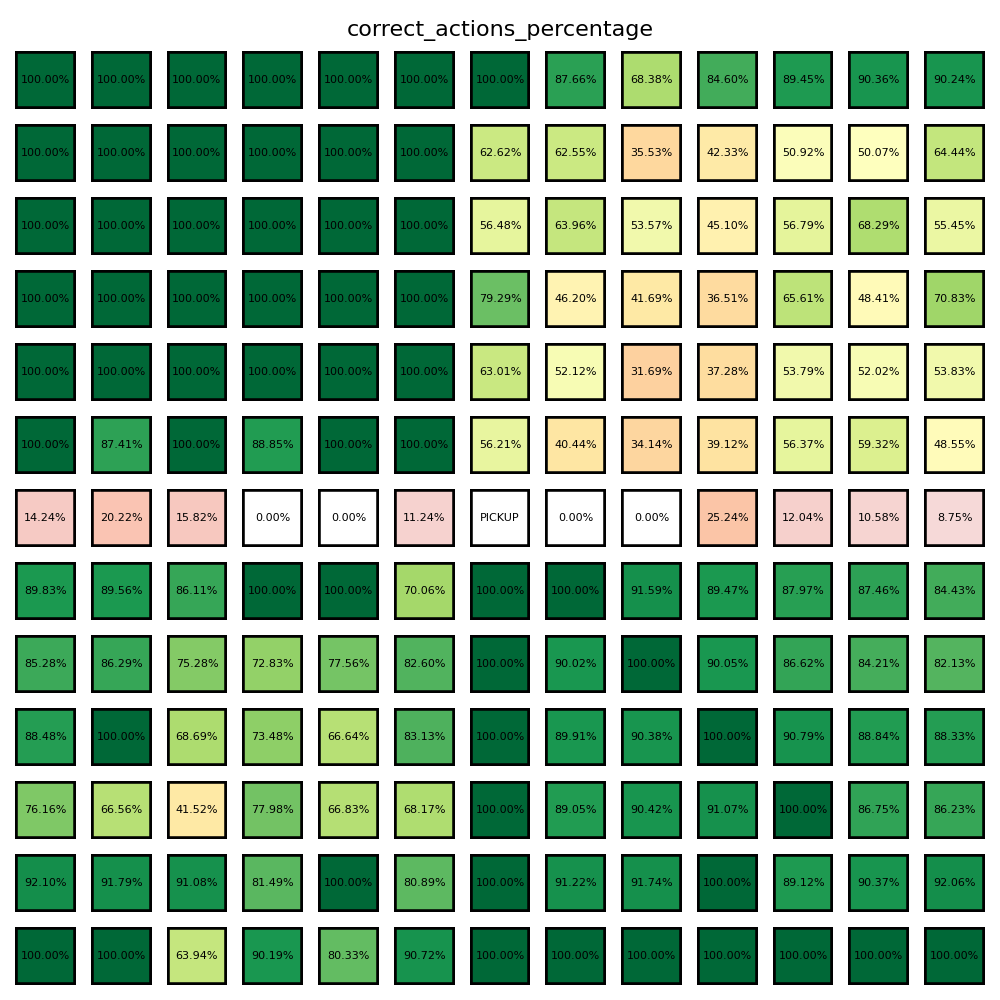
\includegraphics[width=\textwidth]{
      images/results_discussion/stateless/chm_13x13_pickup.png
    }
    \caption{13x13}
    \label{fig:chm_13x13_pickup}
  \end{minipage}
  \caption{Correctness heatmaps for stateless agent with pickup goal at the
  center of different map sizes.}
  \label{fig:stateless_pickup_correctness}
\end{figure}
\vspace{5mm}

The correctness analysis reveals the following trends:
\begin{itemize}
  \item The top-left and bottom-right quadrants exhibit the highest certainty,
    with the former being almost perfect in every cell;

  \item The top-right and bottom-left quadrants are more uncertain, with the top-right
    being the least reliable;

  \item Along the row and column containing the goal, the correctness tends to
    be lower, with several cells having 0\% correctness, meaning that the only correct
    action was discarded by KnowNo
\end{itemize}

Table \ref{tab:performance} presents numerical performance metrics across
different map sizes.

\vspace{5mm}
\begin{table}[h]
  \centering
  \begin{tabular}{c|ccc|ccc}
          & top1 & top2 & top3 & top1\% & top2\% & top3\% \\
    \hline
    5x5   & 19   & 22   & 22   & 0.792  & 0.917  & 0.917  \\
    7x7   & 37   & 40   & 41   & 0.771  & 0.833  & 0.854  \\
    13x13 & 125  & 161  & 162  & 0.744  & 0.958  & 0.964  \\
  \end{tabular}
  \caption{Performance metrics for different grid sizes}
  \label{tab:performance}
\end{table}
\vspace{5mm}

The results indicate that:
\begin{itemize}
  \item Smaller maps tend to yield a higher probability of selecting the correct
    action as the top-ranked choice.

  \item While absolute correctness decreases with increasing map size, the
    relative performance remains fairly stable.
\end{itemize}

Even if not visible in the heatmaps, the goal tile almost always had the correct
action as the only one kept after KnowNo framework, and rarely it kept other actions
but the correct one had a better probability by far. Only in one case, the ``goal
action" was the most probable also in the left cell wrt the goal.

\subsection{Deliver Goal at the Center}

A similar analysis can be conducted for the case where the delivery goal is placed
at the center of the map. Figures \ref{fig:stateless_deliver_heatmaps} and
\ref{fig:stateless_deliver_correctness} show the heatmaps for different map
sizes in this configuration.

Compared to the pickup task, the delivery task introduces slightly more uncertainty.
This uncertainty arises because, in our setup, the goal tile is not explicitly
marked as a destination in the prompt but must instead be inferred from the map
description. Again, the LLM needs to recognize that it has arrived at the
correct location based solely on relative positioning within the map, without any
persistent memory of past decisions.

From the heatmaps, we observe similar trends as seen in the pickup case:
\begin{itemize}
  \item The top-left and bottom-right quadrants show a higher concentration of correct
    probability;

  \item The top-right quadrant, similar to the pickup scenario, exhibits more variability
    and uncertainty;

  \item The row and column containing the goal continue to demonstrate reduced correctness.
\end{itemize}

\vspace{5mm}
\begin{figure}[h!]
  \centering
  \begin{minipage}[b]{0.32\textwidth}
    \centering
    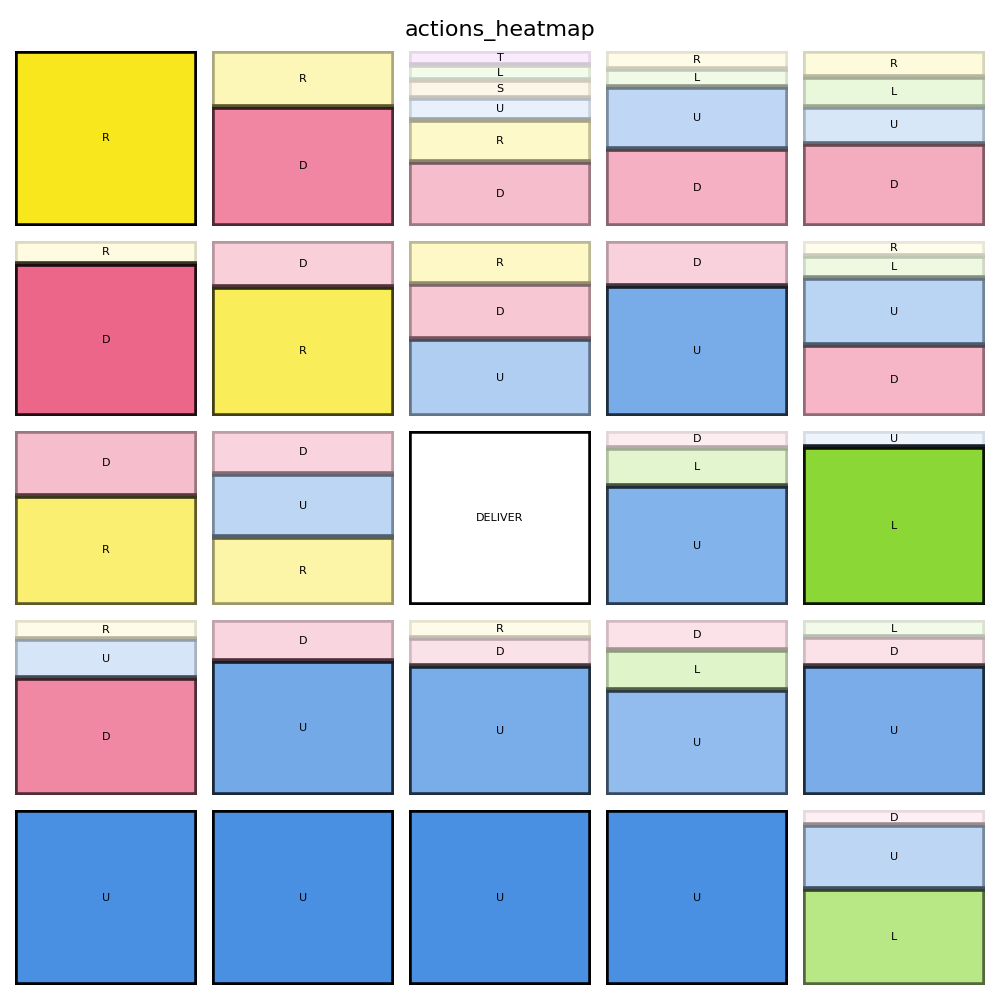
\includegraphics[width=\textwidth]{
      images/results_discussion/stateless/hm_5x5_deliver.png
    }
    \caption{5x5}
    \label{fig:hm_5x5_deliver}
  \end{minipage}
  \hfill
  \begin{minipage}[b]{0.32\textwidth}
    \centering
    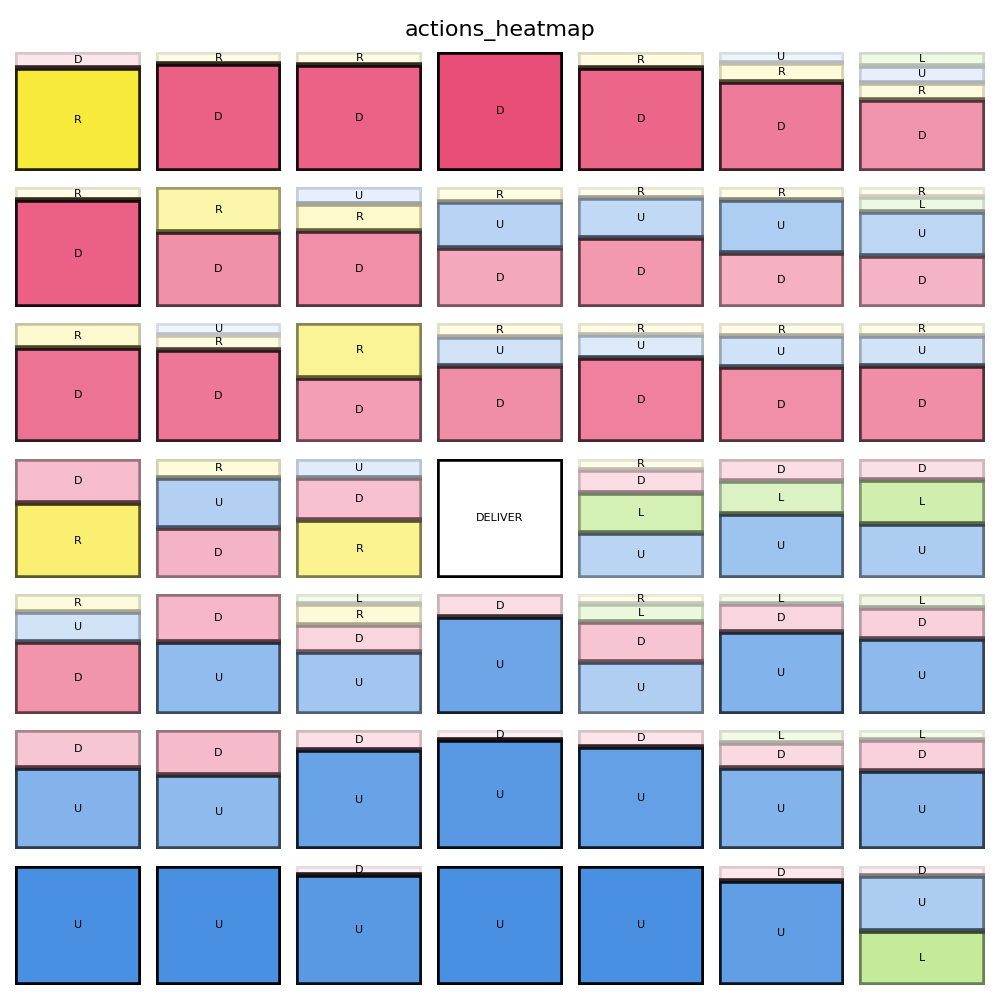
\includegraphics[width=\textwidth]{
      images/results_discussion/stateless/hm_7x7_deliver.png
    }
    \caption{7x7}
    \label{fig:hm_7x7_deliver}
  \end{minipage}
  \hfill
  \begin{minipage}[b]{0.32\textwidth}
    \centering
    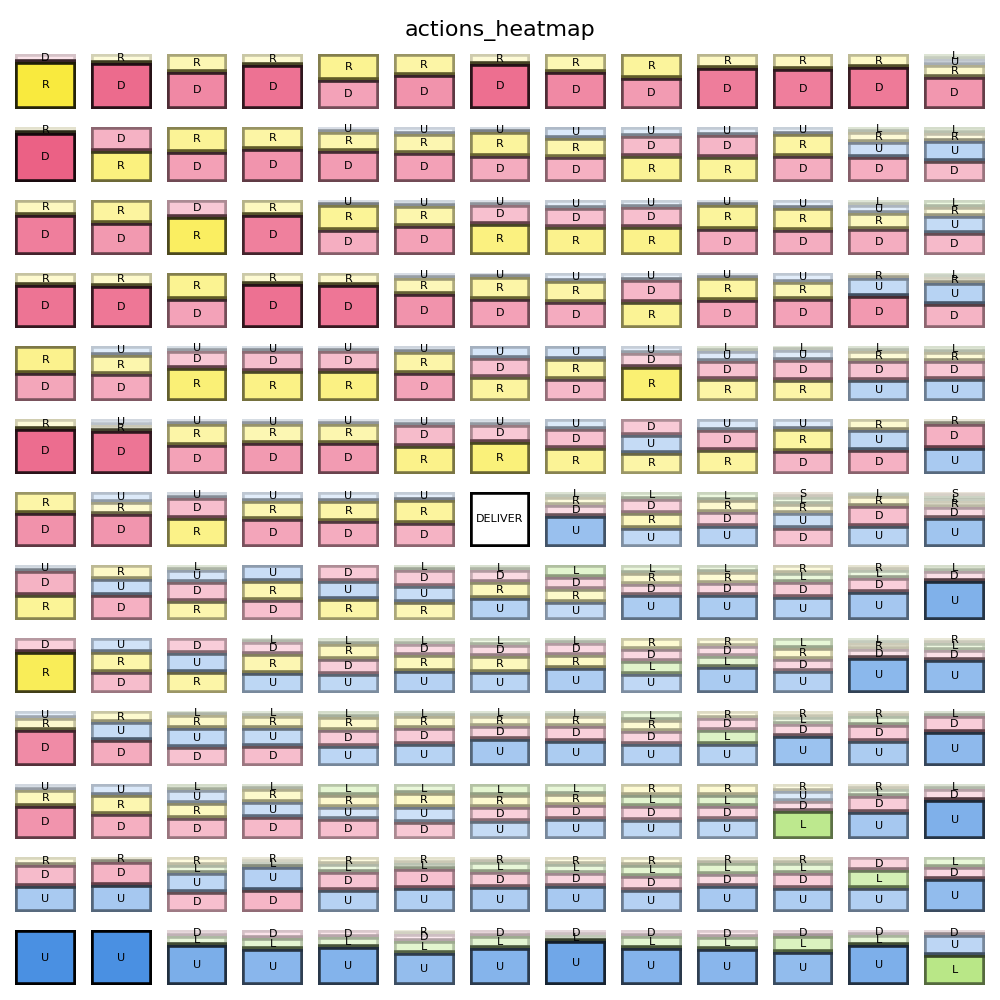
\includegraphics[width=\textwidth]{
      images/results_discussion/stateless/hm_13x13_deliver.png
    }
    \caption{13x13}
    \label{fig:hm_13x13_deliver}
  \end{minipage}
  \caption{Heatmaps for stateless agent with deliver goal in the center of
  different map sizes}
  \label{fig:stateless_deliver_heatmaps}
\end{figure}
\vspace{5mm}

\vspace{5mm}
\begin{figure}[h!]
  \centering
  \begin{minipage}[b]{0.32\textwidth}
    \centering
    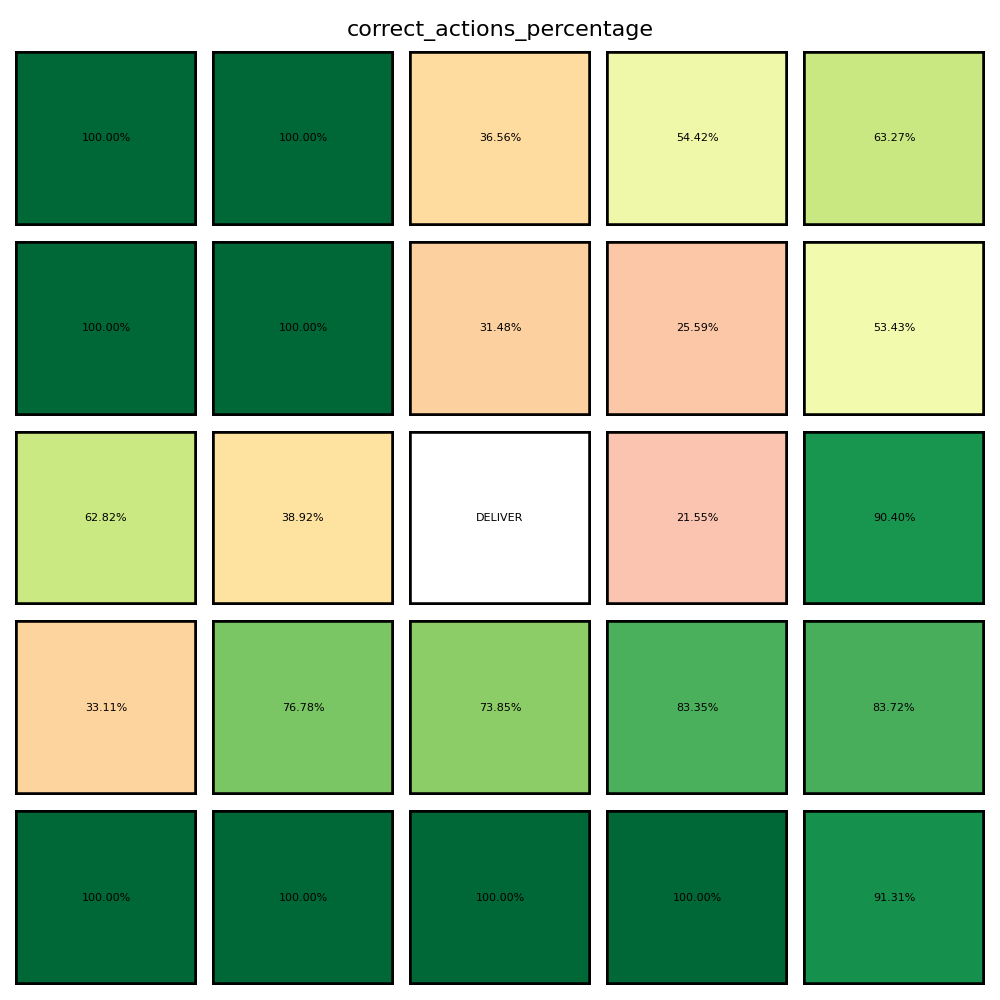
\includegraphics[width=\textwidth]{
      images/results_discussion/stateless/chm_5x5_deliver.png
    }
    \caption{5x5}
    \label{fig:chm_5x5_deliver}
  \end{minipage}
  \hfill
  \begin{minipage}[b]{0.32\textwidth}
    \centering
    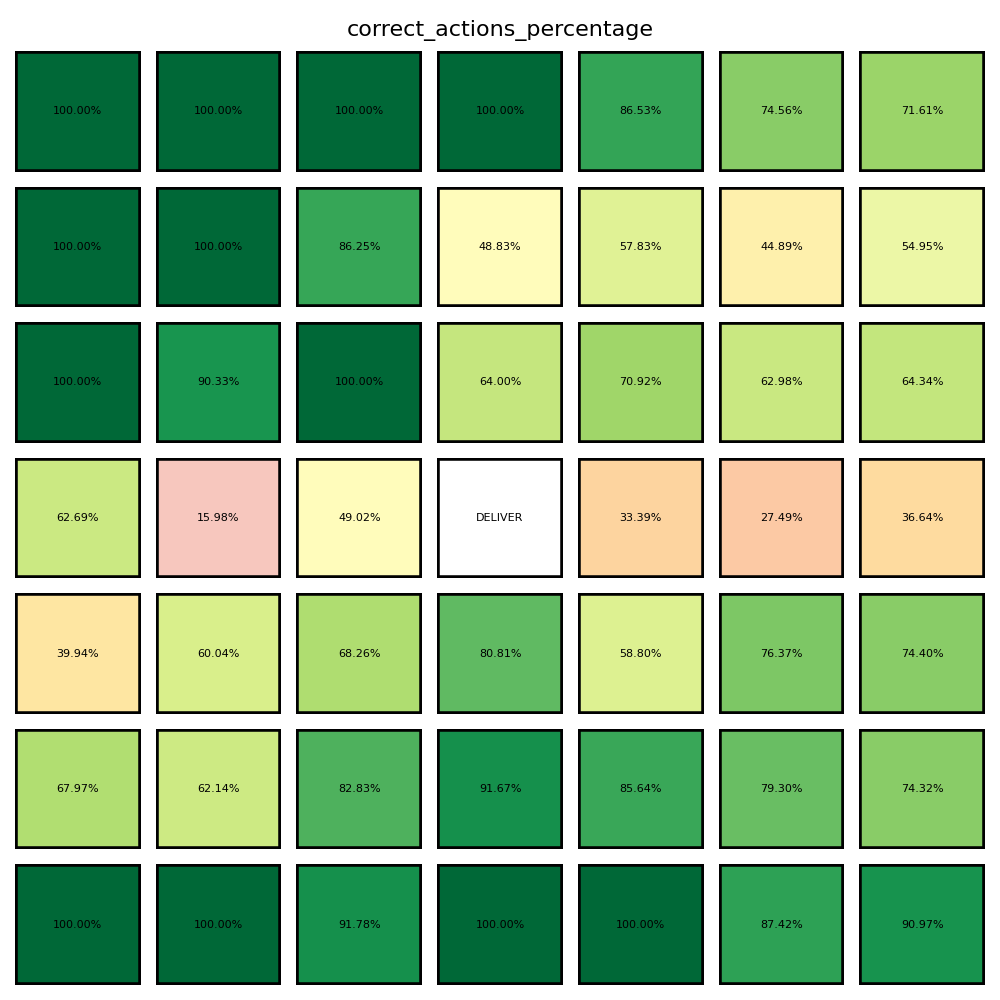
\includegraphics[width=\textwidth]{
      images/results_discussion/stateless/chm_7x7_deliver.png
    }
    \caption{7x7}
    \label{fig:chm_7x7_deliver}
  \end{minipage}
  \hfill
  \begin{minipage}[b]{0.32\textwidth}
    \centering
    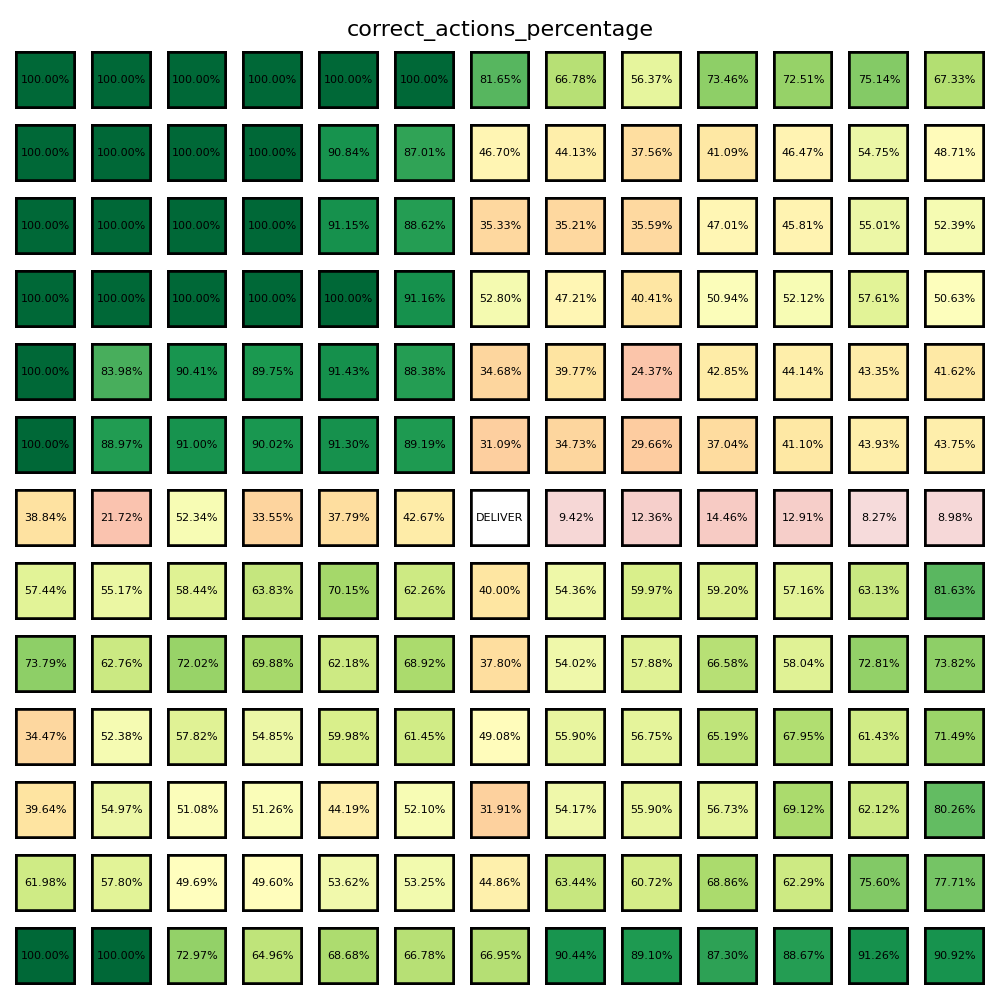
\includegraphics[width=\textwidth]{
      images/results_discussion/stateless/chm_13x13_deliver.png
    }
    \caption{13x13}
    \label{fig:chm_13x13_deliver}
  \end{minipage}
  \caption{Heatmaps for stateless agent with deliver goal in the center of
  different map sizes}
  \label{fig:stateless_deliver_correctness}
\end{figure}
\vspace{5mm}

Moreover, the values in Table \ref{tab:performance} reveals that as the map size
increases, the probability of selecting the correct action as the top-ranked
choice decreases. However, the overall trend remains consistent, suggesting that
while uncertainty increases with map size, the general patterns of decision-making
remain largely stable across different scales.

\vspace{5mm}
\begin{table}[h!]
  \centering
  \begin{tabular}{c|ccc|ccc}
          & top1 & top2 & top3 & top1\% & top2\% & top3\% \\
    \hline
    5x5   & 20   & 24   & 24   & 0.833  & 1.000  & 1.000  \\
    7x7   & 43   & 47   & 48   & 0.896  & 0.979  & 1.000  \\
    13x13 & 125  & 161  & 162  & 0.744  & 0.958  & 0.964  \\
  \end{tabular}
  \caption{Performance metrics for different grid sizes}
  \label{tab:performance}
\end{table}
\vspace{5mm}

\subsection{Pickup and Deliver Goals in Different Map Sections}

Beyond testing the performance of the stateless agent scenarios with the goal at
the center, we also examined its ability to handle pickup and delivery goals positioned
in different sections of the map. Figures \ref{fig:stateless_top_right} and
\ref{fig:stateless_bottom_right} illustrate the heatmaps for cases where the
pickup and delivery locations are in the top-right and bottom-right corners, respectively.

By analyzing the performance in these different regions, we aim to understand
whether the placement of the goal influences the decision-making accuracy of the
LLM. Since the map is embedded within a structured text prompt, the location of
the goal may impact how the LLM processes the spatial relationships between
different tiles as explained in Section \ref{sub:goal_positioning}.

\vspace{5mm}
\begin{figure}[h!]
  \centering
  \begin{minipage}[b]{0.45\textwidth}
    \centering
    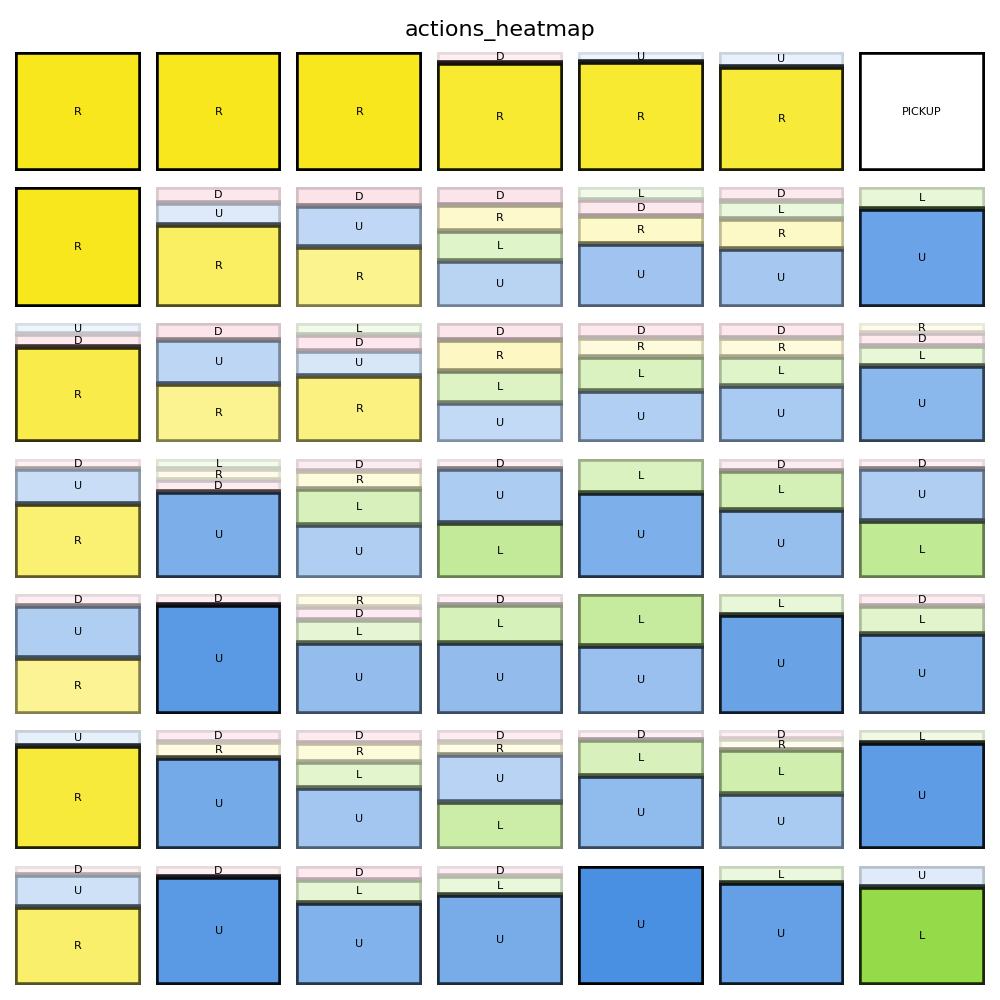
\includegraphics[width=\textwidth]{
      images/results_discussion/stateless/not_central/stateless_pickup_top_right.png
    }
    \caption{Pickup Top Right}
    \label{fig:stateless_pickup_top_right}
  \end{minipage}
  \hfill
  \begin{minipage}[b]{0.45\textwidth}
    \centering
    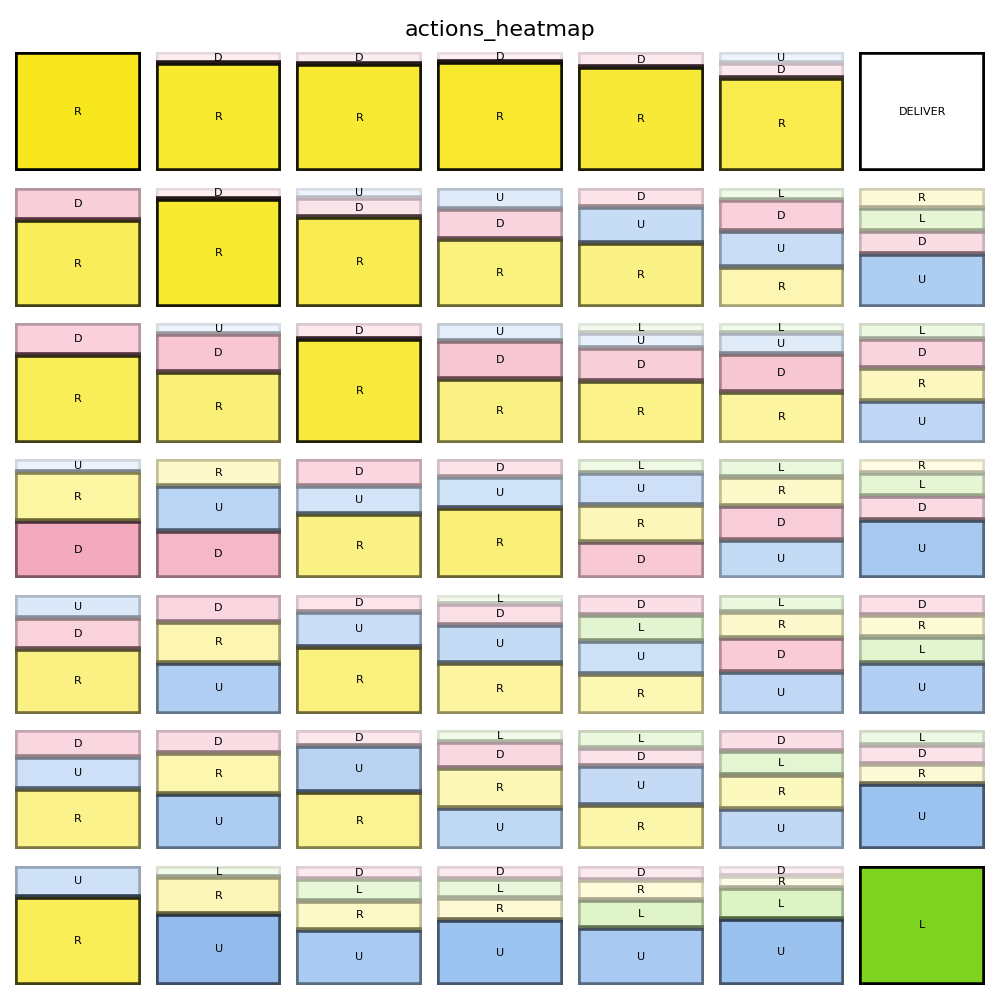
\includegraphics[width=\textwidth]{
      images/results_discussion/stateless/not_central/stateless_deliver_top_right.png
    }
    \caption{Deliver Top Right}
    \label{fig:stateless_deliver_top_right}
  \end{minipage}
  \caption{Heatmaps for stateless agent with pickup and deliver goals in the top
  right corner of the map}
  \label{fig:stateless_top_right}
\end{figure}
\vspace{5mm}

\begin{figure}[h!]
  \centering
  \begin{minipage}[b]{0.45\textwidth}
    \centering
    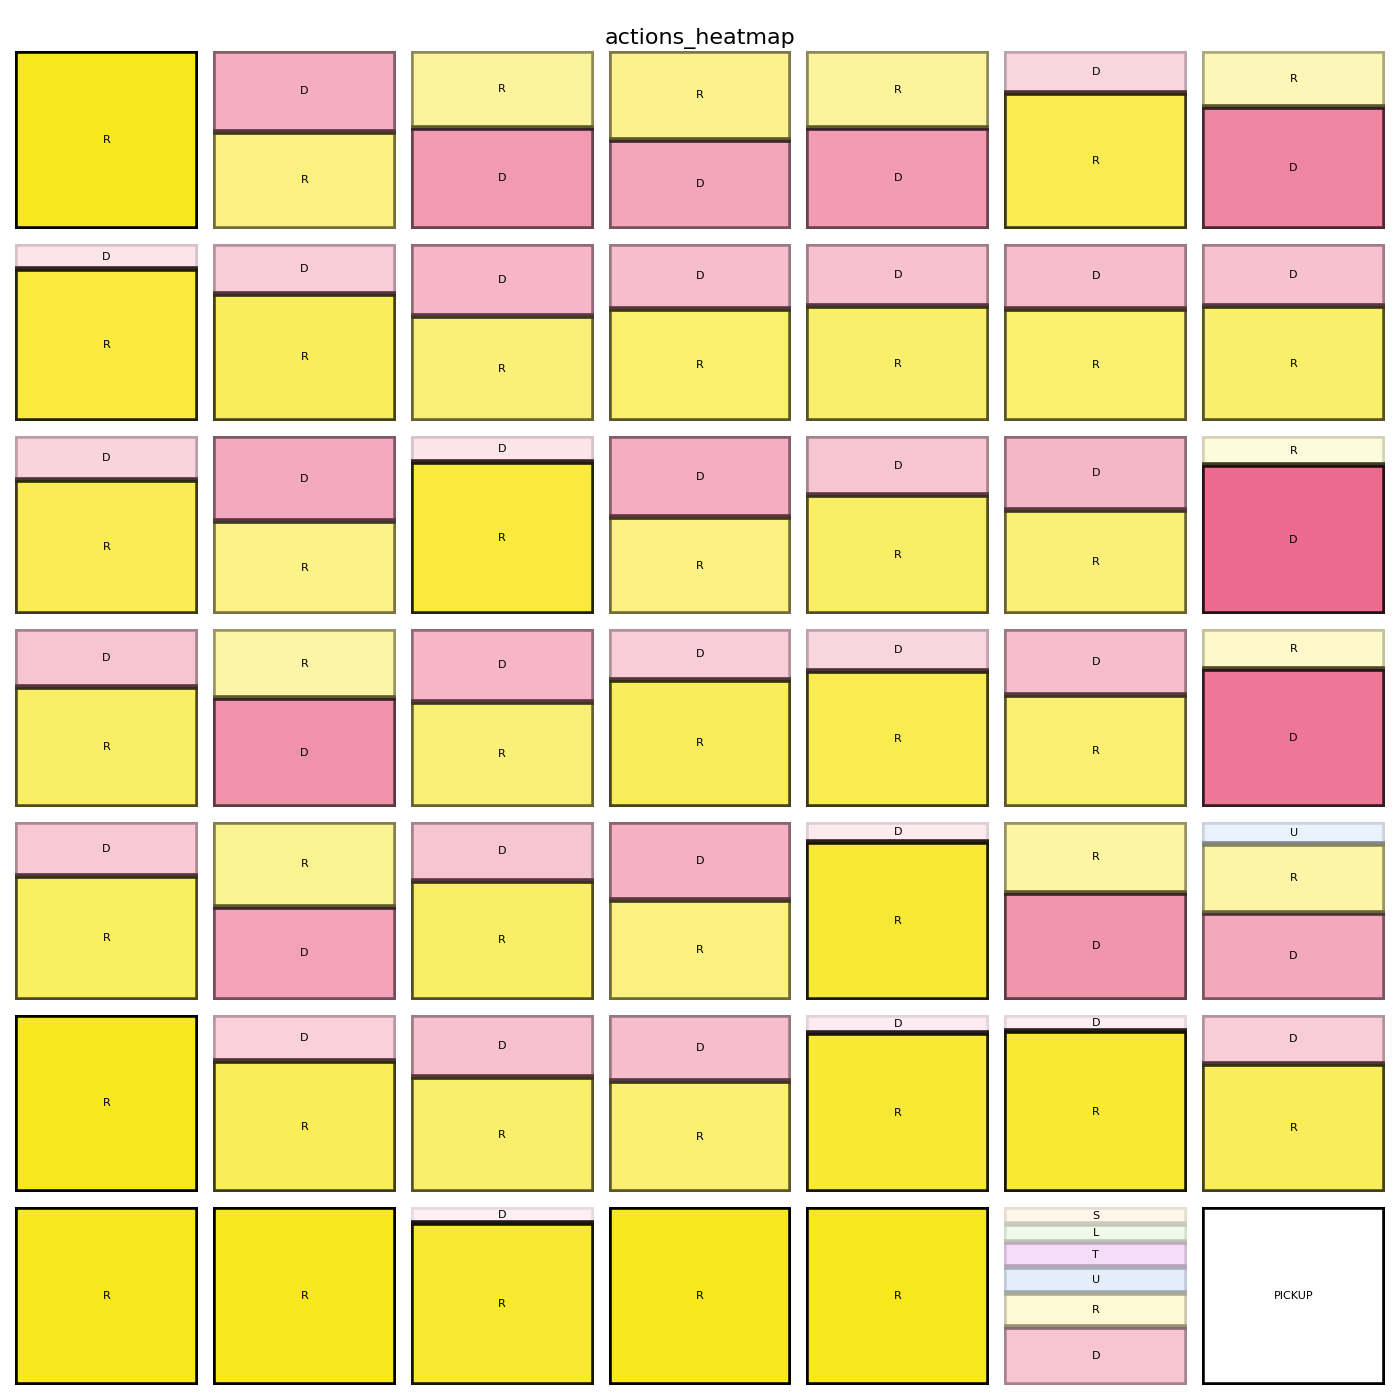
\includegraphics[width=\textwidth]{
      images/results_discussion/stateless/not_central/stateless_pickup_bottom_right.png
    }
    \caption{Pickup Bottom Right}
    \label{fig:stateless_pickup_bottom_right}
  \end{minipage}
  \hfill
  \begin{minipage}[b]{0.45\textwidth}
    \centering
    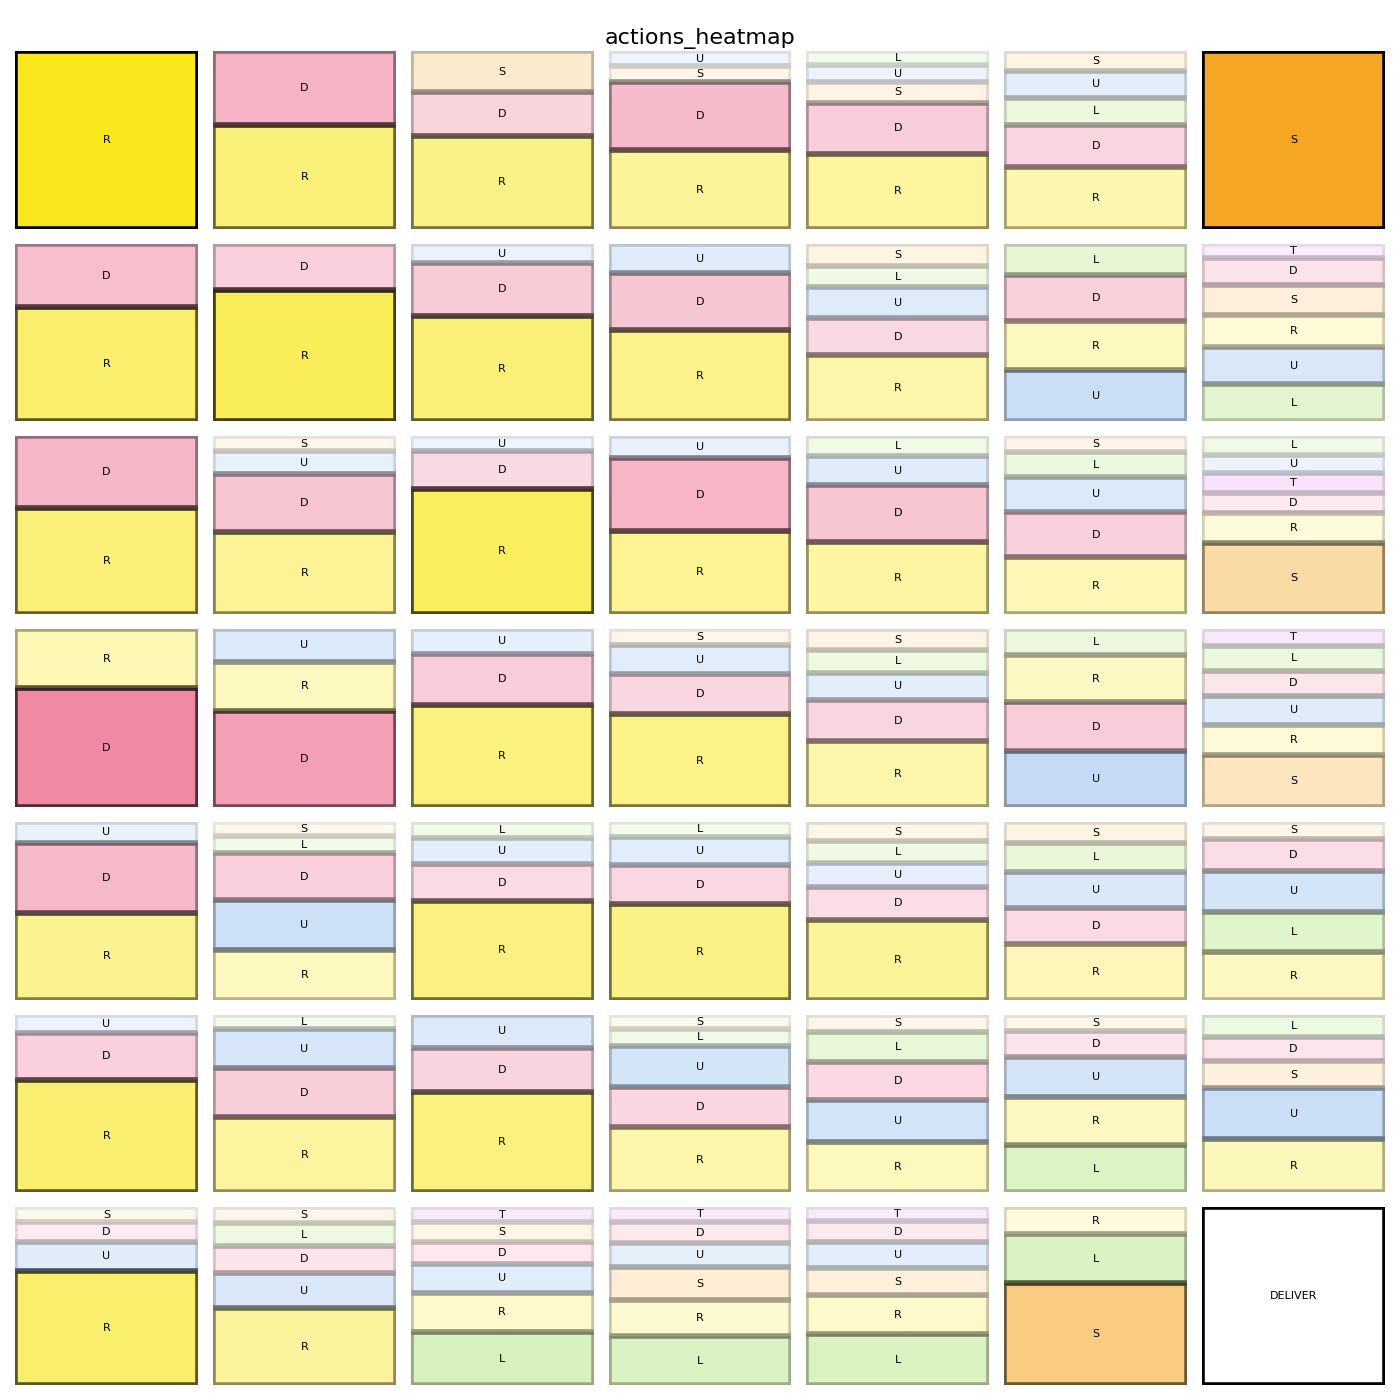
\includegraphics[width=\textwidth]{
      images/results_discussion/stateless/not_central/stateless_deliver_bottom_right.png
    }
    \caption{Deliver Bottom Right}
    \label{fig:stateless_deliver_bottom_right}
  \end{minipage}
  \caption{Heatmaps for stateless agent with pickup and deliver goals in the
  bottom right corner of the map}
  \label{fig:stateless_bottom_right}
\end{figure}
\vspace{5mm}

Looking at the correctness heatmaps in Figures
\ref{fig:stateless_top_right_correctness} and
\ref{fig:stateless_bottom_right_correctness}, we observe similar patterns, where
the characteristic drop in correctness along the goal row and column persists.

\vspace{5mm}
\begin{figure}[h]
  \centering
  \begin{minipage}[b]{0.45\textwidth}
    \centering
    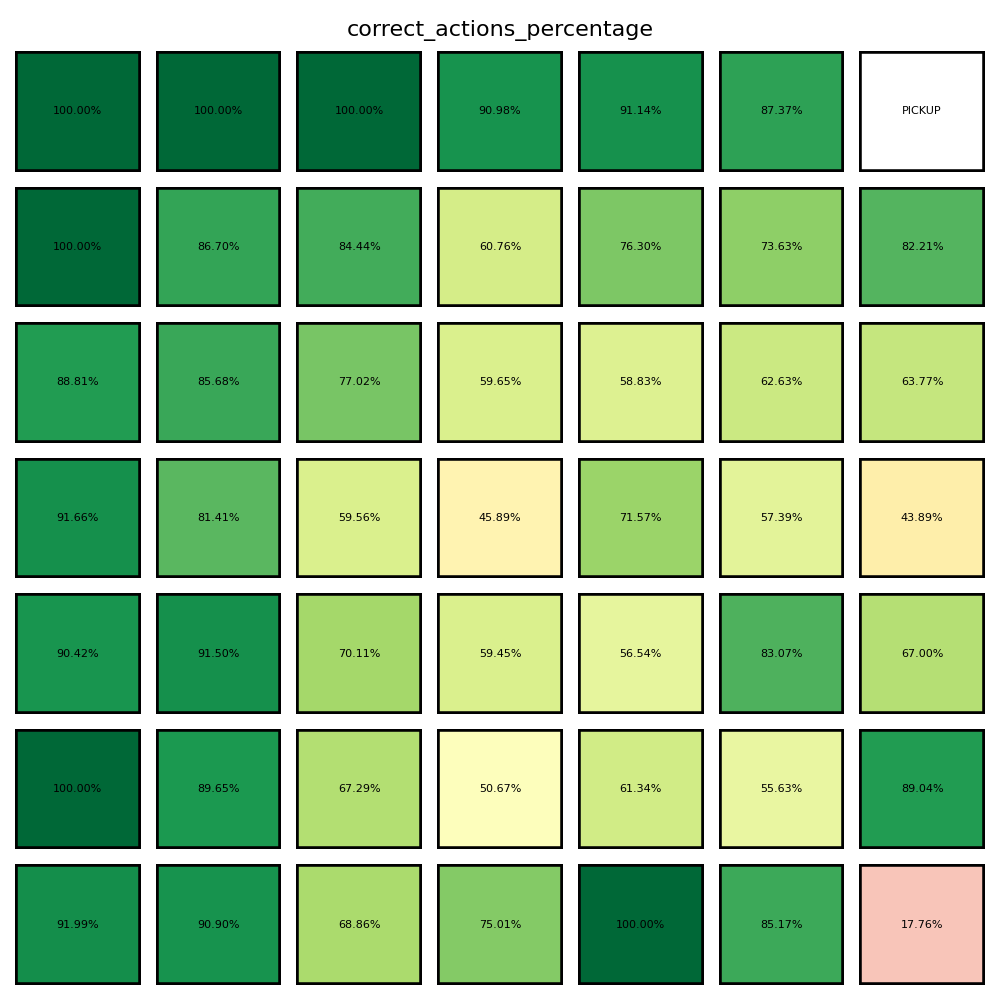
\includegraphics[width=\textwidth]{
      images/results_discussion/stateless/not_central/chm_pickup_top_right.png
    }
    \caption{Correctness Pickup Top Right}
    \label{fig:chm_pickup_top_right}
  \end{minipage}
  \hfill
  \begin{minipage}[b]{0.45\textwidth}
    \centering
    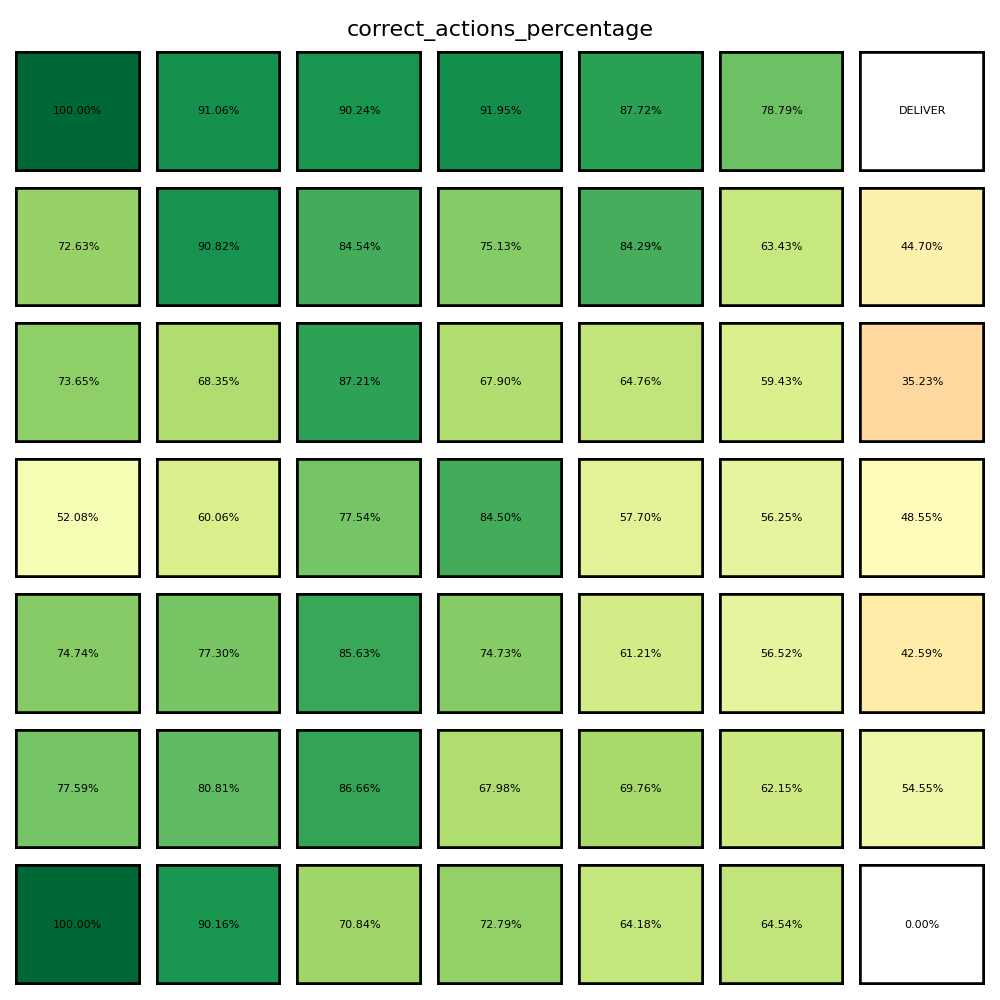
\includegraphics[width=\textwidth]{
      images/results_discussion/stateless/not_central/chm_deliver_top_right.png
    }
    \caption{Correctness Deliver Top Right}
    \label{fig:chm_deliver_top_right}
  \end{minipage}
  \caption{Correctness heatmaps for stateless agent with pickup and deliver
  goals in the top right corner of the map}
  \label{fig:stateless_top_right_correctness}
\end{figure}
\vspace{5mm}

\vspace{5mm}
\begin{figure}[h]
  \centering
  \begin{minipage}[b]{0.45\textwidth}
    \centering
    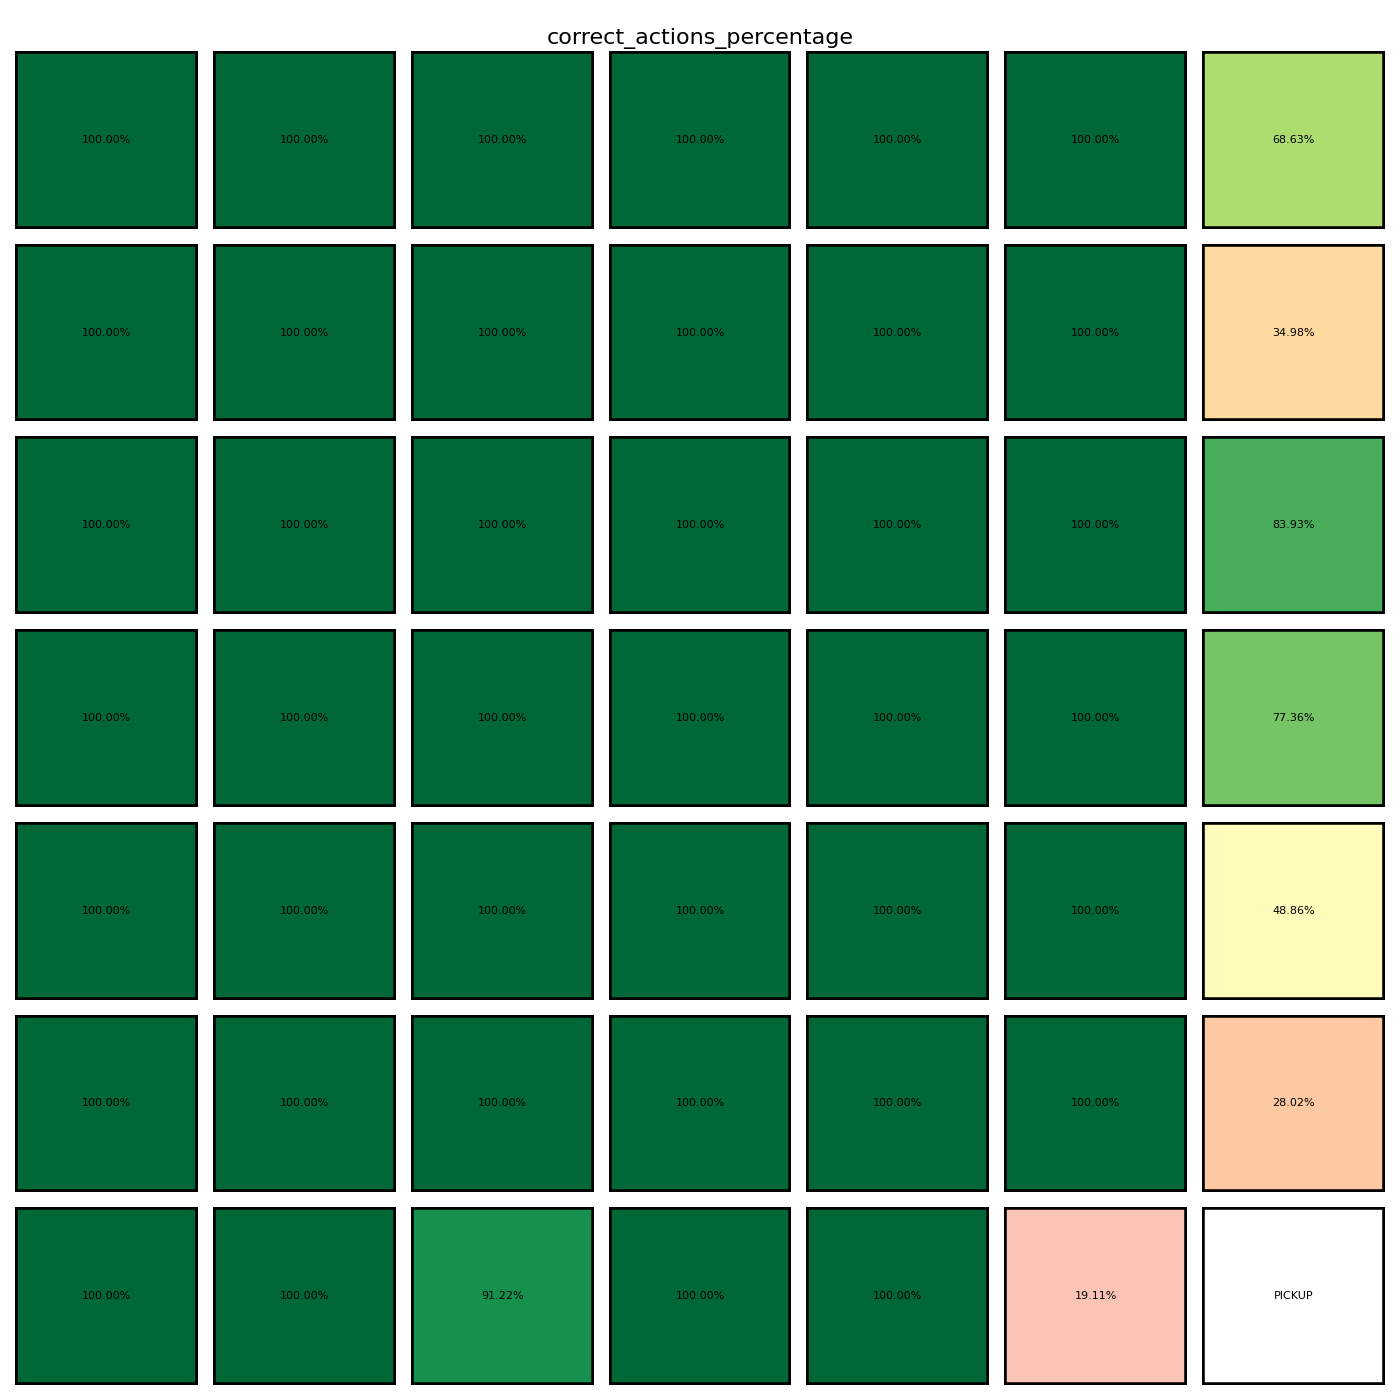
\includegraphics[width=\textwidth]{
      images/results_discussion/stateless/not_central/chm_pickup_bottom_right.png
    }
    \caption{Correctness Pickup Bottom Right}
    \label{fig:chm_pickup_bottom_right}
  \end{minipage}
  \hfill
  \begin{minipage}[b]{0.45\textwidth}
    \centering
    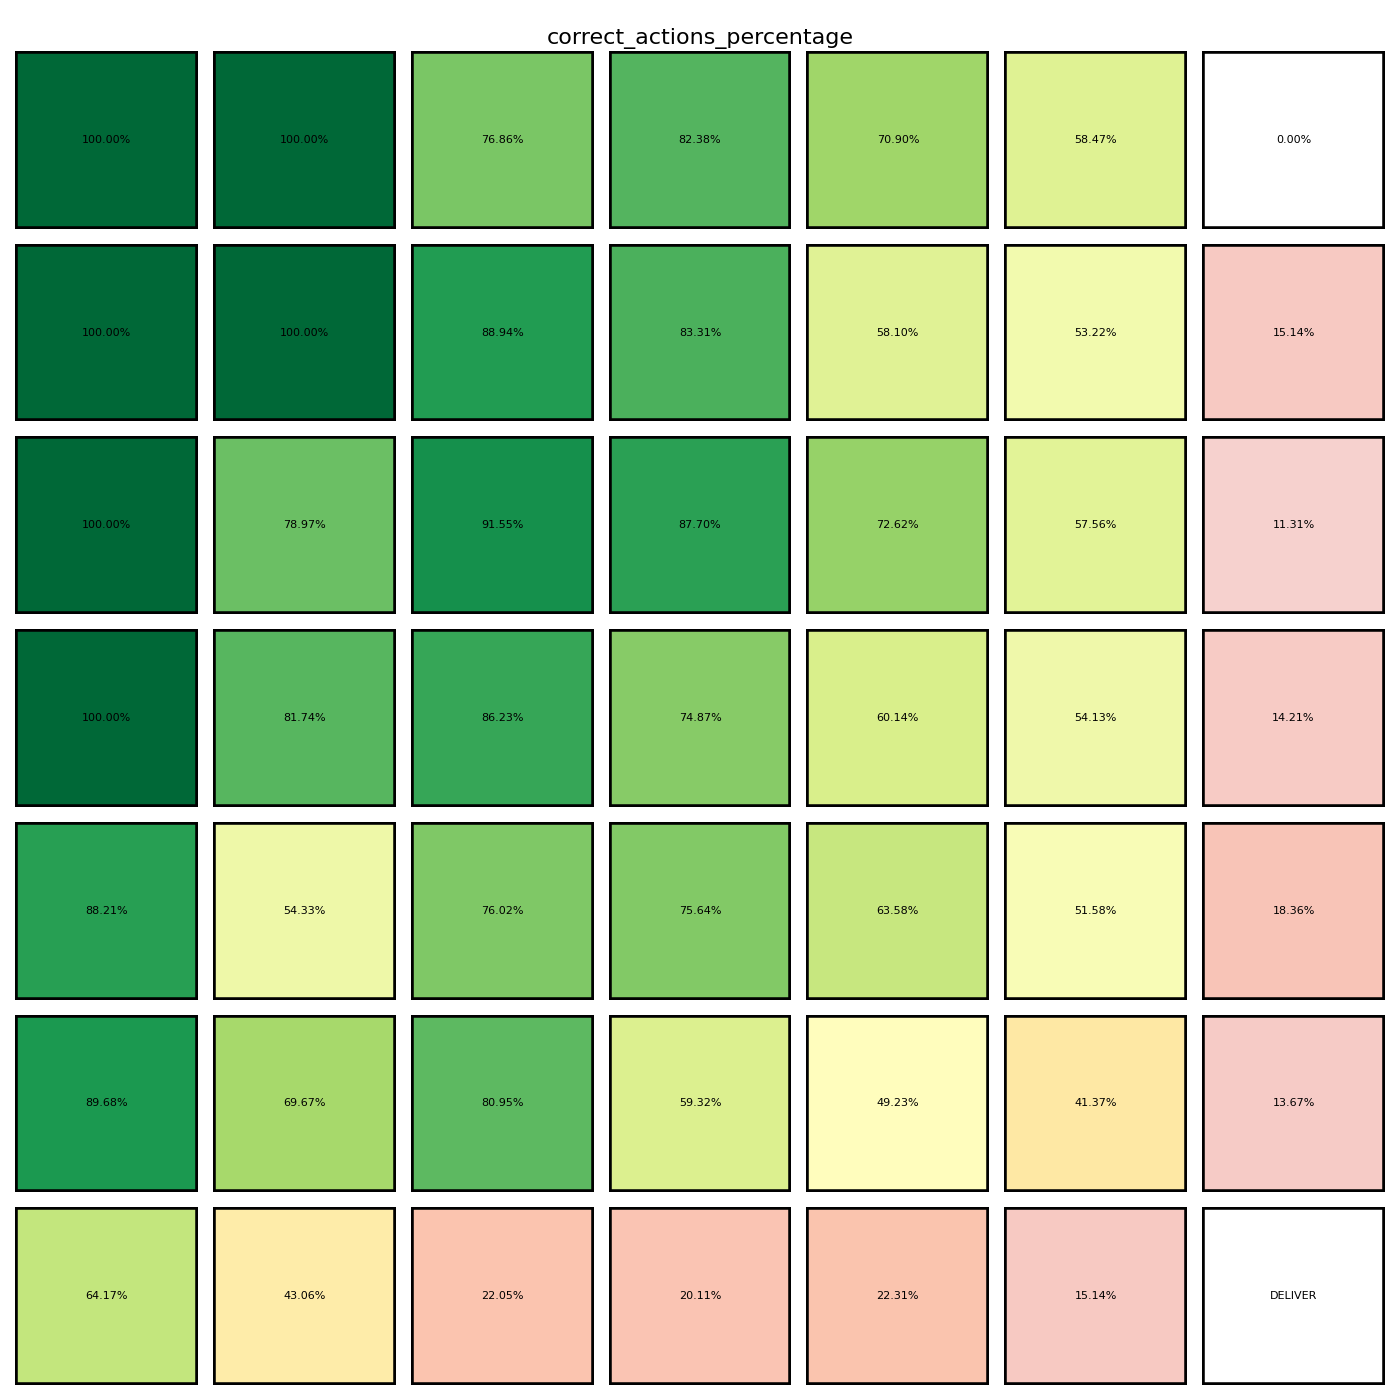
\includegraphics[width=\textwidth]{
      images/results_discussion/stateless/not_central/chm_deliver_bottom_right.png
    }
    \caption{Correctness Deliver Bottom Right}
    \label{fig:chm_deliver_bottom_right}
  \end{minipage}
  \caption{Correctness heatmaps for stateless agent with pickup and deliver
  goals in the bottom right corner of the map}
  \label{fig:stateless_bottom_right_correctness}
\end{figure}
\vspace{5mm}

These alternative goal placements provide valuable insights into the agent's
decision-making and can be seen as subsets of the larger map. For example, the
top-left portion of a 13x13 map with the goal in the center can be viewed as a
7x7 map with the goal in the bottom-right cell. At the same time, the bottom-left
portion of the 13x13 map with the center goal corresponds to a 7x7 map with the
top-right goal. This perspective brings us to the following topic, where a slice
with the same size from different maps is compared.

\vspace{5mm}
\begin{figure}[h]
  \centering
  \begin{minipage}[b]{0.19\textwidth}
    \centering
    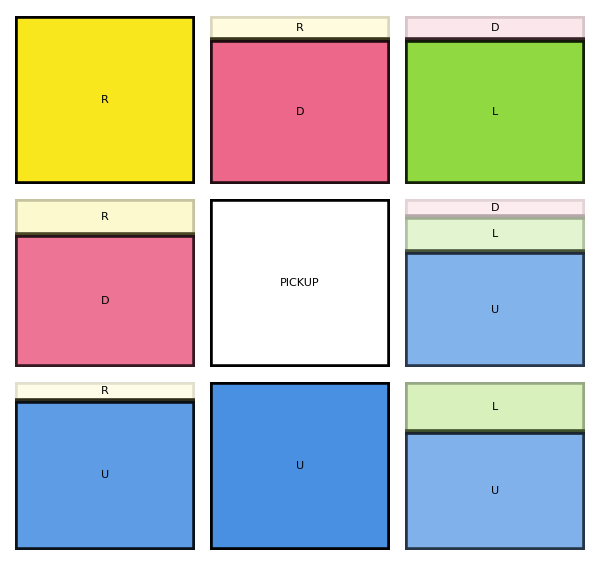
\includegraphics[width=\textwidth]{
      images/results_discussion/comparison/hm_3x3.png
    }
    \caption{3x3}
    \label{fig:hm_3x3}
  \end{minipage}
  \hfill
  \begin{minipage}[b]{0.19\textwidth}
    \centering
    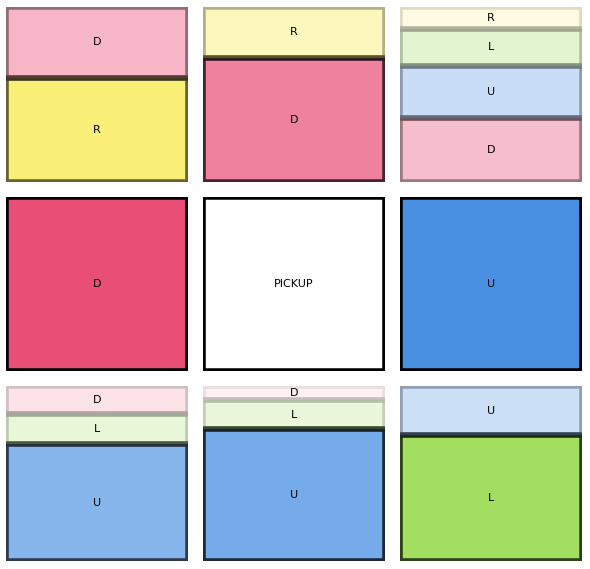
\includegraphics[width=\textwidth]{
      images/results_discussion/comparison/hm_5x5.png
    }
    \caption{5x5}
    \label{fig:hm_5x5}
  \end{minipage}
  \hfill
  \begin{minipage}[b]{0.19\textwidth}
    \centering
    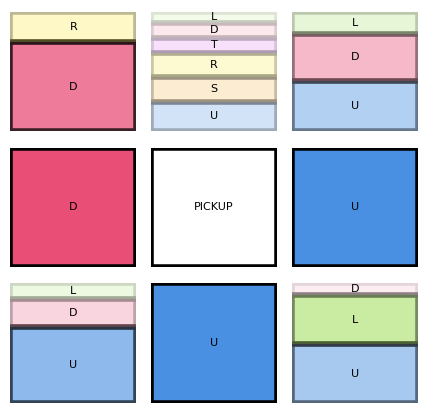
\includegraphics[width=\textwidth]{
      images/results_discussion/comparison/hm_7x7.png
    }
    \caption{7x7}
    \label{fig:hm_7x7}
  \end{minipage}
  \hfill
  \begin{minipage}[b]{0.19\textwidth}
    \centering
    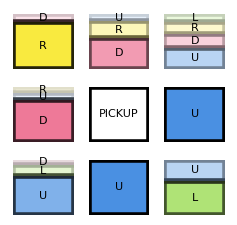
\includegraphics[width=\textwidth]{
      images/results_discussion/comparison/hm_13x13.png
    }
    \caption{13x13}
    \label{fig:hm_13x13}
  \end{minipage}
  \hfill
  \begin{minipage}[b]{0.19\textwidth}
    \centering
    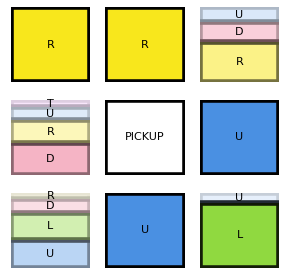
\includegraphics[width=\textwidth]{
      images/results_discussion/comparison/hm_21x21.png
    }
    \caption{21x21}
    \label{fig:hm_21x21}
  \end{minipage}
  \caption{Heatmaps for different map sizes}
  \label{fig:around_comparison}
\end{figure}
\vspace{5mm}

It is already visible in figure \ref{fig:stateless_deliver_heatmaps} but can be seen
better in figure \ref{fig:around_comparison}. Even if the values in the cells
around the goal are very similar, they are not the same. This may be due to the
fact that the LLM spreads the attention across all the prompt, and with a smaller
map, the map occupies less space in it.

\subsection{Goal position comparison}

A final analysis was conducted to determine whether the placement of the delivery
goal in different sections of the map affects the overall accuracy of the stateless
agent. Table \ref{tab:performance_21x21} presents performance metrics for the
21x21 grid in three configurations:
\begin{itemize}
  \item \textbf{Top Right (TR):} The delivery goal is positioned in the top-right
    corner;

  \item \textbf{Center (CN):} The delivery goal is placed in the center of the
    map;

  \item \textbf{Bottom Right (BR):} The delivery goal is located in the bottom-right
    corner.
\end{itemize}

\begin{table}[h]
  \centering
  \begin{tabular}{c|ccc|ccc}
              & top1 & top2 & top3 & top1\% & top2\% & top3\% \\
    \hline
    21x21\_TR & 378  & 429  & 433  & 0.859  & 0.975  & 0.984  \\
    21x21\_CN & 294  & 394  & 428  & 0.668  & 0.895  & 0.973  \\
    21x21\_BR & 371  & 416  & 417  & 0.843  & 0.945  & 0.948  \\
  \end{tabular}
  \caption{Performance metrics for different 21x21 configurations}
  \label{tab:performance_21x21}
\end{table}

From the data, we can draw several conclusions:
\begin{itemize}
  \item The top-right and bottom-right configurations exhibit similar performance,
    with top1 accuracy at 85.9\% and 84.3\%, respectively, as stated in Section
    \ref{sub:goal_positioning};

  \item The center goal configuration shows a notable drop in top1 accuracy to 66.8\%,
    confirming our earlier observation that finding a specific information hidden
    in the middle of a long text is more challenging;

  \item The difference between the top2 and top3 accuracy rates across the three
    configurations indicates that, even when the correct action is not the most
    probable choice, it is still frequently within the top-ranked options,
    meaning the model maintains a reasonable degree of decision-making
    reliability.
\end{itemize}

These results reinforce the hypothesis that stateless agents struggle most when
they must infer goal locations based on spatial relationships rather than
relying on explicit goal markers. Additionally, it confirms that the layout of
the prompt itself (how the map is structured in textual form) plays a role in
how effectively the LLM can interpret spatial cues.

\section{Stateful}
\label{sec:stateful}

Stateful means that we kept track of the chat history, so at every step, all the
past states and actions are available to the LLM. This allows the agent to build
an internal representation of the map and track its movements over time, enabling
more informed decision-making. The stateful approach integrates historical
context, which is especially beneficial for tasks where understanding the progression
of events is crucial; in this case it allows the agent to better understand the
map orientation.

One key advantage of a stateful agent is its ability to recover from errors. With
access to previous interactions, the LLM can identify patterns such as
repetitive loops or suboptimal paths. Recognizing these patterns, the agent is
able to adjust its strategy, replan its path, and ultimately increase the chance
of reaching the goal even after encountering execution errors or obstacles.

This translates to the fact that the agent is able to reach the goal even when
the stateless output does not find any correct action.

Moreover, accumulating past interactions enables the LLM to develop a more comprehensive
internal map of the environment. This cumulative knowledge is beneficial not
only for precise navigation but also when the environment may change or when
additional information is provided later in the interaction. The agent can correlate
new data with the stored context, providing a more robust response compared to a
stateless design, where each decision is made in isolation.

However, a stateful design does carry potential challenges. One significant issue
is the token limit imposed by the LLM. As the conversation history grows, managing
and condensing the context without losing essential details becomes critical.
Strategies such as summarizing less relevant parts of the dialogue or
periodically resetting portions of the context are often necessary to remain
within token constraints while still maintaining effective decision-making. They
have been tested in the form of sending the map in the first call, then wait and
send it again every 5 or 10 messages, but it either made the agent not performing
as desired or the sending of the map was still so frequent that the token limit was
reached fast.

\subsection{Path Visualization}
\begin{figure}[h]
  \centering
  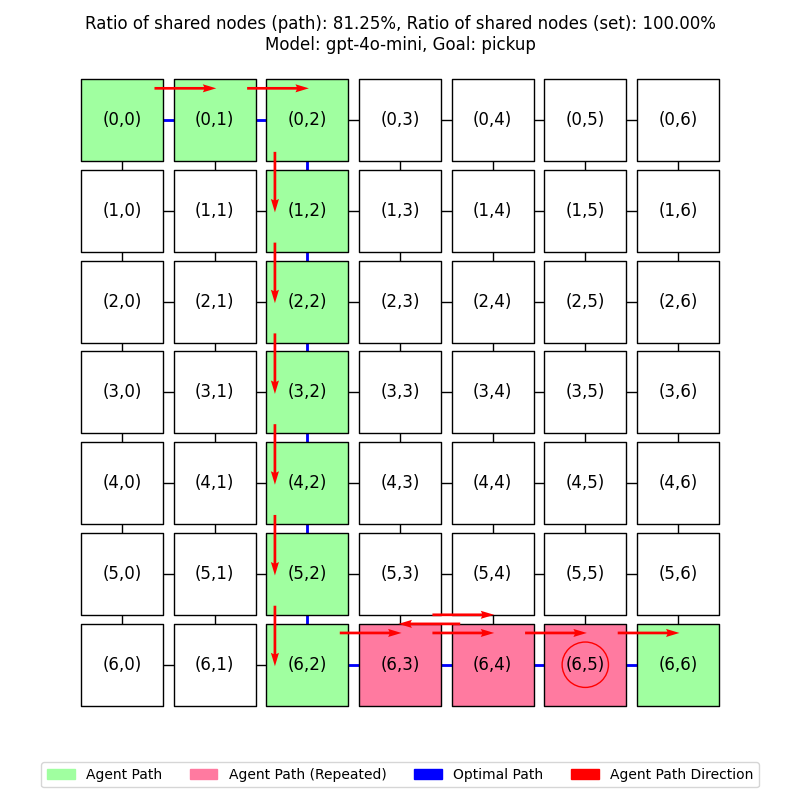
\includegraphics[width=0.5\textwidth]{
    images/results_discussion/stateful/pickupBR_7x7.png
  }
  \caption{Caption}
  \label{fig:stateful_path}
\end{figure}

A dedicated visualization script has been developed to illustrate the agent's
path on the map. This script identifies all optimal paths connecting the start and
the goal, selects the one sharing the highest number of common cells with the
agent's path, and then calculates both the percentage of overlapping cells and the
relative difference in path length. Figure \ref{fig:stateful_path} displays an
example output, highlighting that although the agent eventually reaches the goal,
it encounters difficulties navigating in the vicinity of the goal, as discussed in
Section \ref{sub:pickup_goal_at_the_center}.

\section{``Path Finding''}

Up to this point, we have observed that, in almost every instance, the KnowNo framework
consistently discarded actions related to the agent's goals, such as picking up
and delivering parcels. To determine whether these goal-related actions still contributed
significantly to the agent's uncertainty, we designed an experiment where the
objective was reduced to simply reaching a specific tile.

To implement this, we removed the pickup and delivery actions from the prompt while
keeping all other conditions unchanged. The goal was set up as just reaching a
specific tile, similarly to what the ``Pickup goal'' requires. By doing so, we aimed
to isolate and examine the role of these actions in influencing the agent's uncertainty.
The results of this experiment are presented in Figure \ref{fig:path_finding}. This
approach aligns with our systematic methodology, as previously discussed in
Section \ref{sec:closest_cell_to_the_goal}, where we progressively simplified the
agent's goals to identify potential limitations in decision-making.

A meaningful comparison can be drawn between these results and those obtained from
a scenario in which the agent operated on a 5x5 grid with a pickup goal located at
the center. Since both setups shared the same prompt structure, this comparison allows
us to assess whether the presence of goal-related actions had a significant impact
on the agent's uncertainty. The results from the 5x5 pickup scenario, previously
discussed, can be found in Figure \ref{fig:hm_5x5_pickup} and Figure
\ref{fig:chm_5x5_pickup}.

\begin{figure}[h!]
  \centering
  \begin{minipage}[b]{0.45\textwidth}
    \centering
    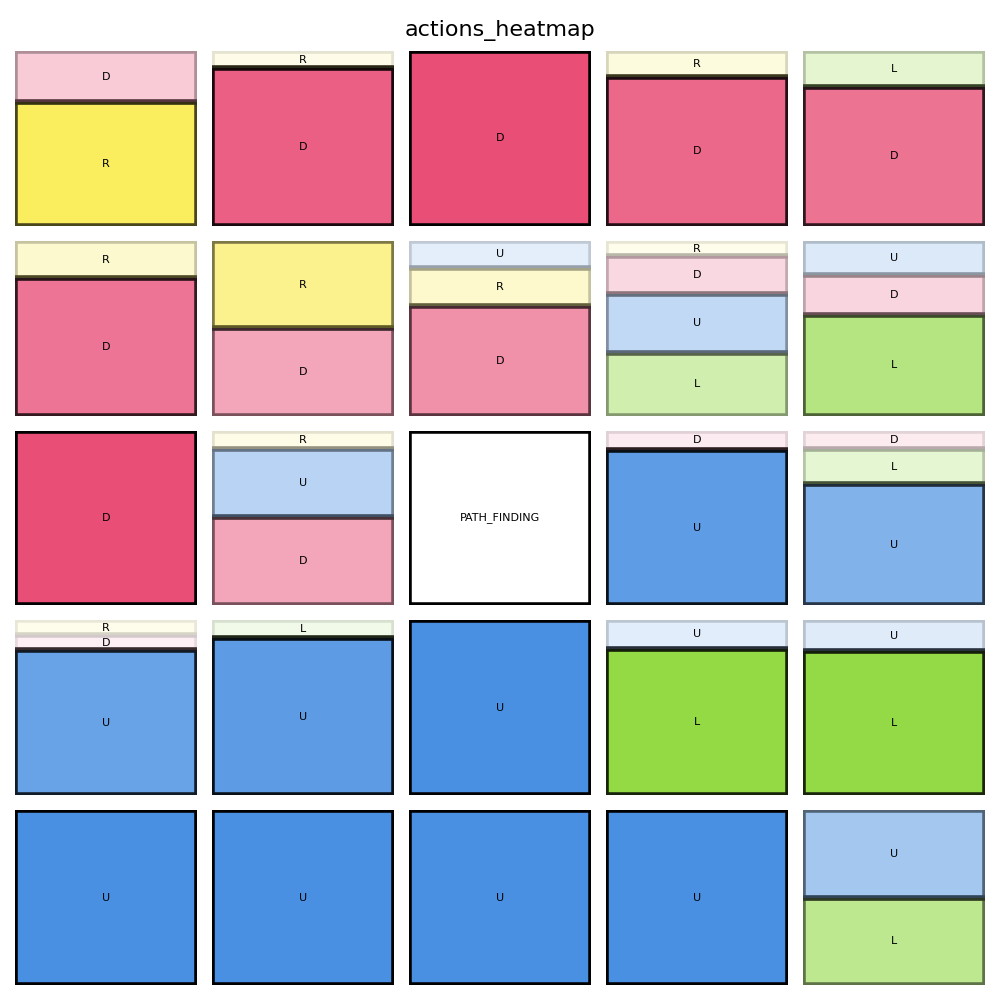
\includegraphics[width=\textwidth]{
      images/results_discussion/path_finding/actions_heatmap.png
    }
    \caption{Correctness pathfinding }
    \label{fig:path_finding_hm}
  \end{minipage}
  \hfill
  \begin{minipage}[b]{0.45\textwidth}
    \centering
    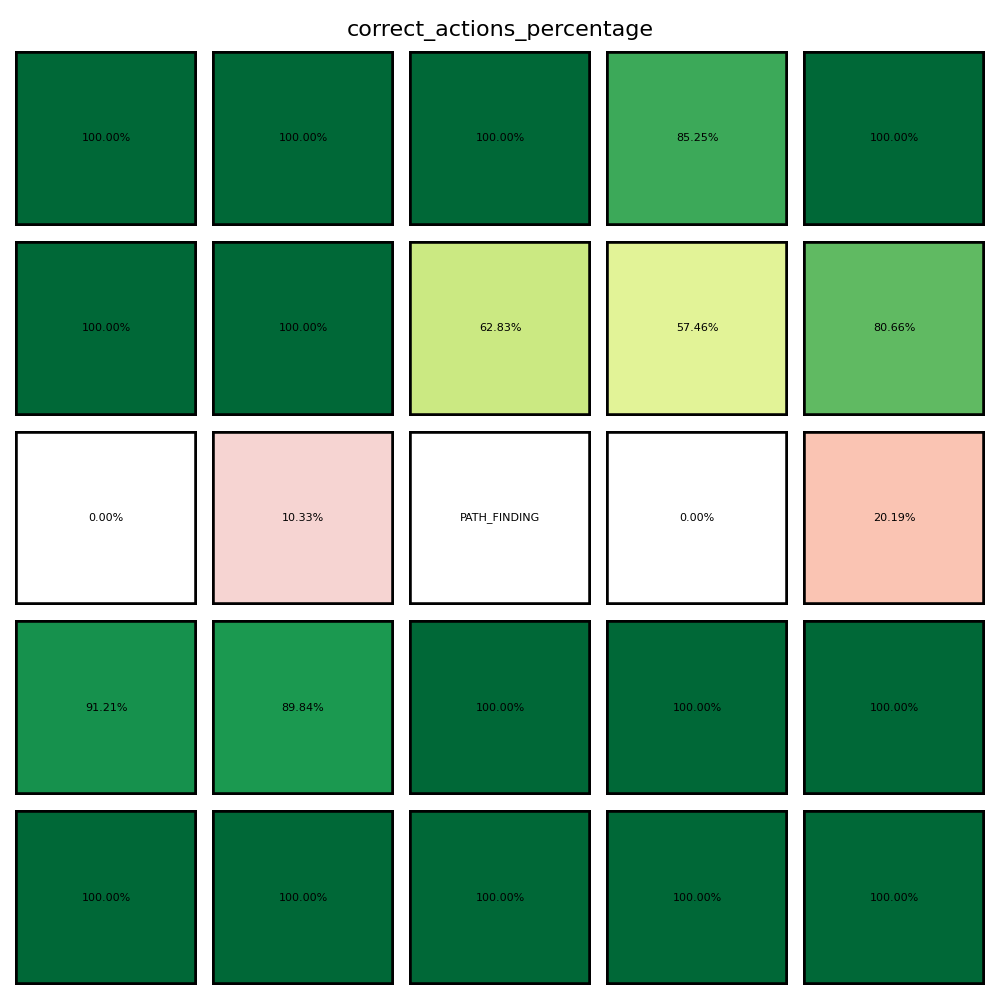
\includegraphics[width=\textwidth]{
      images/results_discussion/path_finding/correct_actions_percentage_PERC.png
    }
    \caption{Correctness Deliver Top Right}
    \label{fig:path_finding_corr}
  \end{minipage}
  \caption{Correctness heatmaps for stateless agent with pickup and deliver
  goals in the top right corner of the map}
  \label{fig:path_finding}
\end{figure}

The outcomes of both experiments are remarkably similar, revealing identical
areas of high and low uncertainty. This suggests that goal-related actions are not
the primary source of uncertainty in the agent's decision-making process.
Furthermore, it reinforces the idea that the structure of the prompt, carefully
designed based on the literature reviewed as explained in Section
\ref{sec:prompt_creation_choices}, is not a key factor contributing to uncertainty.
Instead, the observed uncertainty may be more closely linked to the inherent limitations
of the LLM itself.

\section{Stateless \& Stateful - Performance Summary}
\label{sec:stateless_and_stateful_combined_results}

Experimental results in this study indicate that the stateful configuration
outperforms the stateless one in terms of accuracy and goal attainment, particularly
in larger maps. The ability to trace its previous actions and incorporate
historical context leads to a more adaptive and flexible approach, which is evident
in tasks requiring dynamic path corrections and strategic foresight. During the
first stages of the experiments, where we tried the limits of the token input size,
the stateless agent was not able at all to achieve any goal in maps bigger than
21x21, while the stateful agent was on the correct path but blocked by the token
limit. This is a clear demonstration of the stateful agent's superior
performance in handling complex spatial navigation tasks.

Additionally, the stateful method aligns well with the inherent strengths of large
language models as few-shot learners \cite{brown2020languagemodelsfewshotlearners}.
The continuous integration of historical data and real-time inputs allows the
agent to refine its internal representation of the map, which significantly improves
its overall navigational performance. This dynamic adjustment provides
resilience against uncertainties common in spatial navigation tasks.

Practically speaking, the stateful agent demonstrates a clear advantage in navigating
the "problematic" areas of the maps, particularly in the top-right quadrant, where
the stateless version exhibits significant uncertainty. This improvement arises
from the stateful agent's ability to retain memory of its past actions, enabling
it to recognize and correct mistakes. If it takes a step in the wrong direction,
it can backtrack to a previous cell and attempt an alternative route, ultimately
increasing its chances of reaching the goal efficiently.

However, as the map size increases, both versions encounter growing difficulties,
with the top-right quadrant consistently presenting the most challenges. This
issue stems from the nature of decision-making in that region: many cells offer multiple
actions with nearly equal probabilities, making it harder for the agent to
determine the optimal path. While the relative frequency of these problematic cells
remains constant as the map scales up, the absolute number of such cells
increases substantially. For example, in a small 3x3 map, a single problematic cell
is manageable, as the agent can quickly backtrack and reach the goal. In contrast,
in a much larger 21x21 map, there could be as many as 49 problematic cells. Even
though this proportion is the same in percentage terms, the larger map exacerbates
the challenge. With more problematic cells spread across a wider area, the agent
is more likely to make a series of unfortunate steps, potentially getting
trapped in a suboptimal loop and failing to recover efficiently. This issue is particularly
severe for the stateless agent, but even the stateful agent, despite its ability
to backtrack, can struggle to escape if the problematic region is too large.

A summary of their performance are presented in the table \ref{tab:svss}, where the
agent was tasked to pickup a parcel in the bottom left cell and started in the top
right cell (since it is the most problematic area). The recorded action count
includes the pickup action.

\vspace{5mm}
\begin{table}[h]
  \centering
  \begin{tabular}{c|cc|c}
    \textbf{Map Size} & \textbf{Stateless} & \textbf{Stateful} & \textbf{Mathematical Best} \\
    \hline
    13x13             & 41                 & 39 actions        & 25 actions                 \\
    7x7               & 27                 & 21 actions        & 13 actions                 \\
    5x5               & 14 actions         & 11 actions        & 9 actions                  \\
    3x3               & 11 actions         & 9 actions         & 5 actions                  \\
  \end{tabular}
  \caption{Number of actions in different map sizes using GPT-4o-mini}
  \label{tab:svss}
\end{table}
\vspace{5mm}

In summary, although the stateful approach can introduce computational overhead
due to increased context size, its advantages in enhancing navigational accuracy,
recovery from errors, and adaptive decision-making render it a vital component in
modern agent design. Still, the limitation of the token limit is a significant drawback
that may be overcome by more powerful models, that may introduce better results
out of the box as well as a longer context window.

\section{Insights from the Closest Cell to the Goal Approach}
\label{sec:closest_cell_to_the_goal_results}

As detailed in Section \ref{sec:closest_cell_to_the_goal}, this approach aimed
to simplify the agent's decision-making process by breaking it down into two
sequential steps: (1) identifying the best adjacent cell to move toward and (2) selecting
the correct action to reach that cell. The motivation behind this decomposition
was to reduce the complexity of the global path-finding task and test whether
the agent could make more reliable local decisions.

Although this method was not central to our primary experiments, we include it here
for completeness, as analyzing its shortcomings provided useful insights into
the agent's limitations.

However, despite its structured nature, this method introduced new challenges
rather than resolving the agent's decision-making issues. In particular, two key
limitations emerged:
\begin{itemize}
  \item Ambiguity in selecting the ``best" cell: In many cases, more than one
    neighboring cell reduced the distance to the goal, making it unclear which one
    the agent should prioritize and more difficult to us to record structured data
    to analyze. As illustrated in Figure \ref{fig:extra2}, the decision was not always
    straightforward, and slight variations in prompt phrasing could lead the LLM
    to prefer different paths, even when multiple valid choices existed;

  \item Compounding errors in high-uncertainty areas: This two-step approach
    inadvertently introduced an additional layer of failure. If the agent misidentified
    the best neighboring cell, it would inherently lead to a suboptimal move, even
    if the second step—choosing the action—was executed perfectly. This doubled
    the impact of errors, particularly in ambiguous or low-information regions of
    the map, where uncertainty was already high.
\end{itemize}

\vspace{7mm}
\begin{figure}[h!]
  \centering
  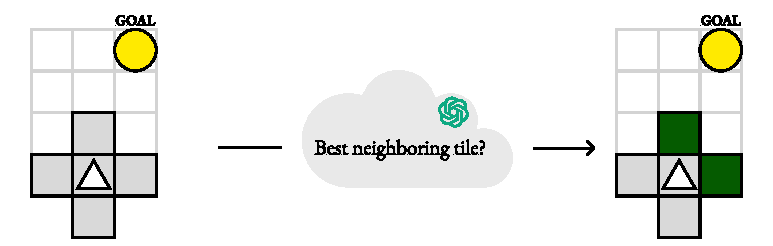
\includegraphics[width=.66\textwidth]{images/results_discussion/extra2.pdf}
  \caption{Two-steps decision making example}
  \label{fig:extra2}
\end{figure}
\vspace{7mm}

  % Conclusions
  \chapter{Future Works}
\label{cha:future_works}
  \chapter{Conclusions}
\label{cha:conclusions}

\lipsum[1]
  \endgroup

  % Bibliography
  \addcontentsline{toc}{chapter}{Bibliography}
  % Alphabetical order of authors
  \bibliographystyle{plain}
  \bibliography{bibliography.bib}

  % Attachments
  \titleformat{\chapter} {\normalfont\Huge\bfseries}{Appendix \thechapter}{1em}{}
  \appendix
  \chapter{Attachment - Prompts}
\label{cha:attachment}
\begin{codewindow}
  [Prompt] \lstset{style=promptstyle, language=prompt, caption={Example of a prompt used in the second agent implementation, see Section \ref{sec:second_approach}},
  label={lst:apx:second_agent_prompt}} \begin{lstlisting}
You are a delivery agent in a web-based game I am going to give you the raw information I receive from the server and the possible actions. You have to take (pickup) the parcel and ship (deliver) it in a delivery tile.
Don't loop using the same moves.
If the information does not change, it means you are choosing the wrong actions.
Raw 'onMap' response: {"width":2,"height":5,"tiles":[{"x":0,"y":0,"delivery":false},{"x":0,"y":1,"delivery":true},{"x":1,"y":0,"delivery":false},{"x":1,"y":1,"delivery":false},{"x":2,"y":0,"delivery":false},{"x":2,"y":1,"delivery":false},{"x":3,"y":0,"delivery":false},{"x":3,"y":1,"delivery":false},{"x":4,"y":0,"delivery":false},{"x":4,"y":1,"delivery":false}]}

Raw 'onYou' response: {"id":"75d4e78ed8e","name":"raw_llm_agent","x":3,"y":1,"score":0}

Raw 'onParcelsSensing' response: [{"id":"p0","x":3,"y":0,"carriedBy":null,"reward":10}]

ACTIONS you can do:
U): move up
D): move down
L): move left
R): move right
T): take the parcel that is in your tile
S): ship a parcel (you must be in a delivery=true tile)
Don't explain the reasoning and don't add any comment, just provide the action.
What is your next action?
\end{lstlisting}
\end{codewindow}
\clearpage
\begin{codewindow}
  [Prompt] \lstset{style=promptstyle, language=prompt, caption={Example of a prompt used in the first agent implementation, see Section \ref{sec:first_approach}},
  label={lst:apx:first_agent_prompt}} \begin{lstlisting}
You are a delivery agent in a web-based game and I want to test your ability. You are in a grid world (represented with a matrix) with some obstacles and some parcels to deliver.
Parcels are generated at random on random free spots.
The value of the parcels lowers as the time passes, so you should deliver them as soon as possible.
Your view of the world is limited to a certain distance, so you can only see the parcels and the delivery points that are close to you.
MAP:
1 1 1 1 1
1 1 P 1 1
1 1 1 1 1
2 A 1 1 1
1 1 1 1 1

LEGEND:
- A: you (the Agent) are in this position;
- 1: you can move in this position;
- 2: you can deliver a parcel in this position (and also move there);
- P: a parcel is in this position;
- X: you are in the same position of a parcel;
- Q: you are in the delivery/shipping point;

ACTIONS you can do:
- U: move up
- D: move down
- L: move left
- R: move right
- T: take a parcel
- S: ship a parcel

You have 1 parcels to deliver.
Important rules:
- If you have 0 parcels, you must look for the closest parcel to pick up.
- If you are going to deliver >0 parcels and on the way you find 1 parcel, you should go and pick it up before shipping.
- If you have at least 1 parcel, your goal should be to deliver it/them to the closest delivery point. The more parcels you have, the more important it is to deliver them as soon as possible.
- If you can't see any delivery point, just move around to explore the map until one enters your field of view, then go and deliver the parcels.
- If there is no parcel in the map, just move around to explore the map until one parcel spawns, then go and get it.

You want to maximize your score by delivering the most possible number of parcels. You can pickup multiple parcels and deliver them in the same delivery point.
Don't explain the reasoning and don't add any comment, just provide the action.
Try to not go back and forth, it's a waste of time, so use the conversation history to your advantage.
Example: if you want to go down, just answer 'D'.
The closest delivery point is right and up from you.
What is your next action?
\end{lstlisting}
\end{codewindow}
\end{document}